%Bayesian_tools.tex
%
\documentclass[latex]{beamer}
\usepackage{graphicx,xspace,color}
\usepackage[utf8]{inputenc}
\usepackage[T1]{fontenc}
\usepackage[francais]{babel}
\usepackage{subfig}
\usepackage[french,linesnumbered,algoruled]{algorithm2e}
\usepackage{algorithmic}
\usepackage{multirow}
\usepackage{pstricks}
\usepackage{pst-grad} % For gradients
\usepackage{pst-plot} % For axes
\usepackage{epsfig}
\usepackage[babel=true]{csquotes}
\usepackage{float}
\usepackage{multirow}
\usepackage{epstopdf}
\epstopdfsetup{suffix=}
\setbeamertemplate{bibliography item}[text]
\setbeamercolor*{bibliography entry author}{fg=black}
\setbeamercolor*{bibliography item}{fg=black}

\graphicspath{{figuresFully3D2017/}}
\mode<presentation>
{
  \usetheme{default}
  \setbeamercovered{transparent}
}
%------------------MACROS -----------------------
%\def\inputdir{/home/djafari/2015/Inputs/}
% Document LaTeX based on Alphabet by Guy Lebesnerai
% Ali Mohammad-Djafari (janvier 2013)
% Objectif : Definitions for bold Math writing
%
% b pour bold italique : 		\ab \Ab
% v pour bold droit :    		\av \Av
% D pour droit :         		\aD \AD
% c pour cursif :					\Ac
% cb pour cursif bold:       		\Acb
% Grec italique: 				\alphab \Sigmab

% h pour \widehat:         		\ah \Ah \alphah \Sigmah
% t pour \widetilde:       		\at \At \alphat \Sigmat
% bt pour \widetilde\bold: 		\abt \Abt \alphabt \Sigmabt
% bh pour \widehat\bold:   		\abh \Abh \alphabh \Sigmabh

\typeout{\space}
\typeout{\space\space\space\space Fichier 'alphabet.tex' -- LSS 1994/95/99}
\typeout{\space\space\space\space (necessite les packages xspace, amsmath, bbm)}
\typeout{\space}

%\RequirePackage{amsmath}
%\RequirePackage{xspace}
%\RequirePackage{oldgerm}		% 04.06.2003   Pour les alphabet Gauthiques

%-------------------------------------------
% DEFINITIONS PRELIMINAIRES 

\def\XS{\xspace}
\DeclareMathAlphabet{\mathb}{OML}{cmm}{b}{it}
\def\sbm#1{\ensuremath{\mathb{#1}}}                % Style gras italique (necessite amsmath)           
\def\sbmm#1{\ensuremath{\boldsymbol{#1}}}          % Style gras italique (necessite amsmath)           
\def\sdm#1{\ensuremath{\mathrm{#1}}}               % Style droit en math
\def\sbv#1{\ensuremath{\mathbf{#1}}}               % Style gras droit
\def\scu#1{\ensuremath{\mathcal{#1\XS}}}           % Style cursif
\def\scb#1{\ensuremath{\boldsymbol{\mathcal{#1}}}} % Style gras cursif
\def\sbl#1{\ensuremath{\mathbbm{#1}}}              % Style blackboard (necessite bbm)
\def\bm#1{\mbox{\boldmath $#1$}}
%-------------------------------------------

% ALPHABET GRAS ITALIQUE, taille adaptative
\def\Ab{{\sbm{A}}\XS}  \def\ab{{\sbm{a}}\XS}
\def\Bb{{\sbm{B}}\XS}  \def\bb{{\sbm{b}}\XS}
\def\Cb{{\sbm{C}}\XS}  \def\cb{{\sbm{c}}\XS}
\def\Db{{\sbm{D}}\XS}  \def\db{{\sbm{d}}\XS}
\def\Eb{{\sbm{E}}\XS}  \def\eb{{\sbm{e}}\XS}
\def\Fb{{\sbm{F}}\XS}  \def\fb{{\sbm{f}}\XS}
\def\Gb{{\sbm{G}}\XS}  \def\gb{{\sbm{g}}\XS}
\def\Hb{{\sbm{H}}\XS}  \def\hb{{\sbm{h}}\XS}
\def\Ib{{\sbm{I}}\XS}  \def\ib{{\sbm{i}}\XS}
\def\Jb{{\sbm{J}}\XS}  \def\jb{{\sbm{j}}\XS}
\def\Kb{{\sbm{K}}\XS}  \def\kb{{\sbm{k}}\XS}
\def\Lb{{\sbm{L}}\XS}  \def\lb{{\sbm{l}}\XS}
\def\Mb{{\sbm{M}}\XS}  \def\mb{{\sbm{m}}\XS}
\def\Nb{{\sbm{N}}\XS}  \def\nb{{\sbm{n}}\XS}
\def\Ob{{\sbm{O}}\XS}  \def\ob{{\sbm{o}}\XS}
\def\Pb{{\sbm{P}}\XS}  \def\pb{{\sbm{p}}\XS}
\def\Qb{{\sbm{Q}}\XS}  \def\qb{{\sbm{q}}\XS}
\def\Rb{{\sbm{R}}\XS}  \def\rb{{\sbm{r}}\XS}
\def\Sb{{\sbm{S}}\XS}  \def\sb{{\sbm{s}}\XS}
\def\Tb{{\sbm{T}}\XS}  \def\tb{{\sbm{t}}\XS}
\def\Ub{{\sbm{U}}\XS}  \def\ub{{\sbm{u}}\XS}
\def\Vb{{\sbm{V}}\XS}  \def\vb{{\sbm{v}}\XS}
\def\Wb{{\sbm{W}}\XS}  \def\wb{{\sbm{w}}\XS}
\def\Xb{{\sbm{X}}\XS}  \def\xb{{\sbm{x}}\XS}
\def\Yb{{\sbm{Y}}\XS}  \def\yb{{\sbm{y}}\XS}
\def\Zb{{\sbm{Z}}\XS}  \def\zb{{\sbm{z}}\XS}

% ALPHABET CURSIF MAJUSCULE, taille adaptative
% Cursif,               % Cursif gras
\def\Ac{{\scu{A}}\XS}   \def\Acb{{\scb{A}}\XS}
\def\Bc{{\scu{B}}\XS}   \def\Bcb{{\scb{B}}\XS}
\def\Cc{{\scu{C}}\XS}   \def\Ccb{{\scb{C}}\XS}
\def\Dc{{\scu{D}}\XS}   \def\Dcb{{\scb{D}}\XS}
\def\Ec{{\scu{E}}\XS}   \def\Ecb{{\scb{E}}\XS}
\def\Fc{{\scu{F}}\XS}   \def\Fcb{{\scb{F}}\XS}
\def\Gc{{\scu{G}}\XS}   \def\Gcb{{\scb{G}}\XS}
\def\Hc{{\scu{H}}\XS}   \def\Hcb{{\scb{H}}\XS}
\def\Ic{{\scu{I}}\XS}   \def\Icb{{\scb{I}}\XS}
\def\Jc{{\scu{J}}\XS}   \def\Jcb{{\scb{J}}\XS}
\def\Kc{{\scu{K}}\XS}   \def\Kcb{{\scb{K}}\XS}
\def\Lc{{\scu{L}}\XS}   \def\Lcb{{\scb{L}}\XS}
\def\Mc{{\scu{M}}\XS}   \def\Mcb{{\scb{M}}\XS}
\def\Nc{{\scu{N}}\XS}   \def\Ncb{{\scb{N}}\XS}
\def\Oc{{\scu{O}}\XS}   \def\Ocb{{\scb{O}}\XS}
\def\Pc{{\scu{P}}\XS}   \def\Pcb{{\scb{P}}\XS}
\def\Qc{{\scu{Q}}\XS}   \def\Qcb{{\scb{Q}}\XS}
\def\Rc{{\scu{R}}\XS}   \def\Rcb{{\scb{R}}\XS}
\def\Sc{{\scu{S}}\XS}   \def\Scb{{\scb{S}}\XS}
\def\Tc{{\scu{T}}\XS}   \def\Tcb{{\scb{T}}\XS}
\def\Uc{{\scu{U}}\XS}   \def\Ucb{{\scb{U}}\XS}
\def\Vc{{\scu{V}}\XS}   \def\Vcb{{\scb{V}}\XS}
\def\Wc{{\scu{W}}\XS}   \def\Wcb{{\scb{W}}\XS}
\def\Xc{{\scu{X}}\XS}   \def\Xcb{{\scb{X}}\XS}
\def\Yc{{\scu{Y}}\XS}   \def\Ycb{{\scb{Y}}\XS}
\def\Zc{{\scu{Z}}\XS}   \def\Zcb{{\scb{Z}}\XS}

% ALPHABET DROIT EN MATHS, taille adaptative
\def\AD{{\sdm{A}}\XS}  \def\aD{{\sdm{a}}\XS}
\def\BD{{\sdm{B}}\XS}  \def\bD{{\sdm{b}}\XS}
\def\CD{{\sdm{C}}\XS}  \def\cD{{\sdm{c}}\XS}
\def\DD{{\sdm{D}}\XS}  \def\dD{{\sdm{d}}\XS}
\def\ED{{\sdm{E}}\XS}  \def\eD{{\sdm{e}}\XS}
\def\FD{{\sdm{F}}\XS}  \def\fD{{\sdm{f}}\XS}
\def\GD{{\sdm{G}}\XS}  \def\gD{{\sdm{g}}\XS}
\def\HD{{\sdm{H}}\XS}  \def\hD{{\sdm{h}}\XS}
\def\ID{{\sdm{I}}\XS}  \def\iD{{\sdm{i}}\XS}
\def\JD{{\sdm{J}}\XS}  \def\jD{{\sdm{j}}\XS}
\def\KD{{\sdm{K}}\XS}  \def\kD{{\sdm{k}}\XS}
\def\LD{{\sdm{L}}\XS}  \def\lD{{\sdm{l}}\XS}
\def\MD{{\sdm{M}}\XS}  \def\mD{{\sdm{m}}\XS}
\def\ND{{\sdm{N}}\XS}  \def\nD{{\sdm{n}}\XS}
\def\OD{{\sdm{O}}\XS}  \def\oD{{\sdm{o}}\XS}
\def\PD{{\sdm{P}}\XS}  \def\pD{{\sdm{p}}\XS}
\def\QD{{\sdm{Q}}\XS}  \def\qD{{\sdm{q}}\XS}
\def\RD{{\sdm{R}}\XS}  \def\rD{{\sdm{r}}\XS}
\def\SD{{\sdm{S}}\XS}  \def\sD{{\sdm{s}}\XS}
\def\TD{{\sdm{T}}\XS}  \def\tD{{\sdm{t}}\XS}
\def\UD{{\sdm{U}}\XS}  \def\uD{{\sdm{u}}\XS}
\def\VD{{\sdm{V}}\XS}  \def\vD{{\sdm{D}}\XS}
\def\WD{{\sdm{W}}\XS}  \def\wD{{\sdm{w}}\XS}
\def\XD{{\sdm{X}}\XS}  \def\xD{{\sdm{x}}\XS}
\def\YD{{\sdm{Y}}\XS}  \def\yD{{\sdm{y}}\XS}
\def\ZD{{\sdm{Z}}\XS}  \def\zD{{\sdm{z}}\XS}

% ALPHABET GRAS DROIT, taille adaptative
\def\Av{{\sbv{A}}\XS}  \def\av{{\sbv{a}}\XS}
\def\Bv{{\sbv{B}}\XS}  \def\bv{{\sbv{b}}\XS}
\def\Cv{{\sbv{C}}\XS}  \def\cv{{\sbv{c}}\XS}
\def\Dv{{\sbv{D}}\XS}  \def\dv{{\sbv{d}}\XS}
\def\Ev{{\sbv{E}}\XS}  \def\ev{{\sbv{e}}\XS}
\def\Fv{{\sbv{F}}\XS}  \def\fv{{\sbv{f}}\XS}
\def\Gv{{\sbv{G}}\XS}  \def\gv{{\sbv{g}}\XS}
\def\Hv{{\sbv{H}}\XS}  \def\hv{{\sbv{h}}\XS}
\def\Iv{{\sbv{I}}\XS}  \def\iv{{\sbv{i}}\XS}
\def\Jv{{\sbv{J}}\XS}  \def\jv{{\sbv{j}}\XS}
\def\Kv{{\sbv{K}}\XS}  \def\kv{{\sbv{k}}\XS}
\def\Lv{{\sbv{L}}\XS}  \def\lv{{\sbv{l}}\XS}
\def\Mv{{\sbv{M}}\XS}  \def\mv{{\sbv{m}}\XS}
\def\Nv{{\sbv{N}}\XS}  \def\nv{{\sbv{n}}\XS}
\def\Ov{{\sbv{O}}\XS}  \def\ov{{\sbv{o}}\XS}
\def\Pv{{\sbv{P}}\XS}  \def\pv{{\sbv{p}}\XS}
\def\Qv{{\sbv{Q}}\XS}  \def\qv{{\sbv{q}}\XS}
\def\Rv{{\sbv{R}}\XS}  \def\rv{{\sbv{r}}\XS}
\def\Sv{{\sbv{S}}\XS}  \def\sv{{\sbv{s}}\XS}
\def\Tv{{\sbv{T}}\XS}  \def\tv{{\sbv{t}}\XS}
\def\Uv{{\sbv{U}}\XS}  \def\uv{{\sbv{u}}\XS}
\def\Vv{{\sbv{V}}\XS}  \def\vv{{\sbv{v}}\XS}
\def\Wv{{\sbv{W}}\XS}  \def\wv{{\sbv{w}}\XS}
\def\Xv{{\sbv{X}}\XS}  \def\xv{{\sbv{x}}\XS}
\def\Yv{{\sbv{Y}}\XS}  \def\yv{{\sbv{y}}\XS}
\def\Zv{{\sbv{Z}}\XS}  \def\zv{{\sbv{z}}\XS}

% ALPHABET GREC GRAS italique, taille adaptative
\def\alphab{{\sbmm{\alpha}}\XS}
\def\betab{{\sbmm{\beta}}\XS}
\def\gammab{{\sbmm{\gamma}}\XS}      \def\Gammab{{\sbmm{\Gamma}}\XS}
\def\deltab{{\sbmm{\delta}}\XS}      \def\Deltab{{\sbmm{\Delta}}\XS}
\def\epsilonb{{\sbmm{\epsilon}}\XS}
\def\varepsilonb{{\sbmm{\varepsilon}}\XS}
\def\etab{{\sbmm{\eta}}\XS}
\def\thetab{{\sbmm{\theta}}\XS}      \def\Thetab{{\sbmm{\Theta}}\XS}
\def\varthetab{{\sbmm{\vartheta}}\XS}
\def\iotab{{\sbmm{\iota}}\XS}
\def\kappab{{\sbmm{\kappa}}\XS}
\def\varkappab{{\sbmm{\varkappa}}\XS}
\def\lambdab{{\sbmm{\lambda}}\XS}     \def\Lambdab{{\sbmm{\Lambda}}\XS}
\def\mub{{\sbmm{\mu}}\XS}
\def\nub{{\sbmm{\nu}}\XS}
\def\xib{{\sbmm{\xi}}\XS}         		\def\Xib{{\sbmm{\Xi}}\XS}
\def\pib{{\sbmm{\pi}}\XS}         		\def\Pib{{\sbmm{\Pi}}\XS}
\def\varpib{{\sbmm{\varpi}}\XS}
\def\rhob{{\sbmm{\rho}}\XS}
\def\varrhob{{\sbmm{\varrho}}\XS}
\def\sigmab{{\sbmm{\sigma}}\XS}      	\def\Sigmab{{\sbmm{\Sigma}}\XS}
\def\varsigmab{{\sbmm{\varsigma}}\XS}   \def\Varsigmab{{\sbmm{\Varsigma}}\XS}
\def\phib{{\sbmm{\phi}}\XS}        		\def\Phib{{\sbmm{\Phi}}\XS}
\def\varphib{{\sbmm{\varphi}}\XS}
\def\chib{{\sbmm{\chi}}\XS}
\def\psib{{\sbmm{\psi}}\XS}        		\def\Psib{{\sbmm{\Psi}}\XS}
\def\omegab{{\sbmm{\omega}}\XS}      	\def\Omegab{{\sbmm{\Omega}}\XS}
\def\taub{{\sbmm{\tau}}\XS}
\def\upsilonb{{\sbmm{\upsilon}}\XS}   	\def\Upsilonb{{\sbmm{\Upsilon}}\XS}
\def\zetab{{\sbmm{\zeta}}\XS}

%\widehat
\def\Ah{{\widehat{A}}\XS}  \def\ah{{\widehat{a}}\XS}
\def\Bh{{\widehat{B}}\XS}  \def\bh{{\widehat{b}}\XS}
\def\Ch{{\widehat{C}}\XS}  \def\ch{{\widehat{c}}\XS}
\def\Dh{{\widehat{D}}\XS}  \def\dh{{\widehat{d}}\XS}
\def\Eh{{\widehat{E}}\XS}  \def\eh{{\widehat{e}}\XS}
\def\Fh{{\widehat{F}}\XS}  \def\fh{{\widehat{f}}\XS}
\def\Gh{{\widehat{G}}\XS}  \def\gh{{\widehat{g}}\XS}
\def\Hh{{\widehat{H}}\XS}  \def\hh{{\widehat{h}}\XS}
\def\Ih{{\widehat{I}}\XS}  \def\ih{{\widehat{i}}\XS}
\def\Jh{{\widehat{J}}\XS}  \def\jh{{\widehat{j}}\XS}
\def\Kh{{\widehat{K}}\XS}  \def\kh{{\widehat{k}}\XS}
\def\Lh{{\widehat{L}}\XS}  \def\lh{{\widehat{l}}\XS}
\def\Mh{{\widehat{M}}\XS}  \def\mh{{\widehat{m}}\XS}
\def\Nh{{\widehat{N}}\XS}  \def\nh{{\widehat{n}}\XS}
\def\Oh{{\widehat{O}}\XS}  \def\oh{{\widehat{o}}\XS}
\def\Ph{{\widehat{P}}\XS}  \def\ph{{\widehat{p}}\XS}
\def\Qh{{\widehat{Q}}\XS}  \def\qh{{\widehat{q}}\XS}
\def\Rh{{\widehat{R}}\XS}  \def\rh{{\widehat{r}}\XS}
\def\Sh{{\widehat{S}}\XS}  \def\sh{{\widehat{s}}\XS}
\def\Th{{\widehat{T}}\XS}  \def\th{{\widehat{t}}\XS}
\def\Uh{{\widehat{U}}\XS}  \def\uh{{\widehat{u}}\XS}
\def\Vh{{\widehat{V}}\XS}  \def\vh{{\widehat{v}}\XS}
\def\Wh{{\widehat{W}}\XS}  \def\wh{{\widehat{w}}\XS}
\def\Xh{{\widehat{X}}\XS}  \def\xh{{\widehat{x}}\XS}
\def\Yh{{\widehat{Y}}\XS}  \def\yh{{\widehat{y}}\XS}
\def\Zh{{\widehat{Z}}\XS}  \def\zh{{\widehat{z}}\XS}

%\widetilde
%\def\At{{\widetilde{A}}\XS}  \def\at{{\widetilde{a}}\XS}
\def\Qt{{\widetilde{Q}}\XS}  \def\qt{{\widetilde{q}}\XS}
\def\Zt{{\widetilde{Z}}\XS}  \def\zt{{\widetilde{z}}\XS}

%\widetilde\bold
\def\Abt{{\widetilde{\Ab}}\XS}  \def\abt{{\widetilde{\ab}}\XS}
\def\Bbt{{\widetilde{\Bb}}\XS}  \def\bbt{{\widetilde{\bb}}\XS}
\def\Cbt{{\widetilde{\Cb}}\XS}  \def\cbt{{\widetilde{\cb}}\XS}
\def\Dbt{{\widetilde{\Db}}\XS}  \def\dbt{{\widetilde{\db}}\XS}
\def\Ebt{{\widetilde{\Eb}}\XS}  \def\ebt{{\widetilde{\eb}}\XS}
\def\Fbt{{\widetilde{\Fb}}\XS}  \def\fbt{{\widetilde{\fb}}\XS}
\def\Gbt{{\widetilde{\Gb}}\XS}  \def\gbt{{\widetilde{\gb}}\XS}
\def\Hbt{{\widetilde{\Hb}}\XS}  \def\hbt{{\widetilde{\hb}}\XS}
\def\Ibt{{\widetilde{\Ib}}\XS}  \def\ibt{{\widetilde{\ib}}\XS}
\def\Jbt{{\widetilde{\Jb}}\XS}  \def\jbt{{\widetilde{\jb}}\XS}
\def\Kbt{{\widetilde{\Kb}}\XS}  \def\kbt{{\widetilde{\kb}}\XS}
\def\Lbt{{\widetilde{\Lb}}\XS}  \def\lbt{{\widetilde{\lb}}\XS}
\def\Mbt{{\widetilde{\Mb}}\XS}  \def\mbt{{\widetilde{\mb}}\XS}
\def\Nbt{{\widetilde{\Nb}}\XS}  \def\nbt{{\widetilde{\nb}}\XS}
\def\Obt{{\widetilde{\Ob}}\XS}  \def\obt{{\widetilde{\ob}}\XS}
\def\Pbt{{\widetilde{\Pb}}\XS}  \def\pbt{{\widetilde{\pb}}\XS}
\def\Qbt{{\widetilde{\Qb}}\XS}  \def\qbt{{\widetilde{\qb}}\XS}
\def\Rbt{{\widetilde{\Rb}}\XS}  \def\rbt{{\widetilde{\rb}}\XS}
\def\Sbt{{\widetilde{\Sb}}\XS}  \def\sbt{{\widetilde{\sb}}\XS}
\def\Tbt{{\widetilde{\Tb}}\XS}  \def\tbt{{\widetilde{\tb}}\XS}
\def\Ubt{{\widetilde{\Ub}}\XS}  \def\ubt{{\widetilde{\ub}}\XS}
\def\Vbt{{\widetilde{\Vb}}\XS}  \def\vbt{{\widetilde{\vb}}\XS}
\def\Wbt{{\widetilde{\Wb}}\XS}  \def\wbt{{\widetilde{\wb}}\XS}
\def\Xbt{{\widetilde{\Xb}}\XS}  \def\xbt{{\widetilde{\xb}}\XS}
\def\Ybt{{\widetilde{\Yb}}\XS}  \def\ybt{{\widetilde{\yb}}\XS}
\def\Zbt{{\widetilde{\Zb}}\XS}  \def\zbt{{\widetilde{\zb}}\XS}

%\widehat\bold
\def\Abh{{\widehat{\Ab}}\XS}  \def\abh{{\widehat{\ab}}\XS}
\def\Bbh{{\widehat{\Bb}}\XS}  \def\bbh{{\widehat{\bb}}\XS}
\def\Cbh{{\widehat{\Cb}}\XS}  \def\cbh{{\widehat{\cb}}\XS}
\def\Dbh{{\widehat{\Db}}\XS}  \def\dbh{{\widehat{\db}}\XS}
\def\Ebh{{\widehat{\Eb}}\XS}  \def\ebh{{\widehat{\eb}}\XS}
\def\Fbh{{\widehat{\Fb}}\XS}  \def\fbh{{\widehat{\fb}}\XS}
\def\Gbh{{\widehat{\Gb}}\XS}  \def\gbh{{\widehat{\gb}}\XS}
\def\Hbh{{\widehat{\Hb}}\XS}  \def\hbh{{\widehat{\hb}}\XS}
\def\Ibh{{\widehat{\Ib}}\XS}  \def\ibh{{\widehat{\ib}}\XS}
\def\Jbh{{\widehat{\Jb}}\XS}  \def\jbh{{\widehat{\jb}}\XS}
\def\Kbh{{\widehat{\Kb}}\XS}  \def\kbh{{\widehat{\kb}}\XS}
\def\Lbh{{\widehat{\Lb}}\XS}  \def\lbh{{\widehat{\lb}}\XS}
\def\Mbh{{\widehat{\Mb}}\XS}  \def\mbh{{\widehat{\mb}}\XS}
\def\Nbh{{\widehat{\Nb}}\XS}  \def\nbh{{\widehat{\nb}}\XS}
\def\Obh{{\widehat{\Ob}}\XS}  \def\obh{{\widehat{\ob}}\XS}
\def\Pbh{{\widehat{\Pb}}\XS}  \def\pbh{{\widehat{\pb}}\XS}
\def\Qbh{{\widehat{\Qb}}\XS}  \def\qbh{{\widehat{\qb}}\XS}
\def\Rbh{{\widehat{\Rb}}\XS}  \def\rbh{{\widehat{\rb}}\XS}
\def\Sbh{{\widehat{\Sb}}\XS}  \def\sbh{{\widehat{\sb}}\XS}
\def\Tbh{{\widehat{\Tb}}\XS}  \def\tbh{{\widehat{\tb}}\XS}
\def\Ubh{{\widehat{\Ub}}\XS}  \def\ubh{{\widehat{\ub}}\XS}
\def\Vbh{{\widehat{\Vb}}\XS}  \def\vbh{{\widehat{\vb}}\XS}
\def\Wbh{{\widehat{\Wb}}\XS}  \def\wbh{{\widehat{\wb}}\XS}
\def\Xbh{{\widehat{\Xb}}\XS}  \def\xbh{{\widehat{\xb}}\XS}
\def\Ybh{{\widehat{\Yb}}\XS}  \def\ybh{{\widehat{\yb}}\XS}
\def\Zbh{{\widehat{\Zb}}\XS}  \def\zbh{{\widehat{\zb}}\XS}

%\widehat greek
\def\alphah{{\widehat{\alpha}}\XS}
\def\betah{{\widehat{\beta}}\XS}
\def\gammah{{\widehat{\gamma}}\XS}      \def\Gammah{{\widehat{\Gamma}}\XS}
\def\deltah{{\widehat{\delta}}\XS}      \def\Deltah{{\widehat{\Delta}}\XS}
\def\epsilonh{{\widehat{\epsilon}}\XS}
\def\varepsilonh{{\widehat{\varepsilon}}\XS}
\def\etah{{\widehat{\eta}}\XS}
\def\thetah{{\widehat{\theta}}\XS}      \def\Thetah{{\widehat{\Theta}}\XS}
\def\varthetah{{\widehat{\vartheta}}\XS}
\def\iotah{{\widehat{\iota}}\XS}
\def\kappah{{\widehat{\kappa}}\XS}
\def\varkappah{{\widehat{\varkappa}}\XS}
\def\lambdah{{\widehat{\lambda}}\XS}     \def\Lambdah{{\widehat{\Lambda}}\XS}
\def\muh{{\widehat{\mu}}\XS}
\def\nuh{{\widehat{\nu}}\XS}
\def\xih{{\widehat{\xi}}\XS}         		\def\Xih{{\widehat{\Xi}}\XS}
\def\pih{{\widehat{\pi}}\XS}         		\def\Pih{{\widehat{\Pi}}\XS}
\def\varpih{{\widehat{\varpi}}\XS}
\def\rhoh{{\widehat{\rho}}\XS}
\def\varrhoh{{\widehat{\varrho}}\XS}
\def\sigmah{{\widehat{\sigma}}\XS}      	\def\Sigmah{{\widehat{\Sigma}}\XS}
\def\varsigmah{{\widehat{\varsigma}}\XS}   \def\Varsigmah{{\widehat{\Varsigma}}\XS}
\def\phih{{\widehat{\phi}}\XS}        		\def\Phih{{\widehat{\Phi}}\XS}
\def\varphih{{\widehat{\varphi}}\XS}
\def\chih{{\widehat{\chi}}\XS}
\def\psih{{\widehat{\psi}}\XS}        		\def\Psih{{\widehat{\Psi}}\XS}
\def\omegah{{\widehat{\omega}}\XS}      	\def\Omegah{{\widehat{\Omega}}\XS}
\def\tauh{{\widehat{\tau}}\XS}
\def\upsilonh{{\widehat{\upsilon}}\XS}   	\def\Upsilonh{{\widehat{\Upsilon}}\XS}
\def\zetah{{\widehat{\zeta}}\XS}

%\widetilde greek
\def\alphat{{\widetilde{\alpha}}\XS}
\def\betat{{\widetilde{\beta}}\XS}
\def\gammat{{\widetilde{\gamma}}\XS}      \def\Gammat{{\widetilde{\Gamma}}\XS}
\def\deltat{{\widetilde{\delta}}\XS}      \def\Deltat{{\widetilde{\Delta}}\XS}
\def\epsilont{{\widetilde{\epsilon}}\XS}
\def\varepsilont{{\widetilde{\varepsilon}}\XS}
\def\etat{{\widetilde{\eta}}\XS}
\def\thetat{{\widetilde{\theta}}\XS}      \def\Thetat{{\widetilde{\Theta}}\XS}
\def\varthetat{{\widetilde{\vartheta}}\XS}
\def\iotat{{\widetilde{\iota}}\XS}
\def\kappat{{\widetilde{\kappa}}\XS}
\def\varkappat{{\widetilde{\varkappa}}\XS}
\def\lambdat{{\widetilde{\lambda}}\XS}     \def\Lambdat{{\widetilde{\Lambda}}\XS}
\def\mut{{\widetilde{\mu}}\XS}
\def\nut{{\widetilde{\nu}}\XS}
\def\xit{{\widetilde{\xi}}\XS}         		\def\Xit{{\widetilde{\Xi}}\XS}
\def\pit{{\widetilde{\pi}}\XS}         		\def\Pit{{\widetilde{\Pi}}\XS}
\def\varpit{{\widetilde{\varpi}}\XS}
\def\rhot{{\widetilde{\rho}}\XS}
\def\varrhot{{\widetilde{\varrho}}\XS}
\def\sigmat{{\widetilde{\sigma}}\XS}      	\def\Sigmat{{\widetilde{\Sigma}}\XS}
\def\varsigmat{{\widetilde{\varsigma}}\XS}   \def\Varsigmat{{\widetilde{\Varsigma}}\XS}
\def\phit{{\widetilde{\phi}}\XS}        		\def\Phit{{\widetilde{\Phi}}\XS}
\def\varphit{{\widetilde{\varphi}}\XS}
\def\chit{{\widetilde{\chi}}\XS}
\def\psit{{\widetilde{\psi}}\XS}        		\def\Psit{{\widetilde{\Psi}}\XS}
\def\omegat{{\widetilde{\omega}}\XS}      	\def\Omegat{{\widetilde{\Omega}}\XS}
\def\taut{{\widetilde{\tau}}\XS}
\def\upsilont{{\widetilde{\upsilon}}\XS}   	\def\Upsilont{{\widetilde{\Upsilon}}\XS}
\def\zetat{{\widetilde{\zeta}}\XS}

%\widehat\bold\greek
\def\alphabh{{\widehat{\alphab}}\XS}
\def\betabh{{\widehat{\betab}}\XS}
\def\gammabh{{\widehat{\gammab}}\XS}      \def\Gammabh{{\widehat{\Gammab}}\XS}
\def\deltabh{{\widehat{\deltab}}\XS}      \def\Deltabh{{\widehat{\Deltab}}\XS}
\def\epsilonbh{{\widehat{\epsilonb}}\XS}
\def\varepsilonbh{{\widehat{\varepsilonb}}\XS}
\def\etabh{{\widehat{\etab}}\XS}
\def\thetabh{{\widehat{\thetab}}\XS}      \def\Thetabh{{\widehat{\Thetab}}\XS}
\def\varthetabh{{\widehat{\varthetab}}\XS}
\def\iotabh{{\widehat{\iotab}}\XS}
\def\kappabh{{\widehat{\kappab}}\XS}
\def\varkappabh{{\widehat{\varkappab}}\XS}
\def\lambdabh{{\widehat{\lambdab}}\XS}     \def\Lambdabh{{\widehat{\Lambdab}}\XS}
\def\mubh{{\widehat{\mub}}\XS}
\def\nubh{{\widehat{\nub}}\XS}
\def\xibh{{\widehat{\xib}}\XS}         		\def\Xibh{{\widehat{\Xib}}\XS}
\def\pibh{{\widehat{\pib}}\XS}         		\def\Pibh{{\widehat{\Pib}}\XS}
\def\varpibh{{\widehat{\varpib}}\XS}
\def\rhobh{{\widehat{\rhob}}\XS}
\def\varrhobh{{\widehat{\varrhob}}\XS}
\def\sigmabh{{\widehat{\sigmab}}\XS}      	\def\Sigmabh{{\widehat{\Sigmab}}\XS}
\def\varsigmabh{{\widehat{\varsigmab}}\XS}   \def\Varsigmabh{{\widehat{\Varsigmab}}\XS}
\def\phibh{{\widehat{\phib}}\XS}        		\def\Phibh{{\widehat{\Phib}}\XS}
\def\varphibh{{\widehat{\varphib}}\XS}
\def\chibh{{\widehat{\chib}}\XS}
\def\psibh{{\widehat{\psib}}\XS}        		\def\Psibh{{\widehat{\Psib}}\XS}
\def\omegabh{{\widehat{\omegab}}\XS}      	\def\Omegabh{{\widehat{\Omegab}}\XS}
\def\taubh{{\widehat{\taub}}\XS}
\def\upsilonbh{{\widehat{\upsilonb}}\XS}   	\def\Upsilonbh{{\widehat{\Upsilonb}}\XS}
\def\zetabh{{\widehat{\zetab}}\XS}

%\widetilde\bold\greek
\def\alphabt{{\widetilde{\alphab}}\XS}
\def\betabt{{\widetilde{\betab}}\XS}
\def\gammabt{{\widetilde{\gammab}}\XS}      \def\Gammabt{{\widetilde{\Gammab}}\XS}
\def\deltabt{{\widetilde{\deltab}}\XS}      \def\Deltabt{{\widetilde{\Deltab}}\XS}
\def\epsilonbt{{\widetilde{\epsilonb}}\XS}
\def\varepsilonbt{{\widetilde{\varepsilonb}}\XS}
\def\etabt{{\widetilde{\etab}}\XS}
\def\thetabt{{\widetilde{\thetab}}\XS}      \def\Thetabt{{\widetilde{\Thetab}}\XS}
\def\varthetabt{{\widetilde{\varthetab}}\XS}
\def\iotabt{{\widetilde{\iotab}}\XS}
\def\kappabt{{\widetilde{\kappab}}\XS}
\def\varkappabt{{\widetilde{\varkappab}}\XS}
\def\lambdabt{{\widetilde{\lambdab}}\XS}     \def\Lambdabt{{\widetilde{\Lambdab}}\XS}
\def\mubt{{\widetilde{\mub}}\XS}
\def\nubt{{\widetilde{\nub}}\XS}
\def\xibt{{\widetilde{\xib}}\XS}         		\def\Xibt{{\widetilde{\Xib}}\XS}
\def\pibt{{\widetilde{\pib}}\XS}         		\def\Pibt{{\widetilde{\Pib}}\XS}
\def\varpibt{{\widetilde{\varpib}}\XS}
\def\rhobt{{\widetilde{\rhob}}\XS}
\def\varrhobt{{\widetilde{\varrhob}}\XS}
\def\sigmabt{{\widetilde{\sigmab}}\XS}      	\def\Sigmabt{{\widetilde{\Sigmab}}\XS}
\def\varsigmabt{{\widetilde{\varsigmab}}\XS}   \def\Varsigmabt{{\widetilde{\Varsigmab}}\XS}
\def\phibt{{\widetilde{\phib}}\XS}        		\def\Phibt{{\widetilde{\Phib}}\XS}
\def\varphibt{{\widetilde{\varphib}}\XS}
\def\chibt{{\widetilde{\chib}}\XS}
\def\psibt{{\widetilde{\psib}}\XS}        		\def\Psibt{{\widetilde{\Psib}}\XS}
\def\omegabt{{\widetilde{\omegab}}\XS}      	\def\Omegabt{{\widetilde{\Omegab}}\XS}
\def\taubt{{\widetilde{\taub}}\XS}
\def\upsilonbt{{\widetilde{\upsilonb}}\XS}   	\def\Upsilonbt{{\widetilde{\Upsilonb}}\XS}
\def\zetabt{{\widetilde{\zetab}}\XS}

% rbt pour \red\bold\widetilde: \rabt \rAbt \ralphabt \rSigmabt
% rbh pour \red\bold\widehat:   \rabh \rAbh \ralphahb \rSigmabh
% bbt pour \blue\bold\widetilde:\babt \bAbt
% bbh pour \blue\bold\widehat:  \babh \bAbh

\def\blue#1{{\color{blue}#1}}
\def\red#1{{\color{red}#1}} 
\def\green#1{{\color{green}#1}} 

%\red
\def\rH{{\red{H}}}  \def\rh{{\red{h}}}
\def\rF{{\red{F}}}  \def\rf{{\red{f}}}
\def\rZ{{\red{Z}}}  \def\rz{{\red{z}}}
\def\rFb{{\red{\Fb}}}  \def\rfj{{\red{f_j}}}
\def\rZb{{\red{\Zb}}}  \def\rzj{{\red{z_j}}}
\def\rYb{{\red{\Yb}}}  \def\ryi{{\red{y_i}}}
\def\rtaue{{\red{\tau_\epsilon}}}  
\def\rtaub{{\red{\taub}}}
\def\rTaub{{\red{\Tb}}}
\def\rTaubt{{\red{\widetilde{\Tb}}}}
\def\rlambdat{{\red{\widetilde{\lambda}}}}

\def\rze{\red{z_{\epsilon}}}
\def\rzei{\red{z_{\epsilon_i}}}
\def\rzfj{\red{z_{f_j}}}
\def\rzbe{\red{\zb_{\epsilon}}}
\def\rzbf{\red{\zb_{f}}}
\def\alphaf{\alpha_f}
\def\betaf{\beta_f}

\def\rvzj{\red{{v_z}_j}}
\def\rmzj{\red{{m_z}_j}}
\def\rvjk{\red{{v_j}_k}}
\def\rmjk{\red{{m_j}_k}}
\def\ralphajk{\red{{\alpha_j}_k}}


%\blue
\def\bG{{\blue{G}}}  \def\bg{{\blue{g}}}

%\red\bold
\def\rAb{{\red{\Ab}}}  \def\rab{{\red{\ab}}}
\def\rBb{{\red{\Bb}}}  \def\rbb{{\red{\bb}}}
\def\rCb{{\red{\Cb}}}  \def\rcb{{\red{\cb}}}
\def\rDb{{\red{\Db}}}  \def\rdb{{\red{\db}}}
\def\rEb{{\red{\Eb}}}  \def\reb{{\red{\eb}}}
\def\rFb{{\red{\Fb}}}  \def\rfb{{\red{\fb}}}
\def\rGb{{\red{\Gb}}}  \def\rgb{{\red{\gb}}}
\def\rHb{{\red{\Hb}}}  \def\rhb{{\red{\hb}}}
\def\rIb{{\red{\Ib}}}  \def\rib{{\red{\ib}}}
\def\rJb{{\red{\Jb}}}  \def\rjb{{\red{\jb}}}
\def\rKb{{\red{\Kb}}}  \def\rkb{{\red{\kb}}}
\def\rLb{{\red{\Lb}}}  \def\rlb{{\red{\lb}}}
\def\rMb{{\red{\Mb}}}  \def\rmb{{\red{\mb}}}
\def\rNb{{\red{\Nb}}}  \def\rnb{{\red{\nb}}}
\def\rOb{{\red{\Ob}}}  \def\rob{{\red{\ob}}}
\def\rPb{{\red{\Pb}}}  \def\rpb{{\red{\pb}}}
\def\rQb{{\red{\Qb}}}  \def\rqb{{\red{\qb}}}
\def\rRb{{\red{\Rb}}}  \def\rrb{{\red{\rb}}}
\def\rSb{{\red{\Sb}}}  \def\rsb{{\red{\sb}}}
\def\rTb{{\red{\Tb}}}  \def\rtb{{\red{\tb}}}
\def\rUb{{\red{\Ub}}}  \def\rub{{\red{\ub}}}
\def\rVb{{\red{\Vb}}}  \def\rvb{{\red{\vb}}}
\def\rWb{{\red{\Wb}}}  \def\rwb{{\red{\wb}}}
\def\rXb{{\red{\Xb}}}  \def\rxb{{\red{\xb}}}
\def\rYb{{\red{\Yb}}}  \def\ryb{{\red{\yb}}}
\def\rZb{{\red{\Zb}}}  \def\rzb{{\red{\zb}}}

%\blue\bold
\def\bAb{{\blue{\Ab}}}  \def\bab{{\blue{\ab}}}
\def\bBb{{\blue{\Bb}}}  \def\bbb{{\blue{\bb}}}
\def\bCb{{\blue{\Cb}}}  \def\bcb{{\blue{\cb}}}
\def\bDb{{\blue{\Db}}}  \def\bdb{{\blue{\db}}}
\def\bEb{{\blue{\Eb}}}  \def\beb{{\blue{\eb}}}
\def\bFb{{\blue{\Fb}}}  \def\bfb{{\blue{\fb}}}
\def\bGb{{\blue{\Gb}}}  \def\bgb{{\blue{\gb}}}
\def\bHb{{\blue{\Hb}}}  \def\bhb{{\blue{\hb}}}
\def\bIb{{\blue{\Ib}}}  \def\bib{{\blue{\ib}}}
\def\bJb{{\blue{\Jb}}}  \def\bjb{{\blue{\jb}}}
\def\bKb{{\blue{\Kb}}}  \def\bkb{{\blue{\kb}}}
\def\bLb{{\blue{\Lb}}}  \def\blb{{\blue{\lb}}}
\def\bMb{{\blue{\Mb}}}  \def\bmb{{\blue{\mb}}}
\def\bNb{{\blue{\Nb}}}  \def\bnb{{\blue{\nb}}}
\def\bOb{{\blue{\Ob}}}  \def\bob{{\blue{\ob}}}
\def\bPb{{\blue{\Pb}}}  \def\bpb{{\blue{\pb}}}
\def\bQb{{\blue{\Qb}}}  \def\bqb{{\blue{\qb}}}
\def\bRb{{\blue{\Rb}}}  \def\brb{{\blue{\rb}}}
\def\bSb{{\blue{\Sb}}}  \def\bsb{{\blue{\sb}}}
\def\bTb{{\blue{\Tb}}}  \def\btb{{\blue{\tb}}}
\def\bUb{{\blue{\Ub}}}  \def\bub{{\blue{\ub}}}
\def\bVb{{\blue{\Vb}}}  \def\bvb{{\blue{\vb}}}
\def\bWb{{\blue{\Wb}}}  \def\bwb{{\blue{\wb}}}
\def\bXb{{\blue{\Xb}}}  \def\bxb{{\blue{\xb}}}
\def\bYb{{\blue{\Yb}}}  \def\byb{{\blue{\yb}}}
\def\bZb{{\blue{\Zb}}}  \def\bzb{{\blue{\zb}}}

%\red\widehat\bold
\def\rAbh{{\widehat{\rAb}}}  \def\rabh{{\widehat{\rab}}}
\def\rBbh{{\widehat{\rBb}}}  \def\rbbh{{\widehat{\rbb}}}
\def\rCbh{{\widehat{\rCb}}}  \def\rcbh{{\widehat{\rcb}}}
\def\rDbh{{\widehat{\rDb}}}  \def\rdbh{{\widehat{\rdb}}}
\def\rEbh{{\widehat{\rEb}}}  \def\rebh{{\widehat{\reb}}}
\def\rFbh{{\widehat{\rFb}}}  \def\rfbh{{\widehat{\rfb}}}
\def\rGbh{{\widehat{\rGb}}}  \def\rgbh{{\widehat{\rgb}}}
\def\rHbh{{\widehat{\rHb}}}  \def\rhbh{{\widehat{\rhb}}}
\def\rIbh{{\widehat{\rIb}}}  \def\ribh{{\widehat{\rib}}}
\def\rJbh{{\widehat{\rJb}}}  \def\rjbh{{\widehat{\rjb}}}
\def\rKbh{{\widehat{\rKb}}}  \def\rkbh{{\widehat{\rkb}}}
\def\rLbh{{\widehat{\rLb}}}  \def\rlbh{{\widehat{\rlb}}}
\def\rMbh{{\widehat{\rMb}}}  \def\rmbh{{\widehat{\rmb}}}
\def\rNbh{{\widehat{\rNb}}}  \def\rnbh{{\widehat{\rnb}}}
\def\rObh{{\widehat{\rOb}}}  \def\robh{{\widehat{\rob}}}
\def\rPbh{{\widehat{\rPb}}}  \def\rpbh{{\widehat{\rpb}}}
\def\rQbh{{\widehat{\rQb}}}  \def\rqbh{{\widehat{\rqb}}}
\def\rRbh{{\widehat{\rRb}}}  \def\rrbh{{\widehat{\rrb}}}
\def\rSbh{{\widehat{\rSb}}}  \def\rsbh{{\widehat{\rsb}}}
\def\rTbh{{\widehat{\rTb}}}  \def\rtbh{{\widehat{\rtb}}}
\def\rUbh{{\widehat{\rUb}}}  \def\rubh{{\widehat{\rub}}}
\def\rVbh{{\widehat{\rVb}}}  \def\rvbh{{\widehat{\rvb}}}
\def\rWbh{{\widehat{\rWb}}}  \def\rwbh{{\widehat{\rwb}}}
\def\rXbh{{\widehat{\rXb}}}  \def\rxbh{{\widehat{\rxb}}}
\def\rYbh{{\widehat{\rYb}}}  \def\rybh{{\widehat{\ryb}}}
\def\rZbh{{\widehat{\rZb}}}  \def\rzbh{{\widehat{\rzb}}}

%\red\widetilde\bold
\def\rAbt{{\widetilde{\rAb}}}  \def\rabt{{\widetilde{\rab}}}
\def\rBbt{{\widetilde{\rBb}}}  \def\rbbt{{\widetilde{\rbb}}}
\def\rCbt{{\widetilde{\rCb}}}  \def\rcbt{{\widetilde{\rcb}}}
\def\rDbt{{\widetilde{\rDb}}}  \def\rdbt{{\widetilde{\rdb}}}
\def\rEbt{{\widetilde{\rEb}}}  \def\rebt{{\widetilde{\reb}}}
\def\rFbt{{\widetilde{\rFb}}}  \def\rfbt{{\widetilde{\rfb}}}
\def\rGbt{{\widetilde{\rGb}}}  \def\rgbt{{\widetilde{\rgb}}}
\def\rHbt{{\widetilde{\rHb}}}  \def\rhbt{{\widetilde{\rhb}}}
\def\rIbt{{\widetilde{\rIb}}}  \def\ribt{{\widetilde{\rib}}}
\def\rJbt{{\widetilde{\rJb}}}  \def\rjbt{{\widetilde{\rjb}}}
\def\rKbt{{\widetilde{\rKb}}}  \def\rkbt{{\widetilde{\rkb}}}
\def\rLbt{{\widetilde{\rLb}}}  \def\rlbt{{\widetilde{\rlb}}}
\def\rMbt{{\widetilde{\rMb}}}  \def\rmbt{{\widetilde{\rmb}}}
\def\rNbt{{\widetilde{\rNb}}}  \def\rnbt{{\widetilde{\rnb}}}
\def\rObt{{\widetilde{\rOb}}}  \def\robt{{\widetilde{\rob}}}
\def\rPbt{{\widetilde{\rPb}}}  \def\rpbt{{\widetilde{\rpb}}}
\def\rQbt{{\widetilde{\rQb}}}  \def\rqbt{{\widetilde{\rqb}}}
\def\rRbt{{\widetilde{\rRb}}}  \def\rrbt{{\widetilde{\rrb}}}
\def\rSbt{{\widetilde{\rSb}}}  \def\rsbt{{\widetilde{\rsb}}}
\def\rTbt{{\widetilde{\rTb}}}  \def\rtbt{{\widetilde{\rtb}}}
\def\rUbt{{\widetilde{\rUb}}}  \def\rubt{{\widetilde{\rub}}}
\def\rVbt{{\widetilde{\rVb}}}  \def\rvbt{{\widetilde{\rvb}}}
\def\rWbt{{\widetilde{\rWb}}}  \def\rwbt{{\widetilde{\rwb}}}
\def\rXbt{{\widetilde{\rXb}}}  \def\rxbt{{\widetilde{\rxb}}}
\def\rYbt{{\widetilde{\rYb}}}  \def\rybt{{\widetilde{\ryb}}}
\def\rZbt{{\widetilde{\rZb}}}  \def\rzbt{{\widetilde{\rzb}}}

%\red\widehat\bold\greek
\def\ralphab{{\red{\alphab}}}
\def\rbetab{{\red{\betab}}}
\def\rgammab{{\red{\gammab}}}      \def\rGammab{{\red{\Gammab}}}
\def\rdeltab{{\red{\deltab}}}      \def\rDeltab{{\red{\Deltab}}}
\def\repsilonb{{\red{\epsilonb}}}
\def\rvarepsilonb{{\red{\varepsilonb}}}
\def\retab{{\red{\etab}}}
\def\rthetab{{\red{\thetab}}}      \def\rThetab{{\red{\Thetab}}}
\def\rvarthetab{{\red{\varthetab}}}
\def\riotab{{\red{\iotab}}}
\def\rkappab{{\red{\kappab}}}
\def\rvarkappab{{\red{\varkappab}}}
\def\rlambdab{{\red{\lambdab}}}     \def\rLambdab{{\red{\Lambdab}}}
\def\rmub{{\red{\mub}}}
\def\rnub{{\red{\nub}}}
\def\rxib{{\red{\xib}}}         		\def\rXib{{\red{\Xib}}}
\def\rpib{{\red{\pib}}}         		\def\rPib{{\red{\Pib}}}
\def\rvarpib{{\red{\varpib}}}
\def\rrhob{{\red{\rhob}}}
\def\rvarrhob{{\red{\varrhob}}}
\def\rsigmab{{\red{\sigmab}}}      	\def\rSigmab{{\red{\Sigmab}}}
\def\rvarsigmab{{\red{\varsigmab}}}   \def\rVarsigmab{{\red{\Varsigmab}}}
\def\rphib{{\red{\phib}}}        		\def\rPhib{{\red{\Phib}}}
\def\rvarphib{{\red{\varphib}}}
\def\rchib{{\red{\chib}}}
\def\rpsib{{\red{\psib}}}        		\def\rPsib{{\red{\Psib}}}
\def\romegab{{\red{\omegab}}}      	\def\rOmegab{{\red{\Omegab}}}
\def\rtaub{{\red{\taub}}}
\def\rupsilonb{{\red{\upsilonb}}}   	\def\rUpsilonb{{\red{\Upsilonb}}}
\def\rzetab{{\red{\zetab}}}

%\red\widehat\bold\greek
\def\ralphabh{{\red{\alphabh}}}
\def\rbetabh{{\red{\betabh}}}
\def\rgammabh{{\red{\gammabh}}}      \def\rGammabh{{\red{\Gammabh}}}
\def\rdeltabh{{\red{\deltabh}}}      \def\rDeltabh{{\red{\Deltabh}}}
\def\repsilonbh{{\red{\epsilonbh}}}
\def\rvarepsilonbh{{\red{\varepsilonbh}}}
\def\retabh{{\red{\etabh}}}
\def\rthetabh{{\red{\thetabh}}}      \def\rThetabh{{\red{\Thetabh}}}
\def\rvarthetabh{{\red{\varthetabh}}}
\def\riotabh{{\red{\iotabh}}}
\def\rkappabh{{\red{\kappabh}}}
\def\rvarkappabh{{\red{\varkappabh}}}
\def\rlambdabh{{\red{\lambdabh}}}     \def\rLambdabh{{\red{\Lambdabh}}}
\def\rmubh{{\red{\mubh}}}
\def\rnubh{{\red{\nubh}}}
\def\rxibh{{\red{\xibh}}}         		\def\rXibh{{\red{\Xibh}}}
\def\rpibh{{\red{\pibh}}}         		\def\rPibh{{\red{\Pibh}}}
\def\rvarpibh{{\red{\varpibh}}}
\def\rrhobh{{\red{\rhobh}}}
\def\rvarrhobh{{\red{\varrhobh}}}
\def\rsigmabh{{\red{\sigmabh}}}      	\def\rSigmabh{{\red{\Sigmabh}}}
\def\rvarsigmabh{{\red{\varsigmabh}}}   \def\rVarsigmabh{{\red{\Varsigmabh}}}
\def\rphibh{{\red{\phibh}}}        		\def\rPhibh{{\red{\Phibh}}}
\def\rvarphibh{{\red{\varphibh}}}
\def\rchibh{{\red{\chibh}}}
\def\rpsibh{{\red{\psibh}}}        		\def\rPsibh{{\red{\Psibh}}}
\def\romegabh{{\red{\omegabh}}}      	\def\rOmegabh{{\red{\Omegabh}}}
\def\rtaubh{{\red{\taubh}}}
\def\rupsilonbh{{\red{\upsilonbh}}}   	\def\rUpsilonbh{{\red{\Upsilonbh}}}
\def\rzetabh{{\red{\zetabh}}}

%\red\widetilde\bold\greek
\def\ralphabt{{\red{\alphabh}}}
\def\rbetabt{{\red{\betabt}}}
\def\rgammabt{{\red{\gammabt}}}      \def\rGammabt{{\red{\Gammabt}}}
\def\rdeltabt{{\red{\deltabt}}}      \def\rDeltabt{{\red{\Deltabt}}}
\def\repsilonbt{{\red{\epsilonbt}}}
\def\rvarepsilonbt{{\red{\varepsilonbt}}}
\def\retabt{{\red{\etabt}}}
\def\rthetabt{{\red{\thetabt}}}      \def\rThetabt{{\red{\Thetabt}}}
\def\rvarthetabt{{\red{\varthetabt}}}
\def\riotabt{{\red{\iotabt}}}
\def\rkappabt{{\red{\kappabt}}}
\def\rvarkappabt{{\red{\varkappabt}}}
\def\rlambdabt{{\red{\lambdabt}}}     \def\rLambdabt{{\red{\Lambdabt}}}
\def\rmubt{{\red{\mubt}}}
\def\rnubt{{\red{\nubt}}}
\def\rxibt{{\red{\xibt}}}         		\def\rXibt{{\red{\Xibt}}}
\def\rpibt{{\red{\pibt}}}         		\def\rPibt{{\red{\Pibt}}}
\def\rvarpibt{{\red{\varpibt}}}
\def\rrhobt{{\red{\rhobt}}}
\def\rvarrhobt{{\red{\varrhobt}}}
\def\rsigmabt{{\red{\sigmabt}}}      	\def\rSigmabt{{\red{\Sigmabt}}}
\def\rvarsigmabt{{\red{\varsigmabt}}}   \def\rVarsigmabt{{\red{\Varsigmabt}}}
\def\rphibt{{\red{\phibt}}}        		\def\rPhibt{{\red{\Phibt}}}
\def\rvarphibt{{\red{\varphibt}}}
\def\rchibt{{\red{\chibt}}}
\def\rpsibt{{\red{\psibt}}}        		\def\rPsibt{{\red{\Psibt}}}
\def\romegabt{{\red{\omegabt}}}      	\def\rOmegabt{{\red{\Omegabt}}}
\def\rtaubt{{\red{\taubt}}}
\def\rupsilonbt{{\red{\upsilonbt}}}   	\def\rUpsilonbt{{\red{\Upsilonbt}}}
\def\rzetabt{{\red{\zetabt}}}

%\red\widetilde\greek
\def\ralphat{{\red{\alphat}}}
\def\rbetat{{\red{\betat}}}
\def\rgammat{{\red{\gammat}}}      \def\rGammat{{\red{\Gammat}}}
\def\rdeltat{{\red{\deltat}}}      \def\rDeltat{{\red{\Deltat}}}
\def\repsilont{{\red{\epsilont}}}
\def\rvarepsilont{{\red{\varepsilont}}}
\def\retat{{\red{\etat}}}
\def\rthetat{{\red{\thetat}}}      \def\rThetat{{\red{\Thetat}}}
\def\rvarthetat{{\red{\varthetat}}}
\def\riotat{{\red{\iotat}}}
\def\rkappat{{\red{\kappat}}}
\def\rvarkappat{{\red{\varkappat}}}
\def\rlambdat{{\red{\lambdat}}}     \def\rLambdat{{\red{\Lambdat}}}
\def\rmut{{\red{\mut}}}
\def\rnut{{\red{\nut}}}
\def\rxit{{\red{\xit}}}         		\def\rXit{{\red{\Xit}}}
\def\rpit{{\red{\pit}}}         		\def\rPit{{\red{\Pit}}}
\def\rvarpit{{\red{\varpit}}}
\def\rrhot{{\red{\rhot}}}
\def\rvarrhot{{\red{\varrhot}}}
\def\rsigmat{{\red{\sigmat}}}      	\def\rSigmat{{\red{\Sigmat}}}
\def\rvarsigmat{{\red{\varsigmat}}}   \def\rVarsigmat{{\red{\Varsigmat}}}
\def\rphit{{\red{\phit}}}        		\def\rPhit{{\red{\Phit}}}
\def\rvarphit{{\red{\varphit}}}
\def\rchit{{\red{\chit}}}
\def\rpsit{{\red{\psit}}}        		\def\rPsit{{\red{\Psit}}}
\def\romegat{{\red{\omegat}}}      	\def\rOmegat{{\red{\Omegat}}}
\def\rtaut{{\red{\taut}}}
\def\rupsilont{{\red{\upsilont}}}   	\def\rUpsilont{{\red{\Upsilont}}}
\def\rzetat{{\red{\zetat}}}

% macros_gpi.tex
\def\bdoc{\begin{document}}             \def\edoc{\end{document}}
\def\babs{\begin{abstract}}             \def\eabs{\end{abstract}}
\def\bcc{\begin{center}}                \def\ecc{\end{center}}
\def\ben{\begin{enumerate}}             \def\een{\end{enumerate}}
\def\bit{\begin{itemize}}               \def\eit{\end{itemize}}
\def\bpic{\begin{picture}}              \def\epic{\end{picture}}
\def\beq{\begin{equation}}              \def\eeq{\end{equation}}
\def\barr{\begin{array}}                \def\earr{\end{array}}
\def\btab{\begin{tabular}}              \def\etab{\end{tabular}}
\def\btabu{\begin{tabular}}             \def\etabu{\end{tabular}}
\def\bcc{\begin{center}}                \def\ecc{\end{center}}
\def\beqn{\begin{eqnarray}}             \def\eeqn{\end{eqnarray}}
\def\beqnx{\begin{eqnarray*}}           \def\eeqnx{\end{eqnarray*}}
\def\beqnn{\begin{eqnarray*}}			\def\eeqnn{\end{eqnarray*}}
\def\bfig{\begin{figure}}               \def\efig{\end{figure}}
\def\bver{\begin{verb}}					\def\ever{\end{verb}}
\def\bbib{\begin{thebibliography}{999}}	\def\ebib{\end{thebibliography}}

\def\blue#1{{\color{blue}#1}}
\def\red#1{{\color{red}#1}}
\def\green#1{{\color{green}#1}}

\def\bm#1{\mbox{\boldmath $#1$}}
%\def\bm#1{\mbox{$\boldmath{#1}$}}
%\def\bm#1{\mathbf{#1}}
\def\wh{\widehat}

%Numbers
\def\zerob{{\bm 0}}
\def\oneb{{\bm 1}}

%Small letters
\def\ab{{\bm a}}
\def\bb{{\bm b}}
\def\cb{{\bm c}}
\def\db{{\bm d}}
\def\eb{{\bm e}}
\def\fb{{\bm f}}
\def\gb{{\bm g}}
\def\hb{{\bm h}}
\def\ib{{\bm i}}
\def\jb{{\bm j}}
\def\kb{{\bm k}}
\def\lb{{\bm l}}
\def\mb{{\bm m}}
\def\nb{{\bm n}}
\def\ob{{\bm o}}
\def\pb{{\bm p}}
\def\qb{{\bm q}}
\def\rb{{\bm r}}
\def\sb{{\bm s}}
\def\tb{{\bm t}}
\def\ub{{\bm u}}
\def\vb{{\bm v}}
\def\wb{{\bm w}}
\def\xb{{\bm x}}
\def\yb{{\bm y}}
\def\zb{{\bm z}}

%Capital letters
\def\Ab{{\bm A}}
\def\Bb{{\bm B}}
\def\Cb{{\bm C}}
\def\Db{{\bm D}}
\def\Eb{{\bm E}}
\def\Fb{{\bm F}}
\def\Gb{{\bm G}}
\def\Hb{{\bm H}}
\def\Ib{{\bm I}}
\def\Jb{{\bm J}}
\def\Kb{{\bm K}}
\def\Lb{{\bm L}}
\def\Mb{{\bm M}}
\def\Nb{{\bm N}}
\def\Ob{{\bm O}}
\def\Pb{{\bm P}}
\def\Qb{{\bm Q}}
\def\Rb{{\bm R}}
\def\Sb{{\bm S}}
\def\Tb{{\bm T}}
\def\Ub{{\bm U}}
\def\Vb{{\bm V}}
\def\Wb{{\bm W}}
\def\Xb{{\bm X}}
\def\Yb{{\bm Y}}
\def\Zb{{\bm Z}}

%Small Greek letters
\def\alphab{\bm{\alpha}}
\def\betab{\bm{\beta}}
\def\deltab{\bm{\delta}}
\def\epsilonb{\bm{\epsilon}}
\def\gammab{\bm{\gamma}}
\def\omegab{\bm{\omega}}
\def\thetab{\bm{\theta}}
\def\xib{\bm{\xi}}
\def\lambdab{\bm{\lambda}}
\def\taub{\bm{\tau}}
\def\phib{\bm{\phi}}
\def\mub{\bm{\mu}}
\def\psib{\bm{\psi}}
\def\chib{\bm{\chi}}
\def\sigmab{\bm{\sigma}}

%Capital Greek letters
\def\Deltab{\bm{\Delta}}
\def\Lambdab{\bm{\Lambda}}
\def\Phib{\bm{\Phi}}
\def\Psib{\bm{\Psi}}
\def\Sigmab{\bm{\Sigma}}

%Caligraphic capital letters
\def\Ac{{\cal A}}
\def\Bc{{\cal B}}
\def\Cc{{\cal C}}
\def\Dc{{\cal D}}
\def\Ec{{\cal E}}
\def\Fc{{\cal F}}
\def\Gc{{\cal G}}
\def\Hc{{\cal H}}
\def\Ic{{\cal I}}
\def\Jc{{\cal J}}
\def\Kc{{\cal K}}
\def\Lc{{\cal L}}
\def\Mc{{\cal M}}
\def\Nc{{\cal N}}
\def\Oc{{\cal O}}
\def\Pc{{\cal P}}
\def\Qc{{\cal Q}}
\def\Rc{{\cal R}}
\def\Sc{{\cal S}}
\def\Tc{{\cal T}}
\def\Uc{{\cal U}}
\def\Vc{{\cal V}}
\def\Wc{{\cal W}}
\def\Xc{{\cal X}}
\def\Yc{{\cal Y}}
\def\Zc{{\cal Z}}

\def\d#1{\,\mbox{d} #1}
\def\disp#1{\displaystyle{#1}}

%INTEGRALES
\def\iii{\int_{-\infty}^{+\infty}}
\def\izi{\int_{0}^{\infty}}
\def\izpi{\int_{0}^{\pi}}
\def\izdpi{\int_{0}^{2\pi}}
\def\intd{\int\kern-.8em\int}
\def\intt{\int\kern-.8em\int\kern-.8em\int}
\def\intg{\int\kern-1.1em\int}

%widehat
\def\xh{\widehat{x}}
\def\thetah{\widehat{\theta}}
\def\betah{\widehat{\beta}}

\def\xbh{\widehat{\xb}}
\def\ybh{\widehat{\yb}}
\def\thetabh{\widehat{\thetab}}
\def\betabh{\widehat{\betab}}

\def\xbhk{\widehat{\xb}^{k}}
\def\thetahk{\widehat{\theta}^{k}}
\def\betahk{\widehat{\beta}^{k}}

\def\xbhkp{\widehat{\xb}^{k+1}}
\def\thetahkp{\widehat{\theta}^{k+1}}
\def\betahkp{\widehat{\beta}^{k+1}}

\def\thetabhk{\widehat{\thetab}^{k}}
\def\betabhk{\widehat{\betab}^{k}}

\def\thetabhkp{\widehat{\thetab}^{k+1}}
\def\betabhkp{\widehat{\betab}^{k+1}}

\def\thetamin{\theta_{\mbox{\tiny min}}}
\def\thetamax{\theta_{\mbox{\tiny max}}}
\def\betamin{\beta_{\mbox{\tiny min}}}
\def\betamax{\beta_{\mbox{\tiny max}}}

%Arrows
\def\ra{\rightarrow}
\def\la{\leftarrow}
\def\da{\downarrow}
\def\ua{\uparrow}

\def\Ra{\Rightarrow}
\def\La{\Leftarrow}
\def\Da{\Downarrow}
\def\Ua{\Uparrow}

\def\lra{\longrightarrow}
\def\lla{\longleftarrow}
\def\Lra{\Longrightarrow}
\def\Lla{\longleftarrow}

\def\lrarr{\leftrightarrow}
\def\Lrarr{\Leftrightarrow}
\def\udarr{\updownarrow}
\def\Uparr{\Updownarrow}

\def\expf#1{\exp\left[ {#1} \right]}

\def\argmax#1#2{\arg\max_{#1}\left\{ #2 \right\}}
\def\argmin#1#2{\arg\min_{#1}\left\{ #2 \right\}}

\def\Prob#1{\mbox{Pr}\left\{#1\right\}}
\def\var#1{\mbox{Var}\left\{#1\right\}}
\def\cov#1{\mbox{Cov}\left\{#1\right\}}
\def\corr#1{\mbox{Corr}\left\{#1\right\}}
\def\trace#1{\mbox{Tr}\left\{#1\right\}}
\def\rang#1{\mbox{rang}\left\{#1\right\}}
\def\det#1{\mbox{d\'et}\left\{#1\right\}}

\def\gbu{\underline{\gb}}
\def\fbu{\underline{\fb}}
\def\zbu{\underline{\zb}}
\def\epsilonbu{\underline{\epsilonb}}
\def\thetabu{\underline{\thetab}}

\def\ve{{v_{\epsilon}}}
\def\sigmae{{\sigma_{\epsilon}}}
\def\Sigmae{{\Sigmab_{\epsilonb}}}
\def\Sigmaf{{\Sigmab_{\fb}}}
\def\Sigmag{{\Sigmab_{\gb}}}

\def\fbuh{\widehat{\fbu}}
\def\zbuh{\widehat{\fbu}}
\def\thetabuh{\widehat{\thetabu}}

\def\fbh{\widehat{\fb}}
\def\Pbh{\widehat{\Pb}}
\def\Sigmabh{\widehat{\Sigmab}}
\def\Abh{\widehat{\Ab}}
\def\Bbh{\widehat{\Bb}}
\def\thetabh{\widehat{\thetab}}
\def\Rbe{\Rb_{\epsilon}}
\def\Rbeh{\widehat{\Rbe}}

\def\Rjk{{R_j}_k}
\def\fbik{{\fb_i}_k}
\def\fbjk{{\fb_j}_k}

\def\mik{{m_i}_k}
\def\sigmaik{{\sigma_i^2}_k}
\def\Sigmaik{{\Sigmab_i}_k}
\def\alphaik{{\alpha_i}_k}
\def\betaik{{\beta_i}_k}

\def\muik{{\mu_i}_k}
\def\vik{{v_i}_k}

\def\mjk{{m_j}_k}
\def\sigmajk{{\sigma_j^2}_k}
\def\Sigmajk{{\Sigmab_j}_k}
\def\alphajk{{\alpha_j}_k}
\def\betajk{{\beta_j}_k}

\def\mujk{{\mu_j}_k}
\def\vjk{{v_j}_k}
\def\njk{{n_j}_k}

\def\alphae{\alpha_{\epsilon}}
\def\betae{\beta_{\epsilon}}
\def\alphaez{\alpha_{\epsilon_0}}
\def\betaez{\beta_{\epsilon_0}}
\def\alphaei{\alpha_{\epsilon_i}}
\def\betaei{\beta_{\epsilon_i}}
\def\alphaeiz{\alpha_{\epsilon_{i_0}}}
\def\betaeiz{\beta_{\epsilon_{i-0}}}

\def\mbz{{{\mb}_z}}
\def\Sigmabz{{{\Sigmab}_z}}
\def\diag#1{\mbox{diag}\left[#1\right]}

\def\sigmah{\widehat{\sigma}}
\def\fh{\widehat{f}}
\def\sigmaz{\sigma_z}

\def\sumi{\sum_{i=1}^{M} }
\def\sumj{\sum_{j=1}^{N} }
\def\lambdah{\wh{\lambda}}
\def\lambdabh{\wh{\lambdab}}

\def\det#1{\hbox{det}\left(#1\right)}
\def\defined{\,\shortstack{$\triangle$\\ =}\,}

\def\zmat{\left[\matrix{0}\right]}
\def\det#1{\hbox{det}(#1)}
\def\th{\widehat{t}}
\def\xh{\widehat{x}}
\def\lambdah{\widehat{\lambda}}
\def\muh{\widehat{\mu}}
\def\sigmah{\widehat{\sigma}}
\def\rhoh{\widehat{\rho}}
\def\betah{\widehat{\beta}}
\def\alphah{\widehat{\alpha}}
\def\tauh{\widehat{\tau}}

\def\tbh{\widehat{\tb}}
\def\mubh{\widehat{\mub}}
\def\sigmabh{\widehat{\sigmab}}
\def\rhobh{\widehat{\rhob}}
\def\oneb{\mbox{\bf 1}}

\def\bm#1{\mbox{\boldmath $#1$}}
\def\zerob{{\bf 0}}
\def\oneb{{\bf 1}}
\def\intg{\int\kern-1.1em\int}
\def\expf#1{\exp\left[ {#1} \right]}

\def\gbu{\underline{\gb}}
\def\fbu{\underline{\fb}}
\def\zbu{\underline{\zb}}
\def\epsilonbu{\underline{\epsilonb}}
\def\uthetab{\underline{\thetab}}

\def\sigmae{{\sigma_{\epsilon}}}
\def\Sigmae{{\Sigma_{\epsilonb}}}
\def\Sigmabe{{\Sigmab_{\epsilonb}}}
\def\Sigmaf{{\Sigmab_{\fb}}}
\def\Sigmag{{\Sigmab_{\gb}}}

\def\fbuh{\widehat{\fbu}}
\def\zbuh{\widehat{\fbu}}
\def\uthetabh{\widehat{\uthetab}}

\def\fbh{\widehat{\fb}}
\def\Sigmabh{\widehat{\Sigmab}}
\def\Abh{\widehat{\Ab}}
\def\thetabh{\widehat{\thetab}}

\def\Rjk{{R_j}_k}
\def\fbik{{\fb_i}_k}
\def\fbjk{{\fb_j}_k}

\def\mik{{m_i}_k}
\def\sigmaik{{\sigma_i^2}_k}
\def\Sigmaik{{\Sigmab_i}_k}
\def\alphaik{{\alpha_i}_k}
\def\betaik{{\beta_i}_k}

\def\muik{{\mu_i}_k}
\def\vik{{v_i}_k}

\def\mjk{{m_j}_k}
\def\sigmajk{{\sigma_j^2}_k}
\def\Sigmajk{{\Sigmab_j}_k}
\def\alphajk{{\alpha_j}_k}
\def\betajk{{\beta_j}_k}

\def\mujk{{\mu_j}_k}
\def\vjk{{v_j}_k}
\def\njk{{n_j}_k}

\def\mbz{{{\mb}_z}}
\def\Sigmabz{{{\Sigmab}_z}}

\def\vect{\mbox{vect}}
\def\lra{\longrightarrow}

\def\gir{g_i(\rb)}
\def\fjr{f_j(\rb)}
\def\zjr{z_j(\rb)}
\def\epsilonir{\epsilon_i(\rb)}
\def\gbr{\gb(\rb)}
\def\fbr{\fb(\rb)}
\def\zbr{\zb(\rb)}
\def\epsilonbr{\epsilonb(\rb)}
\def\fbhr{\fbh(\rb)}
\def\Sigmabhr{\Sigmabh(\rb)}

\def\mbzr{\mb_{z(\rb)}}
\def\Sigmabzr{\Sigmab_{z(\rb)}}
\def\Sigmagbzr{{\Sigmab_g}_{z(\rb)}}

\def\mjzjr#1{{m_{#1}}_{z_{#1}(\rb)}}
\def\sigmajzjr#1{{\sigma_{#1}}_{z_{#1}(\rb)}}

\def\Beta{B}
\def\Betab{\bm{\Beta}}
\def\Betabe{\bm{\Beta}_{\epsilonb}}

\def\fh{\widehat{f}}
\def\sigmah{\widehat{\sigma}}
\def\sigmaei{\sigma_{\epsilon_i}^2}


\def\thetah{\widehat{\theta}}
\def\sigmah{\widehat{\sigma}}

\def\Ftxm{\widetilde{F}_{X}(x_-)}
\def\Ftxp{\widetilde{F}_{X}(x_+)}

\def\NU{{\cal V}}

\def\tFx{\widetilde{F}_{X}}

\def\Fx{F_{X}(x)}
\def\fx{f_{X}(x)}

\def\Fxv{F_{X}(x)}
\def\fxv{f_{X}(x)}

\def\Fxi{{F}_{X_i}(x_i)}
\def\fxi{{f}_{X_i}(x_i)}

\def\Gnu{G_{\NU}(\nu)}
\def\gnu{g_{\NU}(\nu)}

\def\Fnu{F_{\NU}(\nu)}
\def\fnu{f_{\NU}(\nu)}

\def\Finnu#1{F^{-1}_{\NU}(#1)}

\def\Gnua#1{G_{\NU}(#1)}
\def\Gnub#1{G_{\NU}^{-1}(#1)}
\def\Gnuh{G_{\NU}^{-1}(1/2)}

\def\Ftx{\widetilde{F}_{X}(x)}
\def\ftx{\widetilde{f}_{X}(x)}

\def\Ftxi{\widetilde{F}_{X_i}(x_i)}
\def\ftxi{\widetilde{f}_{X_i}(x_i)}

\def\Ftxv{\widetilde{F}_{X}(x)}
\def\FtX#1{\widetilde{F}_{X}(#1)}
\def\ftxv{\widetilde{f}_{X}(x)}

\def\fxnu{f_{X|\NU}(x|\nu)}
\def\fxNU{f_{X|\NU}(x|\NU)}
\def\FxNU{F_{X|\NU}(x|\NU)}

\def\fxNUtheta{f_{X|\NU,\theta}(x|\NU,\theta)}
\def\FxNUtheta{F_{X|\NU,\theta}(x|\NU,\theta)}

\def\Fxnu{F_{X|\NU}(x|\nu)}
\def\Fxnui#1{F_{X|\NU}(x|\nu_#1)}

\def\FxN#1{F_{X|\NU}(#1)}
\def\FxNU{F_{X|\NU}(x|\NU)}
\def\Fxnun#1{F_{X|\NU}(x|#1)}
\def\Fxinun#1{F_{X_i|\NU}(x_i|#1)}
\def\fxnu{f_{X|\NU}(x|\nu)}
\def\fxNU{f_{X|\NU}(x|\NU)}

\def\Fxvnu{F_{X|\NU}(x|\nu)}
\def\Fxvnun#1{F_{X|\NU}(x|#1)}
\def\FxvNU{F_{X|\NU}(x|\NU)}

\def\FXvnu{F_{X|\NU}}

\def\fxvnu{f_{X|\NU}(x|\nu)}
\def\fxvNU{f_{X|\NU}(x|\NU)}


\def\FXvNU#1{{F}_{X|\NU}(#1|\NU)}
\def\FXvn#1{{F}_{X|\NU}(x|#1)}

\def\Fxtheta{F_{X|\theta}(x|\theta)}
\def\fxtheta{f_{X|\theta}(x|\theta)}

\def\Fxvtheta{F_{X|\theta}(x|\theta)}
\def\fxvtheta{f_{X|\theta}(x|\theta)}

\def\Ftxtheta{\widetilde{F}_{X|\theta}(x|\theta)}
\def\ftxtheta{\widetilde{f}_{X|\theta}(x|\theta)}

\def\Ftxvtheta{\widetilde{F}_{X|\theta}(x|\theta)}
\def\ftxvtheta{\widetilde{f}_{X|\theta}(x|\theta)}

\def\Fxnutheta{F_{X|\NU,\theta}(x|\nu,\theta)}
\def\fxnutheta{f_{X|\NU,\theta}(x|\nu,\theta)}

\def\ftheta{f_{\Theta}(\theta)}
\def\fthetaxnuz{f_{\Theta|X,\nu_0}(\theta|x,\nu_0)}
\def\fthetax{f_{\Theta|X}(\theta|x)}

\def\Fxvnutheta{F_{X|\NU,\theta}(x|\nu,\theta)}
\def\FxvNUtheta{F_{X|\NU,\theta}(x|\NU,\theta)}
\def\fxvnutheta{f_{X|\NU,\theta}(x|\nu,\theta)}
\def\Ftxvnutheta{\widetilde{F}_{X|\theta}(x|\theta)}
\def\ftxvnutheta{\widetilde{f}_{X|\theta}(x|\theta)}

%\def\Ftxvm{\widetilde{F}_{X}(x_-)}
%\def\Ftxvp{\widetilde{F}_{X}(x_+)}
\def\FxvNUm{F_{X|\NU}(x_-|\NU)}
\def\FxvNUp{F_{X|\NU}(x_+|\NU)}

\def\Fxinu{F_{X_i|\NU}(x_i|\nu)}
\def\fxinu{f_{X_i|\NU}(x_i|\nu)}

\def\Ftxi{\widetilde{F}_{X_i}(x_i)}
\def\ftxi{\widetilde{f}_{X_i}(x_i)}

\def\fxitheta{f_{X_i|\theta}(x_i|\theta)}
\def\ftxitheta{\widetilde{f}_{X_i|\theta}(x_i|\theta)}

\def\thetah{\widehat{\theta}}
\def\thetat{\widetilde{\theta}}

%\def\Lnuxv{L_{\nu|X}(\nu|x)}
\def\lnuxv{l_{\nu|X}(\nu|x)}

\def\Lnuxva#1{L_{\nu|X}(#1 | x)}
\def\lnuxva#1{l_{\nu|X}(#1 | x)}

\def\Prob#1{\mbox{P}\left(#1\right)}

\def\lthetaxvnuz{l(\theta)}

\def\lthetaxvnuz{l_{\theta|x,\nu_0}(\theta | x,\nu_0)}
\def\fxnuztheta{f_{X|\nu_0,\theta}(x | \nu_0,\theta)}
\def\fxinuztheta{f_{X|\nu_0,\theta}(x_i | \nu_0,\theta)}
\def\fxvtheta{f_{X|\theta}(x | \theta)}
\def\lthetaxv{l_{\theta|X}(\theta | x)}
\def\ltthetaxv{\widetilde{l}_{\theta|X}(\theta | x)}

\def\ltheta{l(\theta )}
\def\lttheta{\widetilde{l}(\theta)}
\def\Lnu{L(\nu )}
\def\Lnui#1{L(\nu_#1)}
\def\Linu{L_i(\nu )}
\def\Linu{L_i(\nu )}
\def\LNU{L(\NU )}
\def\Lin#1{L^{-1}(#1)}
\def\L#1{L(#1)}
\def\Li#1{L_i(#1)}
\def\FNU#1{F_\NU(#1)}
\def\FinNU#1{F^{-1}_\NU(#1)}

\def\ftthetax{\tilde{f}_{\Theta|X}(\theta|x)}
\def\ER{R}

\def\Ndd#1#2#3{{\cal N}\left( #1 ;~ #2, #3 \right)}
\def\Cdd#1#2#3{{\cal C}\left( #1 ;~ #2, #3 \right)}
\def\Sdd#1#2#3#4{{\cal S}\left( #1 ;~ #2, #3, #4 \right)}
\def\Edd#1#2{{\cal E}\left( #1 ;~ #2 \right)}
\def\DEdd#1#2{{\cal DE}\left( #1 ;~ #2 \right)}
\def\Gdd#1#2#3{{\cal G}\left( #1 ;~ #2, #3 \right)}
\def\IGdd#1#2#3{{\cal IG}\left( #1 ;~ #2, #3 \right)}


\def\Xwr{X(\omega,\rb)}
\def\xwr{x(\omega,\rb)}

\def\muzw{\mu_{z}(\omega)}
\def\muzwr{\mu_{z(\rb)}(\omega)}
\def\szw{\sigma_{z}^2(\omega)}
\def\szwr{\sigma_{z(\rb)}^2(\omega)}
\def\pzw{p_{z}(\omega)}
\def\pzwr{p_{z(\rb)}(\omega)}

\def\hszw{\widehat{\sigma_{z}^2}(\omega)}
\def\hmuzw{\widehat{\mu}_{z}(\omega)}
\def\hpzw{\widehat{p}_{z}(\omega)}

\def\muzwrl{\mu_{z(\rb)}(\omega-l)}

\def\pxwrcz{p\left(\xwr ~|~ z\right)}
\def\pxwr{p\left(\xwr\right)}

\def\Xbw{\Xb(\omega)}
\def\xbw{\xb(\omega)}
\def\uXb{\underline{\Xb}}
\def\uxb{\underline{\xb}}
\def\pxbw{p(\xbw)}
\def\puxb{p(\uxb)}
\def\pzb{P(\zb)}

\def\Szw{S_z(\omega)}
\def\mubw{\mub(\omega)}

\def\Srw{S_{\rb}(\omega)}
\def\Swr{S_{\omega}(\rb)}
\def\Sbw{\Sb(\omega)}
\def\sbw{\sb(\omega)}
\def\Sbr{\Sb(\rb)}
\def\mubw{\mub(\omega)}
\def\cov#1{\mbox{cov}[#1]}

\def\pdf{\emph{pdf}}
\def\pmf{\emph{pmf}}
\def\dpdx#1#2{\frac{\partial #1}{\partial #2}}

\def\REM#1{}

\def\XXwr{X(\omega,\rb)}
\def\xxwr{x(\omega,\rb)}

\def\Xwr{X_{\omega}(\rb)}
\def\xwr{x_{\omega}(\rb)}
\def\Xrw{X_{\rb}(\omega)}
\def\xrw{x_{\rb}(\omega)}

\def\Ywr{Y_{\omega}(\rb)}
\def\ywr{y_{\omega}(\rb)}
\def\Yrw{Y_{\rb}(\omega)}
\def\yrw{y_{\rb}(\omega)}

\def\Ewr{E_{\omega}(\rb)}
\def\ewr{\epsilon_{\omega}(\rb)}
\def\Erw{E_{\rb}(\omega)}
\def\erw{\epsilon_{\rb}(\omega)}

\def\Xbr{\Xb(\rb)}
\def\xbr{\xb(\rb)}
\def\Xbw{\Xb(\omega)}
\def\xbw{\xb(\omega)}

\def\uXb{\underline{\Xb}}
\def\uxb{\underline{\xb}}
\def\uXbz{\underline{\Xb}_z}
\def\uxbz{\underline{\xb}_z}

\def\uthetab{\underline{\thetab}}
\def\uthetabz{\underline{\thetab}_z}

\def\Ywr{Y_{\omega}(\rb)}
\def\ywr{y_{\omega}(\rb)}
\def\Yrw{Y_{\rb}(\omega)}
\def\yrw{y_{\rb}(\omega)}
\def\Ybr{\Yb(\rb)}
\def\ybr{\yb(\rb)}
\def\Ybw{\Yb(\omega)}
\def\ybw{\yb(\omega)}
\def\uYb{\underline{\Yb}}
\def\uyb{\underline{\yb}}
\def\uYbz{\underline{\Yb}_z}
\def\uybz{\underline{\yb}_z}

\def\Ewr{E_{\omega}(\rb)}
\def\ewr{\epsilon_{\omega}(\rb)}
\def\Erw{E_{\rb}(\omega)}
\def\erw{\epsilon_{\rb}(\omega)}
\def\Ebr{Eb(\rb)}
\def\ebr{\epsilonb(\rb)}
\def\Ebw{Eb(\omega)}
\def\ebw{\epsilonb(\omega)}
\def\uEb{\underline{\Eb}}

\def\Erwp{E_{\rb}(\omega')}
\def\Xrwp{X_{\rb}(\omega')}

\def\xwmr{x_{\omega-1}(\rb)}
\def\muzwm{\mu_{z}(\omega-1)}

\def\rhoz{\rho_z}
\def\sez{\sigma_{\eta_z}^2}

\def\xwrp{x_{\omega}(\rb')}
\def\xrwp{x_{\rb}(\omega')}
\def\xwpr{x_{\omega'}(\rb)}
\def\xwprp{x_{\omega'}(\rb')}
\def\Xwrp{x_{\omega}(\rb')}
\def\Xwrp{X_{\omega}(\rb')}
\def\Xwpr{X_{\omega'}(\rb)}
\def\Xwprp{X_{\omega'}(\rb')}

\def\sigmaed{\sigmae^2}
\def\sigmaew{\sigmae(\omega)}
\def\sigmaedw{\sigmaed(\omega)}


\def\Sigmabe{\Sigmab_{\epsilon}}
\def\sigmabh{\widehat{\Sigmab}}
\def\xbh{\widehat{\xb}}
\def\zbh{\widehat{\zb}}
\def\qbh{\widehat{\qb}}
\def\sbh{\widehat{\sb}}

\def\argmax#1#2{\arg\max_{#1}\left\{#2\right\}}
\def\argmin#1#2{\arg\min_{#1}\left\{#2\right\}}
\def\espx#1#2{\mbox{E}_{#1}\left\{#2\right\}}
\def\esp#1{\mbox{E}\left\{#1\right\}}
\def\d#1{\mbox{~d}#1}

\def\Tr#1{\mbox{Tr}\left[#1\right]}

\def\pmatrix#1{\left[\barr{ccccccccccccccc} #1 \earr\right]}
\def\Bf{\bm{B}}
\def\gbh{\widehat{\gb}}
\def\dbh{\widehat{\db}}
\def\Tr#1{\mbox{Tr}\left[#1\right]}
\def\Cov#1{\mbox{Cov}\left[#1\right]}
\def\iid{i.i.d.~}

\def\cro#1{\left[#1\right]}
\def\acc#1{\left\{#1\right\}}
\def\aprio{\emph{a priori~}}
\def\apost{\emph{a posteriori~}}
\def\hbh{\widehat{\hb}}
\def\qh{\widehat{q}}
\def\fbt{\widetilde{\fb}}
\def\thetabt{\widetilde{\thetab}}


\def\mubt{\widetilde{\mub}}
\def\Sigmabt{\widetilde{\Sigmab}}
\def\qt{\widetilde{q}}
\def\vt{\widetilde{v}}
\def\zt{\widetilde{z}}
\def\Dbt{\widetilde{\Db}}
\def\alphat{\widetilde{\alpha}}
\def\betat{\widetilde{\beta}}
\def\abt{\widetilde{\ab}}
\def\ajt{\widetilde{a}_j}
\def\taut{\widetilde{\tau}}
\def\mut{\widetilde{\mu}}
\def\Zbt{\widetilde{\Zb}}
\def\Abt{\widetilde{\Ab}}
\def\zbt{\widetilde{\zb}}

\def\bloca#1#2#3{
\begin{picture}(50,50)
  \put(32,42){\makebox(0,0){#1}}
  \put(25,50){\vector(0,-1){20}}
  \put(0,10){\framebox(50,20){#2}}
  \put(0,0){\makebox(50,0){#3}}  
\end{picture}
}


\def\ugb{\underline{\gb}}
\def\fbh{\widehat{\fb}}
\def\zbh{\widehat{\zb}}
\def\qbh{\widehat{\qb}}
\def\thetabh{\widehat{\thetab}}
\def\Pbh{\widehat{\Pb}}

\def\sigmae{\sigma_{\epsilon}}
\def\REM#1{}
\def\fh{\widehat{f}}
\def\zh{\widehat{z}}
\def\disp{\displaystyle}
\def\oneb{{\boldmath{1}}}
\def\zerob{{\boldmath{0}}}
\def\d#1{\; \mbox{d} #1}
\def\expf#1{\exp\left\{#1\right\}}
\def\argmin#1#2{\arg\min_{#1}\left\{#2\right\}}
\def\argmax#1#2{\arg\max_{#1}\left\{#2\right\}}
\def\esp#1{\mbox{E}\left\{#1\right\}}
\def\lra{\longrightarrow}

\def\bslide#1{\begin{frame}{\Large\bf #1}}
\def\eslide{\end{frame}}

\def\inversions#1#2#3{
\begin{picture}(100,40)
  \put(0,15){\makebox(15,0){#1}}
  \put(20,15){\vector(1,0){10}}
  \put(30,7){\framebox(40,15){#2}}
  \put(70,15){\vector(1,0){10}}
  \put(85,15){\makebox(15,0){#3}}
\end{picture}
}

\def\rfb{\red{\fb}}
\def\bgb{\blue{\gb}}
\def\rfbh{\red{\widehat{\fb}}}
\def\rfbt{\red{\widetilde{\fb}}}
\def\rzbt{\red{\widetilde{\zb}}}
\def\rqb{\red{\qb}}
\def\rqbh{\red{\widehat{\qb}}}
\def\rzb{\red{\zb}}
\def\rzbh{\red{\widehat{\zb}}}
\def\rthetab{\red{\thetab}}
\def\rthetabh{\red{\widehat{\thetab}}}
\def\rthetabt{\red{\widetilde{\thetab}}}

\def\ugb{\underline{\gb}}
\def\fbh{\widehat{\fb}}
\def\zbh{\widehat{\zb}}
\def\qbh{\widehat{\qb}}
\def\thetabh{\widehat{\thetab}}
\def\Pbh{\widehat{\Pb}}

\def\UP#1{\uppercase{#1}}
\def\sca#1{\uppercase{#1}}


\def\sigmae{\sigma_{\epsilon}}
\def\REM#1{}
\def\fh{\widehat{f}}
\def\zh{\widehat{z}}
\def\disp{\displaystyle}
\def\oneb{{\boldmath{1}}}
\def\zerob{{\boldmath{0}}}
\def\d#1{\; \mbox{d} #1}
\def\expf#1{\exp\left\{#1\right\}}
\def\argmin#1#2{\arg\min_{#1}\left\{#2\right\}}
\def\argmax#1#2{\arg\max_{#1}\left\{#2\right\}}
\def\esp#1{\mbox{E}\left\{#1\right\}}
\def\lra{\longrightarrow}


\def\rfb{\red{\fb}}
\def\rFb{\red{\Fb}}
\def\bgb{\blue{\gb}}
\def\rfbh{\red{\widehat{\fb}}}
\def\rqb{\red{\qb}}
\def\rqbh{\red{\widehat{\qb}}}
\def\rzb{\red{\zb}}
\def\rzbh{\red{\widehat{\zb}}}
\def\rthetab{\red{\thetab}}
\def\rthetabh{\red{\widehat{\thetab}}}
\def\rSigmab{\red{\Sigmab}}
\def\rSigmabe{\red{\Sigmabe}}


\def\rz{\red{z}}
\def\rzh{\red{\widehat{z}}}

\def\rab{\red{\ab}}
\def\rabh{\red{\widehat{\ab}}}
\def\rAb{\red{\Ab}}
\def\rAbh{\red{\widehat{\Ab}}}
\def\rBb{\red{\Bb}}
\def\rBbh{\red{\widehat{\Bb}}}
\def\rPbh{\red{\widehat{\Pb}}}
\def\rub{\red{\ub}}
\def\rubh{\red{\widehat{\ub}}}

\def\rVb{\red{\Vb}}
\def\rVbh{\widehat{\rVb}}
\def\rVbt{\widetilde{\rVb}}

\def\rvb{\red{\vb}}
\def\rvbh{\widehat{\rvb}}
\def\rvbt{\widetilde{\rvb}}

\def\bfb{\blue{\fb}}
\def\bFb{\blue{\Fb}}

\def\rfi{\red{f}_i}
\def\rfj{\red{f}_j}
\def\ruj{\red{u}_j}
\def\raj{\red{a}_j}
\def\rzj{\red{z}_j}
\def\rvj{\red{v}_j}
\def\rtau{\red{\tau}}
\def\rtauj{\red{\tau_j}}
\def\rtaub{\red{\taub}}
\def\rtauh{\widehat{\rtau}}
\def\rtaujh{\widehat{\rtauj}}
\def\rtaubh{\widehat{\rtaub}}
\def\rve{\red{v_{\epsilon}}}
\def\rv{\red{v}}

\def\rfjh{\red{\widehat{f}}_j}
\def\rujh{\red{\widehat{u}}_j}
\def\rajh{\red{\widehat{a}}_j}
\def\rzjh{\red{\widehat{z}}_j}
\def\rvjh{\red{\widehat{v}}_j}

\def\ralpha{\red{\alpha}}
\def\rbeta{\red{\beta}}
\def\rtheta{\red{\theta}}

\def\rlambda{\red{\lambda}}
\def\ralphah{\widehat{\ralpha}}
\def\rbetah{\widehat{\rbeta}}
\def\rthetah{\widehat{\rtheta}}
\def\rlambdah{\widehat{\rlambda}}

\def\ubh{\widehat{\ub}}


\def\rve{\red{v_{\epsilon}}}
\def\alphae{\alpha_{\epsilon_0}}
\def\betae{\beta_{\epsilon_0}}
\def\alphajh{\widehat{\alpha}_j}
\def\betajh{\widehat{\beta}_j}
\def\alphaeh{\widehat{\alpha}_{\epsilon_0}}
\def\betaeh{\widehat{\beta}_{\epsilon_0}}


\def\rqb{\red{\qb}}
\def\rqbh{\red{\widehat{\qb}}}
\def\rzb{\red{\zb}}
\def\rZb{\red{\Zb}}
\def\rab{\red{\ab}}
\def\rAb{\red{\Ab}}
\def\rvb{\red{\vb}}
\def\rmb{\red{\mb}}
\def\rzbh{\red{\widehat{\zb}}}
\def\rvbh{\red{\widehat{\vb}}}
\def\rmbh{\red{\widehat{\mb}}}
\def\rthetab{\red{\thetab}}
\def\rthetabh{\red{\widehat{\thetab}}}
\def\rfbh{\widehat{\rfb}}
\def\rhb{\red{\hb}}
\def\rhbh{\widehat{\rhb}}
\def\rthetai{\red{\theta}_i}
\def\rthetab{\red{\thetab}}
\def\rfjm{\red{f}_{j-1}}
\def\rfim{\red{f}_{i-1}}

\def\muh{\widehat{\mu}}
\def\vh{\widehat{v}}

\def\rSigmabh{\red{\Sigmabh}}
\def\rVbh{\red{\Vbh}}
\def\Fbh{\red{\Fb}}
\def\rFbh{\red{\Fbh}}

\def\Sigmabeh{\widehat{\Sigmabe}}
\def\rSigmabeh{\widehat{\red{\Sigmabe}}}


\def\rf{\red{f}}
\def\bg{\blue{g}}
\def\rF{\red{F}}
\def\bG{\blue{G}}

\def\sumk{\sum_{k=1}^K}
\def\suml{\sum_{l=1}^L}
\def\sumn{\sum_{n=1}^N}
\def\sumj{\sum_{j=1}^J}
\def\sumi{\sum_{i=1}^I}

\def\nub{\bm{\nu}}
\def\rak{\red{a_k}}
\def\rbk{\red{b_k}}
\def\rck{\red{c_k}}
\def\rtk{\red{t_k}}
\def\rvk{\red{v_k}}
\def\rnuk{\red{\nu_k}}
\def\rnuz{\red{\nu_0}}
\def\rphik{\red{\phi_k}}
\def\rnub{\red{\nub}}
\def\rtb{\red{\tb}}
\def\rphib{\red{\phib}}
\def\rfn{\red{f_n}}
\def\rtn{\red{t_n}}
\def\rvn{\red{v_n}}

\def\rve{\red{v_\epsilon}}
\def\rvf{\red{v_f}}
\def\rveh{\red{\widehat{v}_\epsilon}}
\def\rvfh{\red{\widehat{v}_f}}

\def\rnu{\red{\nu}}
\def\rphi{\red{\phi}}
\def\rbl{\red{b_l}}
\def\rbb{\red{\bb}}

\def\modela{\tt\setlength{\unitlength}{0.92pt}
\begin{picture}(250,106)
\thinlines    \put(-5,105){$\Nc(t|\red{t_1,v_1})$}
              \put(35,100){\vector(1,0){25}}
              \put(60,95){\framebox(37,16){\red{$a_1$}}}
			  \multiput(77,72)(0,7){3}{\circle*{4}}
              \put(-5,65){$\Nc(t|\red{t_k,v_k})$}
              \put(35,59){\vector(1,0){25}}
              \put(60,51){\framebox(37,16){\red{$a_k$}}}
              \multiput(77,32)(0,7){3}{\circle*{4}}              
              \put(-5,23){$\Nc(t|\red{t_K,v_K})$}
              \put(60,10){\framebox(37,16){\red{$a_K$}}}
              \put(35,18){\vector(1,0){25}}

              \put(98,103){\vector(1,-1){38}}
              \put(98,59){\vector(1,0){39}}
              \put(98,17){\vector(1,1){38}}

              \put(150,60){\circle{24}}
              \put(146,57){$\Large+$}
              \put(165,75){$g_{\rthetab}(t)$}
              \put(164,60){\vector(1,0){33}}
              
              \put(212,85){$\epsilon(t)$}
              \put(210,95){\vector(0,-1){20}}
              \put(211,60){\circle{24}}
              \put(207,58){$\Large+$}
              
              \put(225,66){$g(t)$}
              \put(225,60){\vector(1,0){20}}
\end{picture}
}

\def\modelb{\tt\setlength{\unitlength}{0.92pt}
\begin{picture}(250,106)
\thinlines    \put(-5,105){$\delta(t-\red{t_1})$}
              \put(0,100){\vector(1,0){37}}
              \put(38,95){\framebox(60,16){$\red{a_1} \Nc(t|0,\red{v_1})$}}
			  \multiput(77,72)(0,7){3}{\circle*{4}}
              \put(-5,65){$\delta(t-\red{t_k})$}
              \put(0,59){\vector(1,0){37}}
              \put(38,51){\framebox(60,16){$\red{a_k} \Nc(t|0,\red{v_k})$}}
              \multiput(77,32)(0,7){3}{\circle*{4}}              
              \put(-5,23){$\delta(t-\red{t_K})$}
              \put(38,10){\framebox(60,16){$\red{a_K} \Nc(t|0,\red{v_K})$}}
              \put(0,18){\vector(1,0){37}}

              \put(98,103){\vector(1,-1){38}}
              \put(98,59){\vector(1,0){39}}
              \put(98,17){\vector(1,1){38}}

              \put(150,60){\circle{24}}
              \put(146,57){$\Large+$}
              \put(165,75){$g_{\rthetab}(t)$}
              \put(164,60){\vector(1,0){33}}
              
              \put(212,85){$\epsilon(t)$}
              \put(210,95){\vector(0,-1){20}}
              \put(211,60){\circle{24}}
              \put(207,58){$\Large+$}
              
              \put(225,66){$g(t)$}
              \put(225,60){\vector(1,0){20}}
\end{picture}
}

\def\modelc{\tt\setlength{\unitlength}{0.92pt}
\begin{picture}(250,106)
\thinlines    \put(-5,105){$\delta(t-\red{t_1})$}
              \put(0,100){\vector(1,0){37}}
              \put(38,95){\framebox(40,16){$\red{a_1}$}}
			  \multiput(57,72)(0,7){3}{\circle*{4}}
              \put(-5,65){$\delta(t-\red{t_k})$}
              \put(0,59){\vector(1,0){37}}
              \put(38,51){\framebox(40,16){$\red{a_k}$}}
              \multiput(57,32)(0,7){3}{\circle*{4}}              
              \put(-5,23){$\delta(t-\red{t_K})$}
              \put(38,10){\framebox(40,16){$\red{a_K}$}}
              \put(0,18){\vector(1,0){37}}

              \put(78,103){\vector(1,-1){38}}
              \put(78,59){\vector(1,0){39}}
              \put(78,17){\vector(1,1){38}}

              \put(130,60){\circle{24}}
              \put(126,57){$\Large+$}
              \put(144,60){\vector(1,0){10}}
              \put(154,52){\framebox(50,16){$\Nc(t|0,v)$}}
              
              \put(205,75){$g_{\rthetab}(t)$}
              \put(204,60){\vector(1,0){33}}
              
              \put(252,85){$\epsilon(t)$}
              \put(250,95){\vector(0,-1){20}}
              \put(251,60){\circle{24}}
              \put(247,58){$\Large+$}
              
              \put(265,66){$g(t)$}
              \put(265,60){\vector(1,0){20}}
\end{picture}
}

\def\modeld{\tt\setlength{\unitlength}{0.92pt}
\begin{picture}(250,106)
\thinlines    \put(20,70){$s(t)=\sum_k \rak \delta(t-\red{t_k})$}
              \put(105,60){\vector(1,0){50}}
              \put(154,52){\framebox(50,16){$\Nc(t|0,v)$}}
              
              \put(205,75){$g_{\rthetab}(t)$}
              \put(204,60){\vector(1,0){33}}
              
              \put(252,85){$\epsilon(t)$}
              \put(250,95){\vector(0,-1){20}}
              \put(251,60){\circle{24}}
              \put(247,58){$\Large+$}
              
              \put(265,66){$g(t)$}
              \put(265,60){\vector(1,0){20}}
              \put(0,20){\siga}
\end{picture}
}

\def\siga{\setlength{\unitlength}{0.46pt}
\begin{picture}(290,108)
\thinlines    \put(10,26){\vector(1,0){260}}
              \put(16,12){\vector(0,1){88}}
              \put(48,27){\vector(0,1){34}}
              \put(79,27){\vector(0,1){54}}
              %\put(102,27){\vector(0,1){31}}
              \put(130,27){\vector(0,1){46}}
              \put(188,26){\vector(0,1){40}}
              \put(262,14){$t$}
              %\put(22,90){$s(t)$}
              \put(182,16){$\red{t_K}$}
              \put(195,63){$\red{a_K}$}
              \put(125,15){$\red{t_k}$}
              \put(137,68){$\red{a_k}$}
              \put(75,14){$\red{t_2}$}
              \put(84,73){$\red{a_2}$}
              \put(43,15){$\red{t_1}$}
              \put(54,56){$\red{a_1}$}
              \multiput(150,46)(8,0){3}{\circle*{4}}
\end{picture}
}

\def\modele{\tt\setlength{\unitlength}{0.92pt}
\begin{picture}(250,106)
\thinlines    \put(20,70){$s(t)=\sum_n \rfn \delta(t-n\Delta t)$}
              \put(105,60){\vector(1,0){50}}
              \put(154,52){\framebox(50,16){$\Nc(t|0,v)$}}
              
              \put(205,75){$g_{\rfb}(t)$}
              \put(204,60){\vector(1,0){33}}
              
              \put(252,85){$\epsilon(t)$}
              \put(250,95){\vector(0,-1){20}}
              \put(251,60){\circle{24}}
              \put(247,58){$\Large+$}
              
              \put(265,66){$g(t)$}
              \put(265,60){\vector(1,0){20}}
              \put(0,20){\sigb}
\end{picture}
}

\def\sigb{\setlength{\unitlength}{0.46pt}
\begin{picture}(290,108)
\thinlines    \put(10,26){\vector(1,0){260}}
              \put(10,12){\vector(0,1){88}}
              
              \put(20,27){\vector(0,1){34}}
              \put(40,27){\vector(0,1){14}}
              \put(60,27){\vector(0,1){54}}
              \put(80,27){\vector(0,1){31}}
              \put(100,27){\vector(0,1){46}}
              \put(120,27){\vector(0,1){40}}
              \put(140,27){\vector(0,1){48}}
              \put(160,27){\vector(0,1){34}}
              \put(180,27){\vector(0,1){14}}
              \put(200,27){\vector(0,1){31}}
              \put(220,27){\vector(0,1){46}}
              \put(240,27){\vector(0,1){40}}
              
              \put(270,14){$t$}
              %\put(22,90){$s(t)$}
              \put(15,10){$1$}
              \put(15,63){$\red{f_1}$}
              \put(135,10){$n$}
              \put(135,68){$\red{f_n}$}
              \put(235,10){$N$}
              \put(235,68){$\red{f_N}$}

              %\put(60,10){$\Delta t$}
\end{picture}
}

\def\sigbr{\setlength{\unitlength}{0.46pt}
\begin{picture}(290,108)
\thinlines    \put(10,26){\vector(1,0){260}}
              \put(10,12){\vector(0,1){88}}
              
              \put(20,27){\vector(0,1){34}}
              \put(40,27){\vector(0,1){14}}
              \put(60,27){\vector(0,1){54}}
              \put(80,27){\vector(0,1){31}}
              \put(100,27){\vector(0,1){46}}
              \put(120,27){\vector(0,1){40}}
              \put(140,27){\vector(0,1){48}}
              \put(160,27){\vector(0,1){34}}
              \put(180,27){\vector(0,1){14}}
              \put(200,27){\vector(0,1){31}}
              \put(220,27){\vector(0,1){46}}
              \put(240,27){\vector(0,1){40}}
              \put(270,14){$t$}
              %\put(22,90){$s(t)$}
              \put(15,10){$1$}
              \put(15,63){$\red{f_1}$}
              \put(135,10){$n$}
              \put(135,68){$\red{f_n}$}
              \put(235,10){$N$}
              \put(235,68){$\red{f_N}$}

              \put(60,10){$\red{\Delta t}$}
\end{picture}
}

\def\modelf{\tt\setlength{\unitlength}{0.92pt}
\begin{picture}(250,106)
\thinlines    \put(20,70){$s(t)=\sum_n \rfn \delta(t-n\red{\Delta t})$}
              \put(105,60){\vector(1,0){50}}
              \put(154,52){\framebox(50,16){$\Nc(t|0,\red{v})$}}
              
              \put(205,75){$g_{\rfb,\rthetab}(t)$}
              \put(204,60){\vector(1,0){33}}
              
              \put(252,85){$\epsilon(t)$}
              \put(250,95){\vector(0,-1){20}}
              \put(251,60){\circle{24}}
              \put(247,58){$\Large+$}
              
              \put(265,66){$g(t)$}
              \put(265,60){\vector(1,0){20}}
              \put(0,20){\sigbr}
\end{picture}
}

\def\sig{\tt\setlength{\unitlength}{1.38pt}
\begin{picture}(290,108)
\thinlines    %\put(179,83){$s_K(t)$}
              %\put(123,83){$s_k(t)$}
              %\put(70,83){$s_2(t)$}
              %\put(36,83){$s_1(t)$}
              \put(10,26){\vector(1,0){260}}
              \put(48,27){\vector(0,1){34}}
              \put(16,12){\vector(0,1){88}}
              \put(79,27){\vector(0,1){54}}
              \put(102,27){\vector(0,1){31}}
              \put(130,27){\vector(0,1){46}}
              \put(188,26){\vector(0,1){40}}
              \put(262,14){$t$}
              \put(22,90){$g(t)$}
              \put(182,16){$t_K$}
              \put(195,63){$a_K$}
              \put(125,15){$t_k$}
              \put(137,68){$a_k$}
              \put(75,14){$t_2$}
              \put(84,73){$a_2$}
              \put(43,15){$t_1$}
              \put(54,56){$a_1$}
              \multiput(150,46)(8,0){3}{\circle*{4}}
\end{picture}
}

\def\decgb{\tt\setlength{\unitlength}{0.92pt}
\begin{picture}(363,122)
\thinlines    \put(248,66){\vector(1,0){14}}
              \put(215,57){\framebox(33,18){$h(t)$}}
              \put(288,66){\vector(1,0){22}}
              \put(270,64){$\large\Sigma$}
              \put(275,67){\circle{26}}
              \put(275,102){\vector(0,-1){20}}
              \put(280,94){$b(t)$}
              \put(296,75){$y(t)$}
              \multiput(100,35)(0,8){3}{\circle*{4}}
              \put(194,72){$x(t)$}
              \put(193,66){\vector(1,0){23}}
              \put(176,61){$\large\Sigma$}
              \put(181,65){\circle{26}}
              \put(80,92){\framebox(43,18){$a_1$}}
              \put(80,58){\framebox(43,18){$a_2$}}
              \put(79,10){\framebox(43,18){$a_K$}}
              \put(123,66){\vector(1,0){45}}
              \put(123,101){\vector(4,-3){44}}
              \put(122,18){\vector(1,1){44}}
              \put(55,101){\vector(1,0){23}}
              \put(55,66){\vector(1,0){23}}
              \put(55,19){\vector(1,0){23}}
              \put(10,104){$g_1(t-t_1)$}
              \put(10,69){$g_2(t-t_2)$}
              \put(10,22){$g_K(t-t_k)$}
\end{picture}
}

\def\decgc{\tt\setlength{\unitlength}{0.92pt}
\begin{picture}(287,68)
\thinlines    \put(36,20){\vector(1,0){23}}
              \put(101,20){\vector(1,0){23}}
              \put(167,20){\vector(1,0){16}}
              \put(124,12){\framebox(43,18){$h(t)$}}
              \put(210,20){\vector(1,0){23}}
              \put(192,20){$\large\Sigma$}
              \put(196,23){\circle{26}}
              \put(196,57){\vector(0,-1){20}}
              \put(200,49){$b(t)$}
              \put(218,30){$y(t)$}
              \put(15,20){$s(t)$}
              \put(101,32){$x(t)$}
              \put(59,11){\framebox(43,18){$g(t)$}}
\end{picture}
}

\def\sigd{
\begin{picture}(290,108)
\thinlines    \put(10,26){\vector(1,0){260}}
              \put(48,27){\vector(0,1){34}}
              \put(16,12){\vector(0,1){88}}
              \put(79,27){\vector(0,1){54}}
              \put(102,27){\vector(0,1){31}}
              \put(130,27){\vector(0,1){46}}
              \put(188,26){\vector(0,1){40}}
              \put(262,14){$t$}
              \put(22,90){$g(t)$}
              \put(182,16){$t_K$}
              \put(195,63){$a_K$}
              \put(125,15){$t_k$}
              \put(137,68){$a_k$}
              \put(75,14){$t_2$}
              \put(84,73){$a_2$}
              \put(43,15){$t_1$}
              \put(54,56){$a_1$}
              \multiput(150,46)(8,0){3}{\circle*{4}}
\end{picture}
}

\def\wt#1{\widetilde{#1}}
\def\Thetab{\bm{\Theta}}
\def\Thetabh{\widehat{\Thetab}}
\def\abh{\widehat{\ab}}
\def\kbt{\tilde{\kb}}
\def\kt{\tilde{k}}
\def\gammat{\tilde{\gamma}}
\def\Sigmat{\tilde{\Sigma}}
\def\etat{\tilde{\eta}}

\def\rHb{\red{\Hb}}
\def\rFb{\red{\Fb}}

\def\wt#1{\widetilde{#1}}
\def\Thetab{\bm{\Theta}}
\def\Thetabh{\widehat{\Thetab}}
\def\abh{\widehat{\ab}}
\def\kbt{\tilde{\kb}}
\def\kt{\tilde{k}}
\def\gammat{\tilde{\gamma}}
\def\Sigmat{\tilde{\Sigma}}
\def\etat{\tilde{\eta}}
\def\zetat{\tilde{\zeta}}
\def\Mt{\tilde{M}}
\def\Mh{\hat{M}}
\def\Nt{\tilde{N}}
\def\atk{{\tilde{a}_k}}
\def\ztk{{\tilde{z}_k}}

\def\rh{\red{h}}
\def\rvbe{\rvb_{\epsilon}}
\def\rvei{\rv_{\epsilon_i}}
\def\rVbe{\rVb_{\epsilon}}
\def\rVbeh{\red{\Vbh}_{\epsilon}}
\def\vbh{\hat{\vb}}
\def\rVbfh{\red{\Vbh}_f}
\def\rvbeh{\rvbh_{\epsilon}}
\def\rvbet{\rvbt_{\epsilon}}
\def\rvbfh{\rvbh_f}

\def\rvbf{\rvb_f}
\def\rvfj{\rv_{f_j}}
\def\rVbf{\red{\Vb}_f}

\def\alphaez{\alpha_{\epsilon_0}}
\def\betaez{\beta_{\epsilon_0}}
\def\alphafz{\alpha_{f_0}}
\def\betafz{\beta_{f_0}}

\def\wh#1{\widehat{#1}}
\def\disp#1{{\displaystyle #1}}

\def\ER{\mbox{I\kern-.25em R}}
\def\EC{\mbox{C\kern-.8em C}}
\def\EZ{\mbox{Z\kern-.55em Z}}
\def\EN{\mbox{N\kern-.8em N}}

\def\bm#1{\mbox{\boldmath $#1$}}
\def\sb{{\bm s}}
\def\ub{{\bm u}}
\def\xb{{\bm x}}
\def\yb{{\bm y}}
\def\db{{\bm{d}}}
\def\Ab{{\bm A}}
\def\Bb{{\bm B}}
\def\Fb{{\bm F}}
\def\Rb{{\bm R}}
\def\Sb{{\bm S}}
\def\Ub{{\bm U}}

\def\thetab{\bm{\theta}}
\def\phib{\bm{\phi}}
\def\lambdab{\bm{\lambda}}
\def\Lambdab{\bm{\Lambda}}
\def\Sigmab{\bm{\Sigma}}
\def\lra{\longrightarrow}
\def\intg{\int\kern-1.1em\int}
\def\intd{\int\kern-.8em\int}

\def\apriori{{\em a priori} }
\def\aposteriori{{\em a posteriori} }

\def\argmins#1#2{\mbox{arg}\min_{#1}\left\{{#2}\right\}}
\def\argmaxs#1#2{\mbox{arg}\max_{#1}\left\{{#2}\right\}}
\def\argmin#1#2{\mathop{\mbox{arg}\min}_{#1}\left\{{#2}\right\}}
\def\argmax#1#2{\mathop{\mbox{arg}\max}_{#1}\left\{{#2}\right\}}
\def\d#1{\,\mbox{d}#1}
\def\esp#1{\mbox{E}\left\{ #1 \right\}}
\def\espx#1#2{\mbox{E}_{#1}\left\{ #2 \right\}}
\def\expf#1{\exp\left[ {#1} \right]}
\def\dpdx#1#2{\frac{\partial #1}{\partial #2}}
\def\dpdxd#1#2{\frac{\partial^2 #1}{\partial #2^2}}

\def\ent#1{\hbox{H}\left[#1\right]}
\def\dent#1{\delta\hbox{H}\left[#1\right]}
\def\rent#1{\hbox{D}\left[#1\right]}
\def\kullback#1{\hbox{K}\left[#1\right]}
\def\pent#1{\hbox{PE}\left[#1\right]}
\def\mdiv#1{\hbox{J}\left[#1\right]}
\def\infmut#1{\hbox{I}\left[#1\right]}
\def\idisc#1{\hbox{ID}\left[#1\right]}
\def\j{\mbox{j}}

\def\pxtheta{p(x | \thetab)}
\def\pxthetas{p(x | \thetab^*)}
\def\pxthetasd{p(x | \thetab^*+\Delta\thetab)}

\def\tr#1{\hbox{tr}\left(#1\right)}
\def\det#1{\hbox{det}\left(#1\right)}
%\def\det#1{\left| #1\right| }


\def\ieeeSSC{IEEE Transactions on Systems Science and Cybernetics}
\def\ieeeSP{IEEE Transactions on Signal Processing}			% 1.234
\def\ieeeP{Proceedings of the IEEE}					% ?
\def\ieeeIT{IEEE Transactions on Information Theory}			% 1.971
\def\TS{Traitement du Signal}						% ?
\def\siamCO{SIAM Journal of Control}					% 0.968
\def\AISM{Annals of Institute of Statistical Mathematics}		% 0.175
\def\ieeeASSP{IEEE Transactions on Acoustics Speech and Signal Processing}% ?
\def\ieeeAC{IEEE Transactions on Automatic and Control}			% 0.867

\def\jan{janvier\xspace}
\def\feb{f\'evrier\xspace}
\def\mar{mars\xspace}
\def\apr{avril\xspace}
\def\may{mai\xspace}
\def\jun{juin\xspace}
\def\jul{juillet\xspace}
\def\aug{ao\^ut\xspace}
\def\sep{septembre\xspace}
\def\oct{octobre\xspace}
\def\nov{novembre\xspace}
\def\dec{d\'ecembre\xspace}
%
\def\Jan{January\xspace}	
\def\Feb{February\xspace}
\def\Mar{March\xspace}
\def\Apr{April\xspace}
\def\May{May\xspace}
\def\Jun{June\xspace}
\def\Jul{July\xspace}
\def\Aug{August\xspace}
\def\Sep{September\xspace}
\def\Oct{October\xspace}
\def\Nov{November\xspace}
\def\Dec{December\xspace}


\def\espq#1{\left<#1\right>_q}

\def\rZbe{\rZb_{\epsilon}}
\def\nubt{\widetilde{\nub}}

\def\rVbf{\rVb_{f}}
\def\rvbf{\rvb_{f}}
\def\rvfj{\red{v}_{f_j}}
\def\rvbhe{\rvbh_{\epsilon}}
\def\rvbhf{\rvbh_{f}}
\def\bsplit{\begin{split}}
\def\esplit{\end{split}}
\def\alphaei{\alpha_{\epsilon_i}}
\def\alphafj{\alpha_{f_j}}
\def\betaei{\beta_{\epsilon_i}}
\def\betafj{\beta_{f_j}}

\def\bgbh{\widehat{\bgb}}
\def\rfh{\widehat{\rf}}
\def\rFh{\widehat{\rF}}
\def\rc{\red{r}}
\def\rch{\widehat{\rc}}
\def\partialx{\frac{\partial }{\partial x}}
\def\partialy{\frac{\partial }{\partial y}}
\def\partialr{\frac{\partial }{\partial r}}
\def\partialxd{\frac{\partial^2 }{\partial x^2}}
\def\partialyd{\frac{\partial^2 }{\partial y^2}}
\def\partialrd{\frac{\partial^2 }{\partial r^2}}
\def\cosphi{\cos(\phi)}
\def\sinphi{\sin(\phi)}
\def\sumk{\sum_{k=1}^K}
\def\sumj{\sum_{j=1}^N}
\def\sumi{\sum_{i=1}^M}
\def\summ{\sum_{m=1}^M}
\def\sumn{\sum_{n=1}^N}
\def\summn{\sum_{m=1}^M\sum_{n=1}^N}

\def\df{\dot{f}}
\def\ddf{\ddot{f}}

\def\rf{\red{f}}
\def\rdf{\red{\df}}
\def\rddf{\red{\ddf}}

\def\rfb{\red{\fb}}
\def\rdfb{\red{\dot{\fb}}}
\def\rddfb{\red{\ddot{\fb}}}

\def\bdg{\blue{\dot{g}}}
\def\bddg{\blue{\ddot{g}}}

\def\bgb{\blue{\gb}}
\def\bdg{\blue{\dot{g}}}

\def\bdgb{\blue{\dot{\gb}}}
\def\bddgb{\blue{\ddot{\gb}}}

\def\epsilonbd{\dot{\epsilonb}}
\def\epsilonbdd{\ddot{\epsilonb}}

\def\rdfbh{\widehat{\rdfb}}
\def\rddfbh{\widehat{\rddfb}}

\def\rqh{\red{\widehat{q}}}
\def\rdfh{\red{\widehat{\dot{f}}}}
\def\rddfh{\red{\widehat{\ddot{f}}}}

\def\vek{v_{\epsilon_k}}
\def\rveih{\widehat{\rve}_i}
\def\rvfjh{\widehat{\rvf}_j}

\def\alphaxiz{{\alpha_{\xi_0}}}
\def\betaxiz{{\beta_{\xi_0}}}
\def\alphazz{{\alpha_{z_0}}}

\def\betazz{{\beta_{z_0}}}
\def\rVbz{{\rVb_z}}
\def\rvbz{{\rvb_z}}
\def\rvxi{{\rv_\xi}}
\def\rvxih{{\widehat{\rv}_\xi}}
\def\rvbzh{{\widehat{\rvb}_z}}
\def\rvzjh{{\widehat{\rv}_{z_j}}}

\def\alphae{{\alpha_\epsilon}}

\def\alphaet{{\widetilde{\alpha}_\epsilon}}
\def\alphaft{{\widetilde{\alpha}_f}}
\def\betae{{\beta_\epsilon}}
\def\betaet{{\widetilde{\beta}_\epsilon}}
\def\betaft{{\widetilde{\beta}_f}}
\def\rfih{\hat{\rf}_i}
\def\rfbk{\rfb^{(k)}}
\def\rfbkp{\rfb^{(k+1)}}

\def\rmh{\hat{\red{m}}}

\def\rmk{{\red{m}_k}}
\def\rmkh{{\hat{\red{m}}_k}}
\def\rvk{{\red{v}_k}}
\def\rvkh{{\hat{\red{v}}_k}}
\def\rak{{\red{a}_k}}
\def\rakh{{\hat{\red{a}}_k}}

\def\rvh{\hat{\red{v}}}
\def\rveh{\hat{\rve}}

\def\rmt{\tilde{\red{m}}}
\def\rvt{\tilde{\red{v}}}
\def\rvet{\tilde{\rve}}
\def\rveih{\red{\hat{v}}_{\epsilon_i}}

\def\rveb{\red{\vb_{\epsilon}}}
\def\rvebh{\red{\vbh_{\epsilon}}}

%---------------------------------------------------------------
\def\blocgi{\begin{picture}(80,50)
  \put(60,40){\makebox(0,0){$\red{m}$}}
  \put(60,40){\circle{20}}
  \put(60,30){\vector(0,-1){20}}
  \put(60,0){\circle{20}}
  \put(60,0){\makebox(0,0){$\blue{g}_i$}}
  \put(20,0){\circle{20}}
  \put(20,0){\makebox(0,0){$\epsilon_i$}}
  \put(30,0){\vector(1,0){20}}
\end{picture}
}
\def\blocgfi{\begin{picture}(80,50)
  \put(60,40){\makebox(0,0){$\rf_i$}}
  \put(60,40){\circle{20}}
  \put(60,30){\vector(0,-1){20}}
  \put(60,0){\circle{20}}
  \put(60,0){\makebox(0,0){$\blue{g}_i$}}
  \put(20,0){\circle{20}}
  \put(20,0){\makebox(0,0){$\epsilon_i$}}
  \put(30,0){\vector(1,0){20}}
\end{picture}
}
\def\blocghfi{\begin{picture}(80,50)
  \put(60,40){\makebox(0,0){$\rf_i$}}
  \put(60,40){\circle{20}}
  \put(60,30){\vector(0,-1){20}}
  \put(65,20){\makebox(0,0){$h$}}
  \put(60,0){\circle{20}}
  \put(60,0){\makebox(0,0){$\blue{g}_i$}}
  \put(20,0){\circle{20}}
  \put(20,0){\makebox(0,0){$\epsilon_i$}}
  \put(30,0){\vector(1,0){20}}
\end{picture}
}
\def\blocgie{\begin{picture}(80,50)
  \put(60,40){\makebox(0,0){$\red{m}$}}
  \put(60,40){\circle{20}}
  \put(60,30){\vector(0,-1){20}}
  \put(60,0){\circle{20}}
  \put(60,0){\makebox(0,0){$\blue{g}_i$}}
  \put(30,0){\circle{20}}
  \put(30,0){\makebox(0,0){$\epsilon_i$}}
  \put(40,0){\vector(1,0){10}}
  \put(0,0){\circle{20}}
  \put(0,0){\makebox(0,0){$\rve$}}
  \put(10,0){\vector(1,0){10}}
\end{picture}
}
\def\blocgievei{\begin{picture}(80,50)
  \put(60,40){\makebox(0,0){$\red{m}$}}
  \put(60,40){\circle{20}}
  \put(60,30){\vector(0,-1){20}}
  \put(60,0){\circle{20}}
  \put(60,0){\makebox(0,0){$\blue{g}_i$}}
  \put(30,0){\circle{20}}
  \put(30,0){\makebox(0,0){$\epsilon_i$}}
  \put(40,0){\vector(1,0){10}}
  \put(0,0){\circle{20}}
  \put(0,0){\makebox(0,0){$\rvei$}}
  \put(10,0){\vector(1,0){10}}
\end{picture}
}
\def\blocfgie{\begin{picture}(80,100)
  \put(60,40){\makebox(0,0){$\rf_i$}}
  \put(60,40){\circle{20}}
  \put(60,30){\vector(0,-1){20}}
  \put(65,20){\makebox(0,0){$\blue{h}$}}
  
  \put(60,0){\circle{20}}
  \put(60,0){\makebox(0,0){$\blue{g}_i$}}
  \put(30,0){\circle{20}}
  \put(30,0){\makebox(0,0){$\epsilon_i$}}
  \put(40,0){\vector(1,0){10}}
  \put(0,0){\circle{20}}
  \put(0,0){\makebox(0,0){$\rve$}}
  \put(10,0){\vector(1,0){10}}
\end{picture}
}
\def\blocvfgie{\begin{picture}(80,100)
  \put(60,80){\makebox(0,0){$\rv_i$}}
  \put(60,80){\circle{20}}
  \put(60,70){\vector(0,-1){20}}
  
  \put(60,40){\makebox(0,0){$\rf_i$}}
  \put(60,40){\circle{20}}
  \put(60,30){\vector(0,-1){20}}
  \put(65,20){\makebox(0,0){$\blue{h}$}}
  
  \put(60,0){\circle{20}}
  \put(60,0){\makebox(0,0){$\blue{g}_i$}}
  \put(30,0){\circle{20}}
  \put(30,0){\makebox(0,0){$\epsilon_i$}}
  \put(40,0){\vector(1,0){10}}
  \put(0,0){\circle{20}}
  \put(0,0){\makebox(0,0){$\rve$}}
  \put(10,0){\vector(1,0){10}}
\end{picture}
}
\def\blocvfhgie{\begin{picture}(80,100)
  \put(60,80){\makebox(0,0){$\rv_i$}}
  \put(60,80){\circle{20}}
  \put(60,70){\vector(0,-1){20}}
  
  \put(60,40){\makebox(0,0){$\rf_i$}}
  \put(60,40){\circle{20}}
  \put(60,30){\vector(0,-1){20}}
  
  \put(30,30){\circle{20}}
  \put(30,30){\makebox(0,0){$\red{h}$}}
  \put(38,22){\vector(1,-1){15}}
  
  \put(60,0){\circle{20}}
  \put(60,0){\makebox(0,0){$\blue{g}_i$}}
  \put(30,0){\circle{20}}
  \put(30,0){\makebox(0,0){$\epsilon_i$}}
  \put(40,0){\vector(1,0){10}}
  \put(0,0){\circle{20}}
  \put(0,0){\makebox(0,0){$\rve$}}
  \put(10,0){\vector(1,0){10}}
\end{picture}
}
\def\blocvfhgiei{\begin{picture}(80,100)
  \put(60,80){\makebox(0,0){$\rv_i$}}
  \put(60,80){\circle{20}}
  \put(60,70){\vector(0,-1){20}}
  
  \put(60,40){\makebox(0,0){$\rf_i$}}
  \put(60,40){\circle{20}}
  \put(60,30){\vector(0,-1){20}}
  
  \put(30,30){\circle{20}}
  \put(30,30){\makebox(0,0){$\red{h}$}}
  \put(38,22){\vector(1,-1){15}}
  
  \put(60,0){\circle{20}}
  \put(60,0){\makebox(0,0){$\blue{g}_i$}}
  \put(30,0){\circle{20}}
  \put(30,0){\makebox(0,0){$\epsilon_i$}}
  \put(40,0){\vector(1,0){10}}
  \put(0,0){\circle{20}}
  \put(0,0){\makebox(0,0){$\rvei$}}
  \put(10,0){\vector(1,0){10}}
\end{picture}
}
\def\blocfgHe{\begin{picture}(80,100)
  \put(60,40){\makebox(0,0){$\rfb$}}
  \put(60,40){\circle{20}}
  \put(60,30){\vector(0,-1){20}}
  \put(65,20){\makebox(0,0){$\blue{\Hb}$}}
  
  \put(60,0){\circle{20}}
  \put(60,0){\makebox(0,0){$\bgb$}}
  \put(30,0){\circle{20}}
  \put(30,0){\makebox(0,0){$\epsilonb$}}
  \put(40,0){\vector(1,0){10}}
  \put(0,0){\circle{20}}
  \put(0,0){\makebox(0,0){$\rve$}}
  \put(10,0){\vector(1,0){10}}
\end{picture}
}
\def\blocvfgHe{\begin{picture}(80,100)
  \put(60,80){\makebox(0,0){$\rvb$}}
  \put(60,80){\circle{20}}
  \put(60,70){\vector(0,-1){20}}
  
  \put(60,40){\makebox(0,0){$\rfb$}}
  \put(60,40){\circle{20}}
  \put(60,30){\vector(0,-1){20}}
  \put(65,20){\makebox(0,0){$\bHb$}}
  
  \put(60,0){\circle{20}}
  \put(60,0){\makebox(0,0){$\bgb$}}
  \put(30,0){\circle{20}}
  \put(30,0){\makebox(0,0){$\epsilonb$}}
  \put(40,0){\vector(1,0){10}}
  \put(0,0){\circle{20}}
  \put(0,0){\makebox(0,0){$\rve$}}
  \put(10,0){\vector(1,0){10}}
\end{picture}
}
\def\blocvfgHei{\begin{picture}(80,100)
  \put(60,80){\makebox(0,0){$\rvb$}}
  \put(60,80){\circle{20}}
  \put(60,70){\vector(0,-1){20}}
  
  \put(60,40){\makebox(0,0){$\rfb$}}
  \put(60,40){\circle{20}}
  \put(60,30){\vector(0,-1){20}}
  \put(65,20){\makebox(0,0){$\bHb$}}
  
  \put(60,0){\circle{20}}
  \put(60,0){\makebox(0,0){$\bgb$}}
  \put(30,0){\circle{20}}
  \put(30,0){\makebox(0,0){$\epsilonb$}}
  \put(40,0){\vector(1,0){10}}
  \put(0,0){\circle{20}}
  \put(0,0){\makebox(0,0){$\rvei$}}
  \put(10,0){\vector(1,0){10}}
\end{picture}
}
\def\blocvfHge{\begin{picture}(80,100)
  \put(60,80){\makebox(0,0){$\rvb$}}
  \put(60,80){\circle{20}}
  \put(60,70){\vector(0,-1){20}}
  
  \put(60,40){\makebox(0,0){$\rfb$}}
  \put(60,40){\circle{20}}
  \put(60,30){\vector(0,-1){20}}
  
  \put(30,30){\circle{20}}
  \put(30,30){\makebox(0,0){$\rHb$}}
  \put(38,22){\vector(1,-1){15}}
  
  \put(60,0){\circle{20}}
  \put(60,0){\makebox(0,0){$\bgb$}}
  \put(30,0){\circle{20}}
  \put(30,0){\makebox(0,0){$\epsilonb$}}
  \put(40,0){\vector(1,0){10}}
  \put(0,0){\circle{20}}
  \put(0,0){\makebox(0,0){$\rve$}}
  \put(10,0){\vector(1,0){10}}
\end{picture}
}
\def\blocvfHgei{\begin{picture}(80,100)
  \put(60,80){\makebox(0,0){$\rvb$}}
  \put(60,80){\circle{20}}
  \put(60,70){\vector(0,-1){20}}
  
  \put(60,40){\makebox(0,0){$\rfb$}}
  \put(60,40){\circle{20}}
  \put(60,30){\vector(0,-1){20}}
  
  \put(30,30){\circle{20}}
  \put(30,30){\makebox(0,0){$\rHb$}}
  \put(38,22){\vector(1,-1){15}}
  
  \put(60,0){\circle{20}}
  \put(60,0){\makebox(0,0){$\bgb$}}
  \put(30,0){\circle{20}}
  \put(30,0){\makebox(0,0){$\epsilonb$}}
  \put(40,0){\vector(1,0){10}}
  \put(0,0){\circle{20}}
  \put(0,0){\makebox(0,0){$\rvei$}}
  \put(10,0){\vector(1,0){10}}
\end{picture}
}
\def\blocvhFge{\begin{picture}(80,100)
  \put(60,80){\makebox(0,0){$\rvb$}}
  \put(60,80){\circle{20}}
  \put(60,70){\vector(0,-1){20}}
  
  \put(60,40){\makebox(0,0){$\rhb$}}
  \put(60,40){\circle{20}}
  \put(60,30){\vector(0,-1){20}}
  
  \put(30,30){\circle{20}}
  \put(30,30){\makebox(0,0){$\bFb$}}
  \put(38,22){\vector(1,-1){15}}

  \put(60,0){\circle{20}}
  \put(60,0){\makebox(0,0){$\bgb$}}
  \put(30,0){\circle{20}}
  \put(30,0){\makebox(0,0){$\epsilonb$}}
  \put(40,0){\vector(1,0){10}}
  \put(0,0){\circle{20}}
  \put(0,0){\makebox(0,0){$\rve$}}
  \put(10,0){\vector(1,0){10}}
\end{picture}
}
\def\blocvhFgei{\begin{picture}(80,100)
  \put(60,80){\makebox(0,0){$\rvb$}}
  \put(60,80){\circle{20}}
  \put(60,70){\vector(0,-1){20}}
  
  \put(60,40){\makebox(0,0){$\rhb$}}
  \put(60,40){\circle{20}}
  \put(60,30){\vector(0,-1){20}}
  
  \put(30,30){\circle{20}}
  \put(30,30){\makebox(0,0){$\bFb$}}
  \put(38,22){\vector(1,-1){15}}

  \put(60,0){\circle{20}}
  \put(60,0){\makebox(0,0){$\bgb$}}
  \put(30,0){\circle{20}}
  \put(30,0){\makebox(0,0){$\epsilonb$}}
  \put(40,0){\vector(1,0){10}}
  \put(0,0){\circle{20}}
  \put(0,0){\makebox(0,0){$\rvei$}}
  \put(10,0){\vector(1,0){10}}
\end{picture}
}
\def\blochFge{\begin{picture}(80,40)
  \put(60,40){\makebox(0,0){$\rhb$}}
  \put(60,40){\circle{20}}
  \put(60,30){\vector(0,-1){20}}
  
  \put(30,30){\circle{20}}
  \put(30,30){\makebox(0,0){$\bFb$}}
  \put(38,22){\vector(1,-1){15}}

  \put(60,0){\circle{20}}
  \put(60,0){\makebox(0,0){$\bgb$}}
  \put(30,0){\circle{20}}
  \put(30,0){\makebox(0,0){$\epsilonb$}}
  \put(40,0){\vector(1,0){10}}
  \put(0,0){\circle{20}}
  \put(0,0){\makebox(0,0){$\rve$}}
  \put(10,0){\vector(1,0){10}}
\end{picture}
}
\def\blochFgei{\begin{picture}(80,40)
  \put(60,40){\makebox(0,0){$\rhb$}}
  \put(60,40){\circle{20}}
  \put(60,30){\vector(0,-1){20}}
  
  \put(30,30){\circle{20}}
  \put(30,30){\makebox(0,0){$\bFb$}}
  \put(38,22){\vector(1,-1){15}}

  \put(60,0){\circle{20}}
  \put(60,0){\makebox(0,0){$\bgb$}}
  \put(30,0){\circle{20}}
  \put(30,0){\makebox(0,0){$\epsilonb$}}
  \put(40,0){\vector(1,0){10}}
  \put(0,0){\circle{20}}
  \put(0,0){\makebox(0,0){$\rvei$}}
  \put(10,0){\vector(1,0){10}}
\end{picture}
}
\def\blocfHge{\begin{picture}(80,40)  
  \put(60,40){\makebox(0,0){$\bfb$}}
  \put(60,40){\circle{20}}
  \put(60,30){\vector(0,-1){20}}
  
  \put(30,30){\circle{20}}
  \put(30,30){\makebox(0,0){$\rHb$}}
  \put(38,22){\vector(1,-1){15}}
  
  \put(60,0){\circle{20}}
  \put(60,0){\makebox(0,0){$\bgb$}}
  \put(30,0){\circle{20}}
  \put(30,0){\makebox(0,0){$\epsilonb$}}
  \put(40,0){\vector(1,0){10}}
  \put(0,0){\circle{20}}
  \put(0,0){\makebox(0,0){$\rve$}}
  \put(10,0){\vector(1,0){10}}
\end{picture}
}
\def\blocfHgei{\begin{picture}(80,40)  
  \put(60,40){\makebox(0,0){$\bfb$}}
  \put(60,40){\circle{20}}
  \put(60,30){\vector(0,-1){20}}
  
  \put(30,30){\circle{20}}
  \put(30,30){\makebox(0,0){$\rHb$}}
  \put(38,22){\vector(1,-1){15}}
  
  \put(60,0){\circle{20}}
  \put(60,0){\makebox(0,0){$\bgb$}}
  \put(30,0){\circle{20}}
  \put(30,0){\makebox(0,0){$\epsilonb$}}
  \put(40,0){\vector(1,0){10}}
  \put(0,0){\circle{20}}
  \put(0,0){\makebox(0,0){$\rvei$}}
  \put(10,0){\vector(1,0){10}}
\end{picture}
}
\def\blocFgHe{\begin{picture}(80,40)
  \put(60,40){\makebox(0,0){$\bfb$}}
  \put(60,40){\circle{20}}
  \put(60,30){\vector(0,-1){20}}
  \put(65,20){\makebox(0,0){$\blue{\rHb}$}}
  
  \put(60,0){\circle{20}}
  \put(60,0){\makebox(0,0){$\bgb$}}
  \put(30,0){\circle{20}}
  \put(30,0){\makebox(0,0){$\epsilonb$}}
  \put(40,0){\vector(1,0){10}}
  \put(0,0){\circle{20}}
  \put(0,0){\makebox(0,0){$\rve$}}
  \put(10,0){\vector(1,0){10}}
\end{picture}
}

\def\ftrfi{\bg(r,\phi)}
\def\wth{\widehat{\tilde{h}}}
\def\varx#1#2{\mbox{Var}_{#1}\left\{#2\right\}}
\def\rvbxi{\rvb_{\xi}}
\def\rVbxi{\rVb_{\xi}}
\def\rvbxih{\rvbh_{\xi}}

\def\repsilon{\red{\epsilon}}
% macros1.tex
\def\bdoc{\begin{document}}             \def\edoc{\end{document}}
\def\babs{\begin{abstract}}             \def\eabs{\end{abstract}}
\def\bcc{\begin{center}}                \def\ecc{\end{center}}
\def\ben{\begin{enumerate}}             \def\een{\end{enumerate}}
\def\bit{\begin{itemize}}               \def\eit{\end{itemize}}
\def\bpic{\begin{picture}}              \def\epic{\end{picture}}
\def\beq{\begin{equation}}              \def\eeq{\end{equation}}
\def\barr{\begin{array}}                \def\earr{\end{array}}
\def\btab{\begin{tabular}}              \def\etab{\end{tabular}}
\def\btabu{\begin{tabular}}             \def\etabu{\end{tabular}}
\def\bcc{\begin{center}}                \def\ecc{\end{center}}
\def\beqn{\begin{eqnarray}}             \def\eeqn{\end{eqnarray}}
\def\beqnx{\begin{eqnarray*}}           \def\eeqnx{\end{eqnarray*}}
\def\beqnn{\begin{eqnarray*}}			\def\eeqnn{\end{eqnarray*}}
\def\bfig{\begin{figure}}               \def\efig{\end{figure}}
\def\bver{\begin{verb}}					\def\ever{\end{verb}}
\def\bbib{\begin{thebibliography}{999}}	\def\ebib{\end{thebibliography}}

\def\blue#1{{\color{blue}#1}}
\def\red#1{{\color{red}#1}}
\def\green#1{{\color{green}#1}}

\def\bm#1{\mbox{\boldmath $#1$}}
%\def\bm#1{\mbox{$\boldmath{#1}$}}
%\def\bm#1{\mathbf{#1}}
\def\wh{\widehat}

%Numbers
\def\zerob{{\bm{0}}}
\def\oneb{{\bm{1}}}

%Small letters
\def\ab{{\bm a}}
\def\bb{{\bm b}}
\def\cb{{\bm c}}
\def\db{{\bm d}}
\def\eb{{\bm e}}
\def\fb{{\bm f}}
\def\gb{{\bm g}}
\def\hb{{\bm h}}
\def\ib{{\bm i}}
\def\jb{{\bm j}}
\def\kb{{\bm k}}
\def\lb{{\bm l}}
\def\mb{{\bm m}}
\def\nb{{\bm n}}
\def\ob{{\bm o}}
\def\pb{{\bm p}}
\def\qb{{\bm q}}
\def\rb{{\bm r}}
\def\sb{{\bm s}}
\def\tb{{\bm t}}
\def\ub{{\bm u}}
\def\vb{{\bm v}}
\def\wb{{\bm w}}
\def\xb{{\bm x}}
\def\yb{{\bm y}}
\def\zb{{\bm z}}

%Capital letters
\def\Ab{{\bm A}}
\def\Bb{{\bm B}}
\def\Cb{{\bm C}}
\def\Db{{\bm D}}
\def\Eb{{\bm E}}
\def\Fb{{\bm F}}
\def\Gb{{\bm G}}
\def\Hb{{\bm H}}
\def\Ib{{\bm I}}
\def\Jb{{\bm J}}
\def\Kb{{\bm K}}
\def\Lb{{\bm L}}
\def\Mb{{\bm M}}
\def\Nb{{\bm N}}
\def\Ob{{\bm O}}
\def\Pb{{\bm P}}
\def\Qb{{\bm Q}}
\def\Rb{{\bm R}}
\def\Sb{{\bm S}}
\def\Tb{{\bm T}}
\def\Ub{{\bm U}}
\def\Vb{{\bm V}}
\def\Wb{{\bm W}}
\def\Xb{{\bm X}}
\def\Yb{{\bm Y}}
\def\Zb{{\bm Z}}

%Small Greek letters
\def\alphab{\bm{\alpha}}
\def\betab{\bm{\beta}}
\def\deltab{\bm{\delta}}
\def\epsilonb{\bm{\epsilon}}
\def\gammab{\bm{\gamma}}
\def\omegab{\bm{\omega}}
\def\thetab{\bm{\theta}}
\def\xib{\bm{\xi}}
\def\lambdab{\bm{\lambda}}
\def\taub{\bm{\tau}}
\def\phib{\bm{\phi}}
\def\mub{\bm{\mu}}
\def\psib{\bm{\psi}}
\def\chib{\bm{\chi}}
\def\sigmab{\bm{\sigma}}

%Capital Greek letters
\def\Deltab{\bm{\Delta}}
\def\Lambdab{\bm{\Lambda}}
\def\Phib{\bm{\Phi}}
\def\Psib{\bm{\Psi}}
\def\Sigmab{\bm{\Sigma}}

%Caligraphic capital letters
\def\Ac{{\cal A}}
\def\Bc{{\cal B}}
\def\Cc{{\cal C}}
\def\Dc{{\cal D}}
\def\Ec{{\cal E}}
\def\Fc{{\cal F}}
\def\Gc{{\cal G}}
\def\Hc{{\cal H}}
\def\Ic{{\cal I}}
\def\Jc{{\cal J}}
\def\Kc{{\cal K}}
\def\Lc{{\cal L}}
\def\Mc{{\cal M}}
\def\Nc{{\cal N}}
\def\Oc{{\cal O}}
\def\Pc{{\cal P}}
\def\Qc{{\cal Q}}
\def\Rc{{\cal R}}
\def\Sc{{\cal S}}
\def\Tc{{\cal T}}
\def\Uc{{\cal U}}
\def\Vc{{\cal V}}
\def\Wc{{\cal W}}
\def\Xc{{\cal X}}
\def\Yc{{\cal Y}}
\def\Zc{{\cal Z}}


\def\d#1{\,\mbox{d} #1}
\def\disp#1{\displaystyle{#1}}

%INTEGRALES
\def\iii{\int_{-\infty}^{+\infty}}
\def\izi{\int_{0}^{\infty}}
\def\izpi{\int_{0}^{\pi}}
\def\izdpi{\int_{0}^{2\pi}}
\def\intd{\int\kern-.8em\int}
\def\intt{\int\kern-.8em\int\kern-.8em\int}
\def\intg{\int\kern-1.1em\int}

%widehat
\def\xh{\widehat{x}}
\def\thetah{\widehat{\theta}}
\def\betah{\widehat{\beta}}

\def\xbh{\widehat{\xb}}
\def\ybh{\widehat{\yb}}
\def\thetabh{\widehat{\thetab}}
\def\betabh{\widehat{\betab}}

\def\xbhk{\widehat{\xb}^{k}}
\def\thetahk{\widehat{\theta}^{k}}
\def\betahk{\widehat{\beta}^{k}}

\def\xbhkp{\widehat{\xb}^{k+1}}
\def\thetahkp{\widehat{\theta}^{k+1}}
\def\betahkp{\widehat{\beta}^{k+1}}

\def\thetabhk{\widehat{\thetab}^{k}}
\def\betabhk{\widehat{\betab}^{k}}

\def\thetabhkp{\widehat{\thetab}^{k+1}}
\def\betabhkp{\widehat{\betab}^{k+1}}

\def\thetamin{\theta_{\mbox{\tiny min}}}
\def\thetamax{\theta_{\mbox{\tiny max}}}
\def\betamin{\beta_{\mbox{\tiny min}}}
\def\betamax{\beta_{\mbox{\tiny max}}}

%Arrows
\def\ra{\rightarrow}
\def\la{\leftarrow}
\def\da{\downarrow}
\def\ua{\uparrow}

\def\Ra{\Rightarrow}
\def\La{\Leftarrow}
\def\Da{\Downarrow}
\def\Ua{\Uparrow}

\def\lra{\longrightarrow}
\def\lla{\longleftarrow}
\def\Lra{\Longrightarrow}
\def\Lla{\longleftarrow}

\def\lrarr{\leftrightarrow}
\def\Lrarr{\Leftrightarrow}
\def\udarr{\updownarrow}
\def\Uparr{\Updownarrow}

\def\expf#1{\exp\left[ {#1} \right]}

\def\argmax#1#2{\arg\max_{#1}\left\{ #2 \right\}}
\def\argmin#1#2{\arg\min_{#1}\left\{ #2 \right\}}

\def\Prob#1{\mbox{Pr}\left\{#1\right\}}
\def\var#1{\mbox{Var}\left\{#1\right\}}
\def\cov#1{\mbox{Cov}\left\{#1\right\}}
\def\corr#1{\mbox{Corr}\left\{#1\right\}}
\def\trace#1{\mbox{Tr}\left\{#1\right\}}
\def\rang#1{\mbox{rang}\left\{#1\right\}}
\def\det#1{\mbox{d\'et}\left\{#1\right\}}

\def\gbu{\underline{\gb}}
\def\fbu{\underline{\fb}}
\def\zbu{\underline{\zb}}
\def\epsilonbu{\underline{\epsilonb}}
\def\thetabu{\underline{\thetab}}

\def\ve{{v_{\epsilon}}}
\def\sigmae{{\sigma_{\epsilon}}}
\def\Sigmae{{\Sigmab_{\epsilonb}}}
\def\Sigmaf{{\Sigmab_{\fb}}}
\def\Sigmag{{\Sigmab_{\gb}}}

\def\fbuh{\widehat{\fbu}}
\def\zbuh{\widehat{\fbu}}
\def\thetabuh{\widehat{\thetabu}}

\def\fbh{\widehat{\fb}}
\def\Pbh{\widehat{\Pb}}
\def\Sigmabh{\widehat{\Sigmab}}
\def\Abh{\widehat{\Ab}}
\def\Bbh{\widehat{\Bb}}
\def\thetabh{\widehat{\thetab}}
\def\Rbe{\Rb_{\epsilon}}
\def\Rbeh{\widehat{\Rbe}}

\def\Rjk{{R_j}_k}
\def\fbik{{\fb_i}_k}
\def\fbjk{{\fb_j}_k}

\def\mik{{m_i}_k}
\def\sigmaik{{\sigma_i^2}_k}
\def\Sigmaik{{\Sigmab_i}_k}
\def\alphaik{{\alpha_i}_k}
\def\betaik{{\beta_i}_k}

\def\muik{{\mu_i}_k}
\def\vik{{v_i}_k}

\def\mjk{{m_j}_k}
\def\sigmajk{{\sigma_j^2}_k}
\def\Sigmajk{{\Sigmab_j}_k}
\def\alphajk{{\alpha_j}_k}
\def\betajk{{\beta_j}_k}

\def\mujk{{\mu_j}_k}
\def\vjk{{v_j}_k}
\def\njk{{n_j}_k}

\def\alphae{\alpha_{\epsilon}}
\def\betae{\beta_{\epsilon}}
\def\alphaez{\alpha_{\epsilon_0}}
\def\betaez{\beta_{\epsilon_0}}
\def\alphafz{\alpha_{f_0}}
\def\betafz{\beta_{f_0}}

\def\alphaei{\alpha_{\epsilon_i}}
\def\betaei{\beta_{\epsilon_i}}
\def\alphaeiz{\alpha_{\epsilon_{i_0}}}
\def\betaeiz{\beta_{\epsilon_{i-0}}}

\def\mbz{{{\mb}_z}}
\def\Sigmabz{{{\Sigmab}_z}}
\def\diag#1{\mbox{diag}\left[#1\right]}

\def\sigmah{\widehat{\sigma}}
\def\fh{\widehat{f}}
\def\sigmaz{\sigma_z}

\def\sumi{\sum_{i=1}^{M} }
\def\sumj{\sum_{j=1}^{N} }
\def\lambdah{\wh{\lambda}}
\def\lambdabh{\wh{\lambdab}}

\def\det#1{\hbox{det}\left(#1\right)}
\def\defined{\,\shortstack{$\triangle$\\ =}\,}

\def\zmat{\left[\matrix{0}\right]}
\def\det#1{\hbox{det}(#1)}
\def\th{\widehat{t}}
\def\xh{\widehat{x}}
\def\lambdah{\widehat{\lambda}}
\def\muh{\widehat{\mu}}
\def\sigmah{\widehat{\sigma}}
\def\rhoh{\widehat{\rho}}
\def\betah{\widehat{\beta}}
\def\alphah{\widehat{\alpha}}
\def\tauh{\widehat{\tau}}

\def\tbh{\widehat{\tb}}
\def\mubh{\widehat{\mub}}
\def\sigmabh{\widehat{\sigmab}}
\def\rhobh{\widehat{\rhob}}
\def\oneb{\mbox{\bf 1}}

\def\bm#1{\mbox{\boldmath $#1$}}
\def\intg{\int\kern-1.1em\int}
\def\expf#1{\exp\left[ {#1} \right]}

\def\gbu{\underline{\gb}}
\def\fbu{\underline{\fb}}
\def\zbu{\underline{\zb}}
\def\epsilonbu{\underline{\epsilonb}}
\def\uthetab{\underline{\thetab}}

\def\sigmae{{\sigma_{\epsilon}}}
\def\Sigmae{{\Sigma_{\epsilonb}}}
\def\Sigmabe{{\Sigmab_{\epsilonb}}}
\def\Sigmaf{{\Sigmab_{\fb}}}
\def\Sigmag{{\Sigmab_{\gb}}}

\def\fbuh{\widehat{\fbu}}
\def\zbuh{\widehat{\fbu}}
\def\uthetabh{\widehat{\uthetab}}

\def\fbh{\widehat{\fb}}
\def\Sigmabh{\widehat{\Sigmab}}
\def\Abh{\widehat{\Ab}}
\def\thetabh{\widehat{\thetab}}

\def\Rjk{{R_j}_k}
\def\fbik{{\fb_i}_k}
\def\fbjk{{\fb_j}_k}

\def\mik{{m_i}_k}
\def\sigmaik{{\sigma_i^2}_k}
\def\Sigmaik{{\Sigmab_i}_k}
\def\alphaik{{\alpha_i}_k}
\def\betaik{{\beta_i}_k}

\def\muik{{\mu_i}_k}
\def\vik{{v_i}_k}

\def\mjk{{m_j}_k}
\def\sigmajk{{\sigma_j^2}_k}
\def\Sigmajk{{\Sigmab_j}_k}
\def\alphajk{{\alpha_j}_k}
\def\betajk{{\beta_j}_k}

\def\mujk{{\mu_j}_k}
\def\vjk{{v_j}_k}
\def\njk{{n_j}_k}

\def\mbz{{{\mb}_z}}
\def\Sigmabz{{{\Sigmab}_z}}

\def\vect{\mbox{vect}}
\def\lra{\longrightarrow}

\def\gir{g_i(\rb)}
\def\fjr{f_j(\rb)}
\def\zjr{z_j(\rb)}
\def\epsilonir{\epsilon_i(\rb)}
\def\gbr{\gb(\rb)}
\def\fbr{\fb(\rb)}
\def\zbr{\zb(\rb)}
\def\epsilonbr{\epsilonb(\rb)}
\def\fbhr{\fbh(\rb)}
\def\Sigmabhr{\Sigmabh(\rb)}

\def\mbzr{\mb_{z(\rb)}}
\def\Sigmabzr{\Sigmab_{z(\rb)}}
\def\Sigmagbzr{{\Sigmab_g}_{z(\rb)}}

\def\mjzjr#1{{m_{#1}}_{z_{#1}(\rb)}}
\def\sigmajzjr#1{{\sigma_{#1}}_{z_{#1}(\rb)}}

\def\Beta{B}
\def\Betab{\bm{\Beta}}
\def\Betabe{\bm{\Beta}_{\epsilonb}}

\def\fh{\widehat{f}}
\def\sigmah{\widehat{\sigma}}
\def\sigmaei{\sigma_{\epsilon_i}^2}


\def\thetah{\widehat{\theta}}
\def\sigmah{\widehat{\sigma}}

\def\Ftxm{\widetilde{F}_{X}(x_-)}
\def\Ftxp{\widetilde{F}_{X}(x_+)}

\def\NU{{\cal V}}

\def\tFx{\widetilde{F}_{X}}

\def\Fx{F_{X}(x)}
\def\fx{f_{X}(x)}

\def\Fxv{F_{X}(x)}
\def\fxv{f_{X}(x)}

\def\Fxi{{F}_{X_i}(x_i)}
\def\fxi{{f}_{X_i}(x_i)}

\def\Gnu{G_{\NU}(\nu)}
\def\gnu{g_{\NU}(\nu)}

\def\Fnu{F_{\NU}(\nu)}
\def\fnu{f_{\NU}(\nu)}

\def\Finnu#1{F^{-1}_{\NU}(#1)}

\def\Gnua#1{G_{\NU}(#1)}
\def\Gnub#1{G_{\NU}^{-1}(#1)}
\def\Gnuh{G_{\NU}^{-1}(1/2)}

\def\Ftx{\widetilde{F}_{X}(x)}
\def\ftx{\widetilde{f}_{X}(x)}

\def\Ftxi{\widetilde{F}_{X_i}(x_i)}
\def\ftxi{\widetilde{f}_{X_i}(x_i)}

\def\Ftxv{\widetilde{F}_{X}(x)}
\def\FtX#1{\widetilde{F}_{X}(#1)}
\def\ftxv{\widetilde{f}_{X}(x)}

\def\fxnu{f_{X|\NU}(x|\nu)}
\def\fxNU{f_{X|\NU}(x|\NU)}
\def\FxNU{F_{X|\NU}(x|\NU)}

\def\fxNUtheta{f_{X|\NU,\theta}(x|\NU,\theta)}
\def\FxNUtheta{F_{X|\NU,\theta}(x|\NU,\theta)}

\def\Fxnu{F_{X|\NU}(x|\nu)}
\def\Fxnui#1{F_{X|\NU}(x|\nu_#1)}

\def\FxN#1{F_{X|\NU}(#1)}
\def\FxNU{F_{X|\NU}(x|\NU)}
\def\Fxnun#1{F_{X|\NU}(x|#1)}
\def\Fxinun#1{F_{X_i|\NU}(x_i|#1)}
\def\fxnu{f_{X|\NU}(x|\nu)}
\def\fxNU{f_{X|\NU}(x|\NU)}

\def\Fxvnu{F_{X|\NU}(x|\nu)}
\def\Fxvnun#1{F_{X|\NU}(x|#1)}
\def\FxvNU{F_{X|\NU}(x|\NU)}

\def\FXvnu{F_{X|\NU}}

\def\fxvnu{f_{X|\NU}(x|\nu)}
\def\fxvNU{f_{X|\NU}(x|\NU)}


\def\FXvNU#1{{F}_{X|\NU}(#1|\NU)}
\def\FXvn#1{{F}_{X|\NU}(x|#1)}

\def\Fxtheta{F_{X|\theta}(x|\theta)}
\def\fxtheta{f_{X|\theta}(x|\theta)}

\def\Fxvtheta{F_{X|\theta}(x|\theta)}
\def\fxvtheta{f_{X|\theta}(x|\theta)}

\def\Ftxtheta{\widetilde{F}_{X|\theta}(x|\theta)}
\def\ftxtheta{\widetilde{f}_{X|\theta}(x|\theta)}

\def\Ftxvtheta{\widetilde{F}_{X|\theta}(x|\theta)}
\def\ftxvtheta{\widetilde{f}_{X|\theta}(x|\theta)}

\def\Fxnutheta{F_{X|\NU,\theta}(x|\nu,\theta)}
\def\fxnutheta{f_{X|\NU,\theta}(x|\nu,\theta)}

\def\ftheta{f_{\Theta}(\theta)}
\def\fthetaxnuz{f_{\Theta|X,\nu_0}(\theta|x,\nu_0)}
\def\fthetax{f_{\Theta|X}(\theta|x)}

\def\Fxvnutheta{F_{X|\NU,\theta}(x|\nu,\theta)}
\def\FxvNUtheta{F_{X|\NU,\theta}(x|\NU,\theta)}
\def\fxvnutheta{f_{X|\NU,\theta}(x|\nu,\theta)}
\def\Ftxvnutheta{\widetilde{F}_{X|\theta}(x|\theta)}
\def\ftxvnutheta{\widetilde{f}_{X|\theta}(x|\theta)}

%\def\Ftxvm{\widetilde{F}_{X}(x_-)}
%\def\Ftxvp{\widetilde{F}_{X}(x_+)}
\def\FxvNUm{F_{X|\NU}(x_-|\NU)}
\def\FxvNUp{F_{X|\NU}(x_+|\NU)}

\def\Fxinu{F_{X_i|\NU}(x_i|\nu)}
\def\fxinu{f_{X_i|\NU}(x_i|\nu)}

\def\Ftxi{\widetilde{F}_{X_i}(x_i)}
\def\ftxi{\widetilde{f}_{X_i}(x_i)}

\def\fxitheta{f_{X_i|\theta}(x_i|\theta)}
\def\ftxitheta{\widetilde{f}_{X_i|\theta}(x_i|\theta)}

\def\thetah{\widehat{\theta}}
\def\thetat{\widetilde{\theta}}

%\def\Lnuxv{L_{\nu|X}(\nu|x)}
\def\lnuxv{l_{\nu|X}(\nu|x)}

\def\Lnuxva#1{L_{\nu|X}(#1 | x)}
\def\lnuxva#1{l_{\nu|X}(#1 | x)}

\def\Prob#1{\mbox{P}\left(#1\right)}

\def\lthetaxvnuz{l(\theta)}

\def\lthetaxvnuz{l_{\theta|x,\nu_0}(\theta | x,\nu_0)}
\def\fxnuztheta{f_{X|\nu_0,\theta}(x | \nu_0,\theta)}
\def\fxinuztheta{f_{X|\nu_0,\theta}(x_i | \nu_0,\theta)}
\def\fxvtheta{f_{X|\theta}(x | \theta)}
\def\lthetaxv{l_{\theta|X}(\theta | x)}
\def\ltthetaxv{\widetilde{l}_{\theta|X}(\theta | x)}

\def\ltheta{l(\theta )}
\def\lttheta{\widetilde{l}(\theta)}
\def\Lnu{L(\nu )}
\def\Lnui#1{L(\nu_#1)}
\def\Linu{L_i(\nu )}
\def\Linu{L_i(\nu )}
\def\LNU{L(\NU )}
\def\Lin#1{L^{-1}(#1)}
\def\L#1{L(#1)}
\def\Li#1{L_i(#1)}
\def\FNU#1{F_\NU(#1)}
\def\FinNU#1{F^{-1}_\NU(#1)}

\def\ftthetax{\tilde{f}_{\Theta|X}(\theta|x)}
\def\ER{R}

\def\Ndd#1#2#3{{\cal N}\left( #1 ;~ #2, #3 \right)}
\def\Cdd#1#2#3{{\cal C}\left( #1 ;~ #2, #3 \right)}
\def\Sdd#1#2#3#4{{\cal S}\left( #1 ;~ #2, #3, #4 \right)}
\def\Edd#1#2{{\cal E}\left( #1 ;~ #2 \right)}
\def\DEdd#1#2{{\cal DE}\left( #1 ;~ #2 \right)}
\def\Gdd#1#2#3{{\cal G}\left( #1 ;~ #2, #3 \right)}
\def\IGdd#1#2#3{{\cal IG}\left( #1 ;~ #2, #3 \right)}


\def\Xwr{X(\omega,\rb)}
\def\xwr{x(\omega,\rb)}

\def\muzw{\mu_{z}(\omega)}
\def\muzwr{\mu_{z(\rb)}(\omega)}
\def\szw{\sigma_{z}^2(\omega)}
\def\szwr{\sigma_{z(\rb)}^2(\omega)}
\def\pzw{p_{z}(\omega)}
\def\pzwr{p_{z(\rb)}(\omega)}

\def\hszw{\widehat{\sigma_{z}^2}(\omega)}
\def\hmuzw{\widehat{\mu}_{z}(\omega)}
\def\hpzw{\widehat{p}_{z}(\omega)}

\def\muzwrl{\mu_{z(\rb)}(\omega-l)}

\def\pxwrcz{p\left(\xwr ~|~ z\right)}
\def\pxwr{p\left(\xwr\right)}

\def\Xbw{\Xb(\omega)}
\def\xbw{\xb(\omega)}
\def\uXb{\underline{\Xb}}
\def\uxb{\underline{\xb}}
\def\pxbw{p(\xbw)}
\def\puxb{p(\uxb)}
\def\pzb{P(\zb)}

\def\Szw{S_z(\omega)}
\def\mubw{\mub(\omega)}

\def\Srw{S_{\rb}(\omega)}
\def\Swr{S_{\omega}(\rb)}
\def\Sbw{\Sb(\omega)}
\def\sbw{\sb(\omega)}
\def\Sbr{\Sb(\rb)}
\def\mubw{\mub(\omega)}
\def\cov#1{\mbox{cov}[#1]}

\def\pdf{\emph{pdf}}
\def\pmf{\emph{pmf}}
\def\dpdx#1#2{\frac{\partial #1}{\partial #2}}

\def\REM#1{}

\def\XXwr{X(\omega,\rb)}
\def\xxwr{x(\omega,\rb)}

\def\Xwr{X_{\omega}(\rb)}
\def\xwr{x_{\omega}(\rb)}
\def\Xrw{X_{\rb}(\omega)}
\def\xrw{x_{\rb}(\omega)}

\def\Ywr{Y_{\omega}(\rb)}
\def\ywr{y_{\omega}(\rb)}
\def\Yrw{Y_{\rb}(\omega)}
\def\yrw{y_{\rb}(\omega)}

\def\Ewr{E_{\omega}(\rb)}
\def\ewr{\epsilon_{\omega}(\rb)}
\def\Erw{E_{\rb}(\omega)}
\def\erw{\epsilon_{\rb}(\omega)}

\def\Xbr{\Xb(\rb)}
\def\xbr{\xb(\rb)}
\def\Xbw{\Xb(\omega)}
\def\xbw{\xb(\omega)}

\def\uXb{\underline{\Xb}}
\def\uxb{\underline{\xb}}
\def\uXbz{\underline{\Xb}_z}
\def\uxbz{\underline{\xb}_z}

\def\uthetab{\underline{\thetab}}
\def\uthetabz{\underline{\thetab}_z}

\def\Ywr{Y_{\omega}(\rb)}
\def\ywr{y_{\omega}(\rb)}
\def\Yrw{Y_{\rb}(\omega)}
\def\yrw{y_{\rb}(\omega)}
\def\Ybr{\Yb(\rb)}
\def\ybr{\yb(\rb)}
\def\Ybw{\Yb(\omega)}
\def\ybw{\yb(\omega)}
\def\uYb{\underline{\Yb}}
\def\uyb{\underline{\yb}}
\def\uYbz{\underline{\Yb}_z}
\def\uybz{\underline{\yb}_z}

\def\Ewr{E_{\omega}(\rb)}
\def\ewr{\epsilon_{\omega}(\rb)}
\def\Erw{E_{\rb}(\omega)}
\def\erw{\epsilon_{\rb}(\omega)}
\def\Ebr{Eb(\rb)}
\def\ebr{\epsilonb(\rb)}
\def\Ebw{Eb(\omega)}
\def\ebw{\epsilonb(\omega)}
\def\uEb{\underline{\Eb}}

\def\Erwp{E_{\rb}(\omega')}
\def\Xrwp{X_{\rb}(\omega')}

\def\xwmr{x_{\omega-1}(\rb)}
\def\muzwm{\mu_{z}(\omega-1)}

\def\rhoz{\rho_z}
\def\sez{\sigma_{\eta_z}^2}

\def\xwrp{x_{\omega}(\rb')}
\def\xrwp{x_{\rb}(\omega')}
\def\xwpr{x_{\omega'}(\rb)}
\def\xwprp{x_{\omega'}(\rb')}
\def\Xwrp{x_{\omega}(\rb')}
\def\Xwrp{X_{\omega}(\rb')}
\def\Xwpr{X_{\omega'}(\rb)}
\def\Xwprp{X_{\omega'}(\rb')}

\def\sigmaed{\sigmae^2}
\def\sigmaew{\sigmae(\omega)}
\def\sigmaedw{\sigmaed(\omega)}


\def\Sigmabe{\Sigmab_{\epsilon}}
\def\sigmabh{\widehat{\Sigmab}}
\def\xbh{\widehat{\xb}}
\def\zbh{\widehat{\zb}}
\def\qbh{\widehat{\qb}}
\def\sbh{\widehat{\sb}}

\def\argmax#1#2{\arg\max_{#1}\left\{#2\right\}}
\def\argmin#1#2{\arg\min_{#1}\left\{#2\right\}}
\def\espx#1#2{\mbox{E}_{#1}\left\{#2\right\}}
\def\esp#1{\mbox{E}\left\{#1\right\}}
\def\d#1{\mbox{~d}#1}

\def\Tr#1{\mbox{Tr}\left[#1\right]}

\def\pmatrix#1{\left[\barr{ccccccccccccccc} #1 \earr\right]}
\def\Bf{\bm{B}}
\def\gbh{\widehat{\gb}}
\def\dbh{\widehat{\db}}
\def\Tr#1{\mbox{Tr}\left[#1\right]}
\def\Cov#1{\mbox{Cov}\left[#1\right]}
\def\iid{i.i.d.~}

\def\cro#1{\left[#1\right]}
\def\acc#1{\left\{#1\right\}}
\def\aprio{\emph{a priori~}}
\def\apost{\emph{a posteriori~}}
\def\hbh{\widehat{\hb}}
\def\qh{\widehat{q}}
\def\fbt{\widetilde{\fb}}
\def\thetabt{\widetilde{\thetab}}


\def\mubt{\widetilde{\mub}}
\def\Sigmabt{\widetilde{\Sigmab}}
\def\qt{\widetilde{q}}
\def\vt{\widetilde{v}}
\def\zt{\widetilde{z}}
\def\Dbt{\widetilde{\Db}}
\def\alphat{\widetilde{\alpha}}
\def\betat{\widetilde{\beta}}
\def\abt{\widetilde{\ab}}
\def\ajt{\widetilde{a}_j}
\def\taut{\widetilde{\tau}}
\def\mut{\widetilde{\mu}}
\def\Zbt{\widetilde{\Zb}}
\def\Abt{\widetilde{\Ab}}
\def\zbt{\widetilde{\zb}}

\def\bloca#1#2#3{
\begin{picture}(50,50)
  \put(32,42){\makebox(0,0){#1}}
  \put(25,50){\vector(0,-1){20}}
  \put(0,10){\framebox(50,20){#2}}
  \put(0,0){\makebox(50,0){#3}}  
\end{picture}
}


\def\ugb{\underline{\gb}}
\def\fbh{\widehat{\fb}}
\def\zbh{\widehat{\zb}}
\def\qbh{\widehat{\qb}}
\def\thetabh{\widehat{\thetab}}
\def\Pbh{\widehat{\Pb}}

\def\sigmae{\sigma_{\epsilon}}
\def\REM#1{}
\def\fh{\widehat{f}}
\def\zh{\widehat{z}}
\def\disp{\displaystyle}
\def\d#1{\; \mbox{d} #1}
\def\expf#1{\exp\left\{#1\right\}}
\def\argmin#1#2{\arg\min_{#1}\left\{#2\right\}}
\def\argmax#1#2{\arg\max_{#1}\left\{#2\right\}}
\def\esp#1{\mbox{E}\left\{#1\right\}}
\def\lra{\longrightarrow}

\def\bslide#1{\begin{frame}{\Large\bf #1}}
\def\eslide{\end{frame}}

\def\inversions#1#2#3{
\begin{picture}(100,40)
  \put(0,15){\makebox(15,0){#1}}
  \put(20,15){\vector(1,0){10}}
  \put(30,7){\framebox(40,15){#2}}
  \put(70,15){\vector(1,0){10}}
  \put(85,15){\makebox(15,0){#3}}
\end{picture}
}

\def\rfb{\red{\fb}}
\def\bgb{\blue{\gb}}
\def\rfbh{\red{\widehat{\fb}}}
\def\rfbt{\red{\widetilde{\fb}}}
\def\rzbt{\red{\widetilde{\zb}}}
\def\rqb{\red{\qb}}
\def\rqbh{\red{\widehat{\qb}}}
\def\rzb{\red{\zb}}
\def\rzbh{\red{\widehat{\zb}}}
\def\rthetab{\red{\thetab}}
\def\rthetabh{\red{\widehat{\thetab}}}
\def\rthetabt{\red{\widetilde{\thetab}}}

\def\ugb{\underline{\gb}}
\def\fbh{\widehat{\fb}}
\def\zbh{\widehat{\zb}}
\def\qbh{\widehat{\qb}}
\def\thetabh{\widehat{\thetab}}
\def\Pbh{\widehat{\Pb}}

\def\UP#1{\uppercase{#1}}
\def\sca#1{\uppercase{#1}}


\def\sigmae{\sigma_{\epsilon}}
\def\REM#1{}
\def\fh{\widehat{f}}
\def\zh{\widehat{z}}
\def\disp{\displaystyle}
\def\d#1{\; \mbox{d} #1}
\def\expf#1{\exp\left\{#1\right\}}
\def\argmin#1#2{\arg\min_{#1}\left\{#2\right\}}
\def\argmax#1#2{\arg\max_{#1}\left\{#2\right\}}
\def\esp#1{\mbox{E}\left\{#1\right\}}
\def\lra{\longrightarrow}


\def\rfb{\red{\fb}}
\def\rFb{\red{\Fb}}
\def\bgb{\blue{\gb}}
\def\rfbh{\red{\widehat{\fb}}}
\def\rqb{\red{\qb}}
\def\rqbh{\red{\widehat{\qb}}}
\def\rzb{\red{\zb}}
\def\rzbh{\red{\widehat{\zb}}}
\def\rthetab{\red{\thetab}}
\def\rthetabh{\red{\widehat{\thetab}}}
\def\rSigmab{\red{\Sigmab}}
\def\rSigmabe{\red{\Sigmabe}}


\def\rz{\red{z}}
\def\rzh{\red{\widehat{z}}}

\def\rab{\red{\ab}}
\def\rabh{\red{\widehat{\ab}}}
\def\rAb{\red{\Ab}}
\def\rAbh{\red{\widehat{\Ab}}}
\def\rBb{\red{\Bb}}
\def\rBbh{\red{\widehat{\Bb}}}
\def\rPbh{\red{\widehat{\Pb}}}
\def\rub{\red{\ub}}
\def\rubh{\red{\widehat{\ub}}}

\def\rVb{\red{\Vb}}
\def\rVbh{\widehat{\rVb}}
\def\rVbt{\widetilde{\rVb}}

\def\rvb{\red{\vb}}
\def\rvbh{\widehat{\rvb}}
\def\rvbt{\widetilde{\rvb}}

\def\bfb{\blue{\fb}}
\def\bFb{\blue{\Fb}}

\def\rfi{\red{f}_i}
\def\rfj{\red{f}_j}
\def\ruj{\red{u}_j}
\def\raj{\red{a}_j}
\def\rzj{\red{z}_j}
\def\rvj{\red{v}_j}
\def\rtau{\red{\tau}}
\def\rtauj{\red{\tau_j}}
\def\rtaub{\red{\taub}}
\def\rtauh{\widehat{\rtau}}
\def\rtaujh{\widehat{\rtauj}}
\def\rtaubh{\widehat{\rtaub}}
\def\rve{\red{v_{\epsilon}}}
\def\rv{\red{v}}

\def\rfjh{\red{\widehat{f}}_j}
\def\rujh{\red{\widehat{u}}_j}
\def\rajh{\red{\widehat{a}}_j}
\def\rzjh{\red{\widehat{z}}_j}
\def\rvjh{\red{\widehat{v}}_j}

\def\ralpha{\red{\alpha}}
\def\rbeta{\red{\beta}}
\def\rtheta{\red{\theta}}

\def\rlambda{\red{\lambda}}
\def\ralphah{\widehat{\ralpha}}
\def\rbetah{\widehat{\rbeta}}
\def\rthetah{\widehat{\rtheta}}
\def\rlambdah{\widehat{\rlambda}}

\def\ubh{\widehat{\ub}}


\def\rve{\red{v_{\epsilon}}}
\def\alphae{\alpha_{\epsilon_0}}
\def\betae{\beta_{\epsilon_0}}
\def\alphajh{\widehat{\alpha}_j}
\def\betajh{\widehat{\beta}_j}
\def\alphaeh{\widehat{\alpha}_{\epsilon_0}}
\def\betaeh{\widehat{\beta}_{\epsilon_0}}


\def\rqb{\red{\qb}}
\def\rqbh{\red{\widehat{\qb}}}
\def\rzb{\red{\zb}}
\def\rZb{\red{\Zb}}
\def\rab{\red{\ab}}
\def\rAb{\red{\Ab}}
\def\rvb{\red{\vb}}
\def\rmb{\red{\mb}}
\def\rzbh{\red{\widehat{\zb}}}
\def\rvbh{\red{\widehat{\vb}}}
\def\rmbh{\red{\widehat{\mb}}}
\def\rthetab{\red{\thetab}}
\def\rthetabh{\red{\widehat{\thetab}}}
\def\rfbh{\widehat{\rfb}}
\def\rhb{\red{\hb}}
\def\rhbh{\widehat{\rhb}}
\def\rthetai{\red{\theta}_i}
\def\rthetab{\red{\thetab}}
\def\rfjm{\red{f}_{j-1}}
\def\rfim{\red{f}_{i-1}}

\def\muh{\widehat{\mu}}
\def\vh{\widehat{v}}

\def\rSigmabh{\red{\Sigmabh}}
\def\rVbh{\red{\Vbh}}
\def\Fbh{\red{\Fb}}
\def\rFbh{\red{\Fbh}}

\def\Sigmabeh{\widehat{\Sigmabe}}
\def\rSigmabeh{\widehat{\red{\Sigmabe}}}


\def\rf{\red{f}}
\def\bg{\blue{g}}
\def\rF{\red{F}}
\def\bG{\blue{G}}

\def\sumk{\sum_{k=1}^K}
\def\suml{\sum_{l=1}^L}
\def\sumn{\sum_{n=1}^N}
\def\sumj{\sum_{j=1}^J}
\def\sumi{\sum_{i=1}^I}

\def\nub{\bm{\nu}}
\def\rak{\red{a_k}}
\def\rbk{\red{b_k}}
\def\rck{\red{c_k}}
\def\rtk{\red{t_k}}
\def\rvk{\red{v_k}}
\def\rnuk{\red{\nu_k}}
\def\rnuz{\red{\nu_0}}
\def\rphik{\red{\phi_k}}
\def\rnub{\red{\nub}}
\def\rtb{\red{\tb}}
\def\rphib{\red{\phib}}
\def\rfn{\red{f_n}}
\def\rtn{\red{t_n}}
\def\rvn{\red{v_n}}

\def\rve{\red{v_\epsilon}}
\def\rvf{\red{v_f}}
\def\rveh{\red{\widehat{v}_\epsilon}}
\def\rvfh{\red{\widehat{v}_f}}

\def\rnu{\red{\nu}}
\def\rphi{\red{\phi}}
\def\rbl{\red{b_l}}
\def\rbb{\red{\bb}}

\def\modela{\tt\setlength{\unitlength}{0.92pt}
\begin{picture}(250,106)
\thinlines    \put(-5,105){$\Nc(t|\red{t_1,v_1})$}
              \put(35,100){\vector(1,0){25}}
              \put(60,95){\framebox(37,16){\red{$a_1$}}}
			  \multiput(77,72)(0,7){3}{\circle*{4}}
              \put(-5,65){$\Nc(t|\red{t_k,v_k})$}
              \put(35,59){\vector(1,0){25}}
              \put(60,51){\framebox(37,16){\red{$a_k$}}}
              \multiput(77,32)(0,7){3}{\circle*{4}}              
              \put(-5,23){$\Nc(t|\red{t_K,v_K})$}
              \put(60,10){\framebox(37,16){\red{$a_K$}}}
              \put(35,18){\vector(1,0){25}}

              \put(98,103){\vector(1,-1){38}}
              \put(98,59){\vector(1,0){39}}
              \put(98,17){\vector(1,1){38}}

              \put(150,60){\circle{24}}
              \put(146,57){$\Large+$}
              \put(165,75){$g_{\rthetab}(t)$}
              \put(164,60){\vector(1,0){33}}
              
              \put(212,85){$\epsilon(t)$}
              \put(210,95){\vector(0,-1){20}}
              \put(211,60){\circle{24}}
              \put(207,58){$\Large+$}
              
              \put(225,66){$g(t)$}
              \put(225,60){\vector(1,0){20}}
\end{picture}
}

\def\modelb{\tt\setlength{\unitlength}{0.92pt}
\begin{picture}(250,106)
\thinlines    \put(-5,105){$\delta(t-\red{t_1})$}
              \put(0,100){\vector(1,0){37}}
              \put(38,95){\framebox(60,16){$\red{a_1} \Nc(t|0,\red{v_1})$}}
			  \multiput(77,72)(0,7){3}{\circle*{4}}
              \put(-5,65){$\delta(t-\red{t_k})$}
              \put(0,59){\vector(1,0){37}}
              \put(38,51){\framebox(60,16){$\red{a_k} \Nc(t|0,\red{v_k})$}}
              \multiput(77,32)(0,7){3}{\circle*{4}}              
              \put(-5,23){$\delta(t-\red{t_K})$}
              \put(38,10){\framebox(60,16){$\red{a_K} \Nc(t|0,\red{v_K})$}}
              \put(0,18){\vector(1,0){37}}

              \put(98,103){\vector(1,-1){38}}
              \put(98,59){\vector(1,0){39}}
              \put(98,17){\vector(1,1){38}}

              \put(150,60){\circle{24}}
              \put(146,57){$\Large+$}
              \put(165,75){$g_{\rthetab}(t)$}
              \put(164,60){\vector(1,0){33}}
              
              \put(212,85){$\epsilon(t)$}
              \put(210,95){\vector(0,-1){20}}
              \put(211,60){\circle{24}}
              \put(207,58){$\Large+$}
              
              \put(225,66){$g(t)$}
              \put(225,60){\vector(1,0){20}}
\end{picture}
}

\def\modelc{\tt\setlength{\unitlength}{0.92pt}
\begin{picture}(250,106)
\thinlines    \put(-5,105){$\delta(t-\red{t_1})$}
              \put(0,100){\vector(1,0){37}}
              \put(38,95){\framebox(40,16){$\red{a_1}$}}
			  \multiput(57,72)(0,7){3}{\circle*{4}}
              \put(-5,65){$\delta(t-\red{t_k})$}
              \put(0,59){\vector(1,0){37}}
              \put(38,51){\framebox(40,16){$\red{a_k}$}}
              \multiput(57,32)(0,7){3}{\circle*{4}}              
              \put(-5,23){$\delta(t-\red{t_K})$}
              \put(38,10){\framebox(40,16){$\red{a_K}$}}
              \put(0,18){\vector(1,0){37}}

              \put(78,103){\vector(1,-1){38}}
              \put(78,59){\vector(1,0){39}}
              \put(78,17){\vector(1,1){38}}

              \put(130,60){\circle{24}}
              \put(126,57){$\Large+$}
              \put(144,60){\vector(1,0){10}}
              \put(154,52){\framebox(50,16){$\Nc(t|0,v)$}}
              
              \put(205,75){$g_{\rthetab}(t)$}
              \put(204,60){\vector(1,0){33}}
              
              \put(252,85){$\epsilon(t)$}
              \put(250,95){\vector(0,-1){20}}
              \put(251,60){\circle{24}}
              \put(247,58){$\Large+$}
              
              \put(265,66){$g(t)$}
              \put(265,60){\vector(1,0){20}}
\end{picture}
}

\def\modeld{\tt\setlength{\unitlength}{0.92pt}
\begin{picture}(250,106)
\thinlines    \put(20,70){$s(t)=\sum_k \rak \delta(t-\red{t_k})$}
              \put(105,60){\vector(1,0){50}}
              \put(154,52){\framebox(50,16){$\Nc(t|0,v)$}}
              
              \put(205,75){$g_{\rthetab}(t)$}
              \put(204,60){\vector(1,0){33}}
              
              \put(252,85){$\epsilon(t)$}
              \put(250,95){\vector(0,-1){20}}
              \put(251,60){\circle{24}}
              \put(247,58){$\Large+$}
              
              \put(265,66){$g(t)$}
              \put(265,60){\vector(1,0){20}}
              \put(0,20){\siga}
\end{picture}
}

\def\siga{\setlength{\unitlength}{0.46pt}
\begin{picture}(290,108)
\thinlines    \put(10,26){\vector(1,0){260}}
              \put(16,12){\vector(0,1){88}}
              \put(48,27){\vector(0,1){34}}
              \put(79,27){\vector(0,1){54}}
              %\put(102,27){\vector(0,1){31}}
              \put(130,27){\vector(0,1){46}}
              \put(188,26){\vector(0,1){40}}
              \put(262,14){$t$}
              %\put(22,90){$s(t)$}
              \put(182,16){$\red{t_K}$}
              \put(195,63){$\red{a_K}$}
              \put(125,15){$\red{t_k}$}
              \put(137,68){$\red{a_k}$}
              \put(75,14){$\red{t_2}$}
              \put(84,73){$\red{a_2}$}
              \put(43,15){$\red{t_1}$}
              \put(54,56){$\red{a_1}$}
              \multiput(150,46)(8,0){3}{\circle*{4}}
\end{picture}
}

\def\modele{\tt\setlength{\unitlength}{0.92pt}
\begin{picture}(250,106)
\thinlines    \put(20,70){$s(t)=\sum_n \rfn \delta(t-n\Delta t)$}
              \put(105,60){\vector(1,0){50}}
              \put(154,52){\framebox(50,16){$\Nc(t|0,v)$}}
              
              \put(205,75){$g_{\rfb}(t)$}
              \put(204,60){\vector(1,0){33}}
              
              \put(252,85){$\epsilon(t)$}
              \put(250,95){\vector(0,-1){20}}
              \put(251,60){\circle{24}}
              \put(247,58){$\Large+$}
              
              \put(265,66){$g(t)$}
              \put(265,60){\vector(1,0){20}}
              \put(0,20){\sigb}
\end{picture}
}

\def\sigb{\setlength{\unitlength}{0.46pt}
\begin{picture}(290,108)
\thinlines    \put(10,26){\vector(1,0){260}}
              \put(10,12){\vector(0,1){88}}
              
              \put(20,27){\vector(0,1){34}}
              \put(40,27){\vector(0,1){14}}
              \put(60,27){\vector(0,1){54}}
              \put(80,27){\vector(0,1){31}}
              \put(100,27){\vector(0,1){46}}
              \put(120,27){\vector(0,1){40}}
              \put(140,27){\vector(0,1){48}}
              \put(160,27){\vector(0,1){34}}
              \put(180,27){\vector(0,1){14}}
              \put(200,27){\vector(0,1){31}}
              \put(220,27){\vector(0,1){46}}
              \put(240,27){\vector(0,1){40}}
              
              \put(270,14){$t$}
              %\put(22,90){$s(t)$}
              \put(15,10){$1$}
              \put(15,63){$\red{f_1}$}
              \put(135,10){$n$}
              \put(135,68){$\red{f_n}$}
              \put(235,10){$N$}
              \put(235,68){$\red{f_N}$}

              %\put(60,10){$\Delta t$}
\end{picture}
}

\def\sigbr{\setlength{\unitlength}{0.46pt}
\begin{picture}(290,108)
\thinlines    \put(10,26){\vector(1,0){260}}
              \put(10,12){\vector(0,1){88}}
              
              \put(20,27){\vector(0,1){34}}
              \put(40,27){\vector(0,1){14}}
              \put(60,27){\vector(0,1){54}}
              \put(80,27){\vector(0,1){31}}
              \put(100,27){\vector(0,1){46}}
              \put(120,27){\vector(0,1){40}}
              \put(140,27){\vector(0,1){48}}
              \put(160,27){\vector(0,1){34}}
              \put(180,27){\vector(0,1){14}}
              \put(200,27){\vector(0,1){31}}
              \put(220,27){\vector(0,1){46}}
              \put(240,27){\vector(0,1){40}}
              \put(270,14){$t$}
              %\put(22,90){$s(t)$}
              \put(15,10){$1$}
              \put(15,63){$\red{f_1}$}
              \put(135,10){$n$}
              \put(135,68){$\red{f_n}$}
              \put(235,10){$N$}
              \put(235,68){$\red{f_N}$}

              \put(60,10){$\red{\Delta t}$}
\end{picture}
}

\def\modelf{\tt\setlength{\unitlength}{0.92pt}
\begin{picture}(250,106)
\thinlines    \put(20,70){$s(t)=\sum_n \rfn \delta(t-n\red{\Delta t})$}
              \put(105,60){\vector(1,0){50}}
              \put(154,52){\framebox(50,16){$\Nc(t|0,\red{v})$}}
              
              \put(205,75){$g_{\rfb,\rthetab}(t)$}
              \put(204,60){\vector(1,0){33}}
              
              \put(252,85){$\epsilon(t)$}
              \put(250,95){\vector(0,-1){20}}
              \put(251,60){\circle{24}}
              \put(247,58){$\Large+$}
              
              \put(265,66){$g(t)$}
              \put(265,60){\vector(1,0){20}}
              \put(0,20){\sigbr}
\end{picture}
}

\def\sig{\tt\setlength{\unitlength}{1.38pt}
\begin{picture}(290,108)
\thinlines    %\put(179,83){$s_K(t)$}
              %\put(123,83){$s_k(t)$}
              %\put(70,83){$s_2(t)$}
              %\put(36,83){$s_1(t)$}
              \put(10,26){\vector(1,0){260}}
              \put(48,27){\vector(0,1){34}}
              \put(16,12){\vector(0,1){88}}
              \put(79,27){\vector(0,1){54}}
              \put(102,27){\vector(0,1){31}}
              \put(130,27){\vector(0,1){46}}
              \put(188,26){\vector(0,1){40}}
              \put(262,14){$t$}
              \put(22,90){$g(t)$}
              \put(182,16){$t_K$}
              \put(195,63){$a_K$}
              \put(125,15){$t_k$}
              \put(137,68){$a_k$}
              \put(75,14){$t_2$}
              \put(84,73){$a_2$}
              \put(43,15){$t_1$}
              \put(54,56){$a_1$}
              \multiput(150,46)(8,0){3}{\circle*{4}}
\end{picture}
}

\def\decgb{\tt\setlength{\unitlength}{0.92pt}
\begin{picture}(363,122)
\thinlines    \put(248,66){\vector(1,0){14}}
              \put(215,57){\framebox(33,18){$h(t)$}}
              \put(288,66){\vector(1,0){22}}
              \put(270,64){$\large\Sigma$}
              \put(275,67){\circle{26}}
              \put(275,102){\vector(0,-1){20}}
              \put(280,94){$b(t)$}
              \put(296,75){$y(t)$}
              \multiput(100,35)(0,8){3}{\circle*{4}}
              \put(194,72){$x(t)$}
              \put(193,66){\vector(1,0){23}}
              \put(176,61){$\large\Sigma$}
              \put(181,65){\circle{26}}
              \put(80,92){\framebox(43,18){$a_1$}}
              \put(80,58){\framebox(43,18){$a_2$}}
              \put(79,10){\framebox(43,18){$a_K$}}
              \put(123,66){\vector(1,0){45}}
              \put(123,101){\vector(4,-3){44}}
              \put(122,18){\vector(1,1){44}}
              \put(55,101){\vector(1,0){23}}
              \put(55,66){\vector(1,0){23}}
              \put(55,19){\vector(1,0){23}}
              \put(10,104){$g_1(t-t_1)$}
              \put(10,69){$g_2(t-t_2)$}
              \put(10,22){$g_K(t-t_k)$}
\end{picture}
}

\def\decgc{\tt\setlength{\unitlength}{0.92pt}
\begin{picture}(287,68)
\thinlines    \put(36,20){\vector(1,0){23}}
              \put(101,20){\vector(1,0){23}}
              \put(167,20){\vector(1,0){16}}
              \put(124,12){\framebox(43,18){$h(t)$}}
              \put(210,20){\vector(1,0){23}}
              \put(192,20){$\large\Sigma$}
              \put(196,23){\circle{26}}
              \put(196,57){\vector(0,-1){20}}
              \put(200,49){$b(t)$}
              \put(218,30){$y(t)$}
              \put(15,20){$s(t)$}
              \put(101,32){$x(t)$}
              \put(59,11){\framebox(43,18){$g(t)$}}
\end{picture}
}

\def\sigd{
\begin{picture}(290,108)
\thinlines    \put(10,26){\vector(1,0){260}}
              \put(48,27){\vector(0,1){34}}
              \put(16,12){\vector(0,1){88}}
              \put(79,27){\vector(0,1){54}}
              \put(102,27){\vector(0,1){31}}
              \put(130,27){\vector(0,1){46}}
              \put(188,26){\vector(0,1){40}}
              \put(262,14){$t$}
              \put(22,90){$g(t)$}
              \put(182,16){$t_K$}
              \put(195,63){$a_K$}
              \put(125,15){$t_k$}
              \put(137,68){$a_k$}
              \put(75,14){$t_2$}
              \put(84,73){$a_2$}
              \put(43,15){$t_1$}
              \put(54,56){$a_1$}
              \multiput(150,46)(8,0){3}{\circle*{4}}
\end{picture}
}

\def\wt#1{\widetilde{#1}}
\def\Thetab{\bm{\Theta}}
\def\Thetabh{\widehat{\Thetab}}
\def\abh{\widehat{\ab}}
\def\kbt{\tilde{\kb}}
\def\kt{\tilde{k}}
\def\gammat{\tilde{\gamma}}
\def\Sigmat{\tilde{\Sigma}}
\def\etat{\tilde{\eta}}

\def\rHb{\red{\Hb}}
\def\rFb{\red{\Fb}}

\def\wt#1{\widetilde{#1}}
\def\Thetab{\bm{\Theta}}
\def\Thetabh{\widehat{\Thetab}}
\def\abh{\widehat{\ab}}
\def\kbt{\tilde{\kb}}
\def\kt{\tilde{k}}
\def\gammat{\tilde{\gamma}}
\def\Sigmat{\tilde{\Sigma}}
\def\etat{\tilde{\eta}}
\def\zetat{\tilde{\zeta}}
\def\Mt{\tilde{M}}
\def\Mh{\hat{M}}
\def\Nt{\tilde{N}}
\def\atk{{\tilde{a}_k}}
\def\ztk{{\tilde{z}_k}}

\def\rh{\red{h}}
\def\rvbe{\rvb_{\epsilon}}
\def\rvei{\rv_{\epsilon_i}}
\def\rVbe{\red{\Vb}_{\epsilon}}
\def\rVbeh{\red{\Vbh}_{\epsilon}}
\def\vbh{\hat{\vb}}
\def\rVbfh{\red{\Vbh}_f}
\def\rvbeh{\red{\vbh}_{\epsilon}}
\def\rvbfh{\red{\vbh}_f}

\def\rvbf{\rvb_f}
\def\rvfj{\rv_{f_j}}
\def\rVbf{\red{\Vb}_f}

\def\alphaez{\alpha_{\epsilon_0}}
\def\betaez{\beta_{\epsilon_0}}
\def\alphafz{\alpha_{f_0}}
\def\betafz{\beta_{f_0}}

\def\wh#1{\widehat{#1}}
\def\disp#1{{\displaystyle #1}}

\def\ER{\mbox{I\kern-.25em R}}
\def\EC{\mbox{C\kern-.8em C}}
\def\EZ{\mbox{Z\kern-.55em Z}}
\def\EN{\mbox{N\kern-.8em N}}

\def\bm#1{\mbox{\boldmath $#1$}}
\def\sb{{\bm s}}
\def\ub{{\bm u}}
\def\xb{{\bm x}}
\def\yb{{\bm y}}
\def\db{{\bm{d}}}
\def\Ab{{\bm A}}
\def\Bb{{\bm B}}
\def\Fb{{\bm F}}
\def\Rb{{\bm R}}
\def\Sb{{\bm S}}
\def\Ub{{\bm U}}

\def\thetab{\bm{\theta}}
\def\phib{\bm{\phi}}
\def\lambdab{\bm{\lambda}}
\def\Lambdab{\bm{\Lambda}}
\def\Sigmab{\bm{\Sigma}}
\def\lra{\longrightarrow}
\def\intg{\int\kern-1.1em\int}
\def\intd{\int\kern-.8em\int}

\def\apriori{{\em a priori} }
\def\aposteriori{{\em a posteriori} }

\def\argmins#1#2{\mbox{arg}\min_{#1}\left\{{#2}\right\}}
\def\argmaxs#1#2{\mbox{arg}\max_{#1}\left\{{#2}\right\}}
\def\argmin#1#2{\mathop{\mbox{arg}\min}_{#1}\left\{{#2}\right\}}
\def\argmax#1#2{\mathop{\mbox{arg}\max}_{#1}\left\{{#2}\right\}}
\def\d#1{\,\mbox{d}#1}
\def\esp#1{\mbox{E}\left\{ #1 \right\}}
\def\espx#1#2{\mbox{E}_{#1}\left\{ #2 \right\}}
\def\expf#1{\exp\left[ {#1} \right]}
\def\dpdx#1#2{\frac{\partial #1}{\partial #2}}
\def\dpdxd#1#2{\frac{\partial^2 #1}{\partial #2^2}}

\def\ent#1{\hbox{H}\left[#1\right]}
\def\dent#1{\delta\hbox{H}\left[#1\right]}
\def\rent#1{\hbox{D}\left[#1\right]}
\def\kullback#1{\hbox{K}\left[#1\right]}
\def\pent#1{\hbox{PE}\left[#1\right]}
\def\mdiv#1{\hbox{J}\left[#1\right]}
\def\infmut#1{\hbox{I}\left[#1\right]}
\def\idisc#1{\hbox{ID}\left[#1\right]}
\def\j{\mbox{j}}

\def\pxtheta{p(x | \thetab)}
\def\pxthetas{p(x | \thetab^*)}
\def\pxthetasd{p(x | \thetab^*+\Delta\thetab)}

\def\tr#1{\hbox{tr}\left(#1\right)}
\def\det#1{\hbox{det}\left(#1\right)}
%\def\det#1{\left| #1\right| }


\def\ieeeSSC{IEEE Transactions on Systems Science and Cybernetics}
\def\ieeeSP{IEEE Transactions on Signal Processing}			% 1.234
\def\ieeeP{Proceedings of the IEEE}					% ?
\def\ieeeIT{IEEE Transactions on Information Theory}			% 1.971
\def\TS{Traitement du Signal}						% ?
\def\siamCO{SIAM Journal of Control}					% 0.968
\def\AISM{Annals of Institute of Statistical Mathematics}		% 0.175
\def\ieeeASSP{IEEE Transactions on Acoustics Speech and Signal Processing}% ?
\def\ieeeAC{IEEE Transactions on Automatic and Control}			% 0.867

\def\jan{janvier\xspace}
\def\feb{f\'evrier\xspace}
\def\mar{mars\xspace}
\def\apr{avril\xspace}
\def\may{mai\xspace}
\def\jun{juin\xspace}
\def\jul{juillet\xspace}
\def\aug{ao\^ut\xspace}
\def\sep{septembre\xspace}
\def\oct{octobre\xspace}
\def\nov{novembre\xspace}
\def\dec{d\'ecembre\xspace}
%
\def\Jan{January\xspace}	
\def\Feb{February\xspace}
\def\Mar{March\xspace}
\def\Apr{April\xspace}
\def\May{May\xspace}
\def\Jun{June\xspace}
\def\Jul{July\xspace}
\def\Aug{August\xspace}
\def\Sep{September\xspace}
\def\Oct{October\xspace}
\def\Nov{November\xspace}
\def\Dec{December\xspace}


\def\espq#1{\left<#1\right>_q}

\def\rZbe{\rZb_{\epsilon}}
\def\nubt{\widetilde{\nub}}

\def\rVbe{\red{\Vb_{\epsilon}}}
\def\rvbe{\red{\vb_{\epsilon}}}
\def\rVbf{\red{\Vb_{f}}}
\def\rvbf{\red{\vb_{f}}}
\def\rvei{\red{v_{\epsilon_i}}}
\def\rvfj{\red{v_{f_j}}}
\def\rvbhe{\red{\vbh_{\epsilon}}}
\def\rvbhf{\red{\vbh_{f}}}
\def\bsplit{\begin{split}}
\def\esplit{\end{split}}
\def\alphaei{\alpha_{\epsilon_i}}
\def\alphafj{\alpha_{f_j}}
\def\betaei{\beta_{\epsilon_i}}
\def\betafj{\beta_{f_j}}
\def\bgbh{\widehat{\bgb}}
\def\rvh{\widehat{\rv}}
\def\rvxi{\rv_{\xi}}
\def\rvhxi{\rvh_{\xi}}

\def\rvz{\rv_{z}}
\def\rvhz{\rvh_{z}}
\def\rvbz{\rvb_{z}}
\def\rvbhz{\rvbh_{z}}

\def\rvzj{\rv_{z_j}}
\def\rvhzj{\rvh_{z_j}}

\def\alphaxiz{\alpha_{\xi_0}}
\def\betaxiz{\beta_{\xi_0}}

\def\alphaez{\alpha_{\epsilon_0}}
\def\betaez{\beta_{\epsilon_0}}

\def\alphazz{\alpha_{z_0}}
\def\betazz{\beta_{z_0}}

\def\prodN{\prod_{j=1}^N}
\def\prodM{\prod_{i=1}^M}
\def\sumN{\sum_{j=1}^N}
\def\sumM{\sum_{i=1}^M}
\def\mufj{\mu_{f_j}}
\def\vf{v_f}
\def\alphae{\alpha_{\epsilon}}
\def\alphaf{\alpha_f}
\def\betae{\beta_{\epsilon}}
\def\betaf{\beta_f}
\def\alphaez{\alpha_{\epsilon 0}}
\def\alphafz{\alpha_f 0}
\def\betaez{\beta_{\epsilon 0}}
\def\betafz{\beta_f 0}
\def\fbh{\widehat{\fb}}
\def\veh{\widehat{\ve}}
\def\vfh{\widehat{\vf}}
\def\St{\Sc\tb}
\def\alphazj{\alpha_{z_j}}
\def\betazj{\beta_{z_j}}
\def\alphazjh{\widehat{\alpha_{z_j}}}
\def\betazjh{\widehat{\beta_{z_j}}}
\def\alphazi{\alpha_{z_i}}
\def\betazi{\beta_{z_i}}
\def\alphazb{\alphab_{\zb}}
\def\betazb{\betab_{\zb}}
\def\veh{\widehat{\ve}}
\def\vfh{\widehat{\vf}}
\def\mujh{\widehat{\mu_j}}
\def\sigmajh{\widehat{\sigma_j}}
\def\alphaeh{\widehat{\alphae}}
\def\betaeh{\widehat{\betae}}
\def\alphafh{\widehat{\alpha_f}}
\def\betafh{\widehat{\beta_f}}

\def\alphaez{\alpha_{\epsilon_0}}
\def\betaez{\beta_{\epsilon_0}}
\def\alphafz{\alpha_{f_0}}
\def\betafz{\beta_{f_0}}
\def\alphazjz{\alpha_{z_{j0}}}
\def\betazjz{\beta_{z_{j0}}}
\def\sigmafjh{\widehat{\sigma_{f_j}}}
\def\Bcjh{\widehat{\Bc_j}}
\def\zjh{\widehat{z_j}}
\def\fjh{\widehat{f_j}}
\def\vbe{\vb_{\epsilon}}
\def\alphabe{\alphab_{\epsilon}}
\def\betabe{\betab_{\epsilon}}
\def\vbf{\vb_f}
\def\alphabf{\alphab_f}
\def\betabf{\betab_f}
\def\alphabu{\alphab_u}
\def\betabu{\betab_u}

\def\veone{v_{\epsilon_1}}
\def\vetwo{v_{\epsilon_2}}
\def\veM{v_{\epsilon_M}}
\def\vei{v_{\epsilon_i}}
\def\alphaei{\alpha_{\epsilon_i}}
\def\betaei{\beta_{\epsilon_i}}
\def\vfone{v_{f_1}}
\def\vftwo{v_{f_2}}
\def\vfN{v_{f_N}}
\def\vfj{v_{f_j}}
\def\vuj{v_{u_j}}
\def\vdj{v_{d_j}}
\def\alphafj{\alpha_{f_j}}
\def\betafj{\beta_{f_j}}
\def\alphauj{\alpha_{u_j}}
\def\betauj{\beta_{u_j}}

\def\alphaeiz{\alpha_{\epsilon_{i0}}}
\def\betaeiz{\beta_{\epsilon_{i0}}}
\def\alphafjz{\alpha_{f_{j0}}}
\def\betafjz{\beta_{f_{j0}}}
\def\alphadjz{\alpha_{d_{j0}}}
\def\betadjz{\beta_{d_{j0}}}
\def\alphaujz{\alpha_{u_{j0}}}
\def\betaujz{\beta_{u_{j0}}}

\def\vbeh{\widehat{\vbe}}
\def\vbfh{\widehat{\vbf}}
\def\vbdh{\widehat{\vbd}}
\def\alphabez{\alphab_{\epsilon_0}}
\def\betabez{\betab_{\epsilon_0}}
\def\alphabfz{\alphab_{f_0}}
\def\betabfz{\betab_{f_0}}

\def\vbd{\vb_d}
\def\alphabdz{\alphab_{d_0}}
\def\betabdz{\betab_{d_0}}
\def\alphabuz{\alphab_{u_0}}
\def\betabuz{\betab_{u_0}}

\def\qonej{q_{1j}(f_j)}
\def\qtwoj{q_{2j}(z_j)}
\def\qthree{q_3(\ve)}
\def\qfour{q_4(\vf)}

\def\llvert{\left\lvert}
\def\rrvert{\right\rvert}
\def\llVert{\left\lVert}
\def\rrVert{\right\rVert}
\def\llbrace{\left\lbrace}
\def\rrbrace{\right\rbrace}
\def\llbrack{\left\lbrack}
\def\rrbrack{\right\rbrack}
\def\llangle{\left\langle}
\def\rrangle{\right\rangle}

\def\lrvert#1{\llvert #1 \rrvert}
\def\lrVert#1{\llVert #1 \rrVert}
\def\lrbrace#1{\llbrace #1 \rrbrace}
\def\lrbrack#1{\llbrack #1 \rrbrack}
\def\lrangle#1{\llangle #1 \rrangle}
\def\lrparant#1{\left( #1 \right)}
\def\expp#1{\exp\lrbrace{#1}}

\def\Vbe{\Vb_{\epsilon}}
\def\ei{\epsilon_i}
\def\fj{f_j}
\def\gi{g_i}
\def\Hfi{\lrbrack{\Hb\fb}_i}
\def\Hmui{\lrbrack{\Hb\mub}_i}
\def\Hfih{\lrbrack{\Hb\fbh}_i}
\def\Aj{A_j}
\def\Bj{B_j}
\def\Ajh{\widehat{A_j}}
\def\Bjh{\widehat{B_j}}
\def\veih{\widehat{\vei}}
\def\vfjh{\widehat{\vfj}}
\def\vdjh{\widehat{\vdj}}
\def\vujh{\widehat{\vuj}}
\def\muj{\mu_j}
\def\djh{\hat{d_j}}
\def\ujh{\hat{u_j}}
\def\meanujh{\widehat{m_{u_j}}}

\def\sigmaj{\sigma_j}
\def\Hmuti{\lrbrack{\Hb\mubt}_i}
\def\Sigmabe{\Sigmab_{\epsilon}}
\def\Sigmabf{\Sigmab_f}
\def\Sigmabmu{\Sigmab_{\mu}}
\def\Sigmabu{\Sigmab_u}
\def\Sigmabmut{\tilde{\Sigmab_{\mu}}}
\def\Sigmabut{\tilde{\Sigmab_u}}
\def\vmuz{v_{\mu_0}}

\def\half{\frac{1}{2}}
\def\zerob{\bm{0}}
\def\vbmu{\vb_{\mu}}
\def\vbu{\vb_u}

\def\fjt{\tilde{\fj}}
\def\mujt{\tilde{\muj}}
\def\mmujt{\tilde{m_{\mu_j}}}
\def\mdjt{\tilde{m_{d_j}}}
\def\sigmadjt{\tilde{\sigma_{d_j}}}
\def\sigmamujt{\tilde{\sigma_{\mu_j}}}
\def\mjt{\tilde{m_j}}
\def\ujt{\tilde{u_j}}
\def\sigmajt{\tilde{\sigmaj}}
\def\Ajt{\tilde{\Aj}}
\def\Bjt{\tilde{\Bj}}
\def\vfjt{\tilde{\vfj}}
\def\vujt{\tilde{\vuj}}
\def\veit{\tilde{\vei}}
\def\vet{\tilde{\ve}}
\def\alphafjh{\widehat{\alphafj}}
\def\betafjh{\widehat{\betafj}}
\def\alphafjt{\tilde{\alphafj}}
\def\betafjt{\tilde{\betafj}}
\def\alphadjt{\tilde{\alpha_{d_j}}}
\def\betadjt{\tilde{\beta_{d_j}}}
\def\alphaujt{\tilde{\alpha_{u_j}}}
\def\betaujt{\tilde{\beta_{u_j}}}
\def\alphaeih{\widehat{\alphaei}}
\def\betaeih{\widehat{\betaei}}
\def\alphaeit{\tilde{\alphaei}}
\def\betaeit{\tilde{\betaei}}
\def\alphaet{\tilde{\alphae}}
\def\betaet{\tilde{\betae}}
\def\Sigmabft{\tilde{\Sigmabf}}
\def\HSigtHtii{\lrbrack{\Hb\tilde{\Sigmabf}\Hb^t}_{ii}}
\def\HtSigehHjj{\lrbrack{\Hb^t\Sigmabeh^{-1}\Hb}_{jj}}
\def\ubt{\tilde{\ub}}
\def\mbut{\tilde{\mb_u}}
\def\mbdt{\tilde{\mb_d}}
\def\mbmut{\tilde{\mb_{\mu}}}

\def\mubdh{\hat{\mub_d}}
\def\mudjh{\hat{\mu_{d_j}}}
\def\dbh{\hat{\db}}

%\def\alphaejz{\alpha_{\epsilon_{j0}}}
%\def\betaejz{\beta_{\epsilon_{j0}}}
%\def\alphafjz{\alpha_{f_{j0}}}
%\def\betafjz{\beta_{f_{j0}}}

\def\qonfsaufj#1{\lrangle{#1}_{q_{1,n\atop n\neq j}(f_n)q_2(\vbe)q_3(\vbf)}}
\def\qtwvesaufi#1{\lrangle{#1}_{q_1(\fb)q_{2,m\atop m\neq i}(v_{\epsilon_m})q_3(\vbf)}}
\def\qthvfsaufj#1{\lrangle{#1}_{q_1(\fb)q_2(\vbe)q_{3,n\atop n\neq j}(v_{f_n})}}
\def\meaninvvf{\lrangle{\vfj^{-1}}_{q_{3j}(\vfj)}}
\def\meaninvvft{\lrangle{\tilde{\vfj}^{-1}}_{q_{3j}(\vfj)}}
\def\meanbyf#1{\lrangle{#1}_{q_1(\fb)}}
\def\meansauffj#1{\lrangle{#1}_{q_{1,n\atop n\neq j}(f_n) q_2(\mub) q_3(\vbe) q_4(\vbf)}}
\def\meansaufmuj#1{\lrangle{#1}_{q_1(\fb) q_{2,n\atop n\neq j}(\mu_n) q_3(\vbe) q_4(\vbf)}}
\def\meansaufvei#1{\lrangle{#1}_{q_1(\fb) q_2(\mub) q_{3,m\atop m\neq i}(v_{\epsilon_m}) q_4(\vbf)}}
\def\meansaufvfj#1{\lrangle{#1}_{q_1(\fb) q_2(\mub) q_3(\vbe) q_{4,n\atop n\neq j}(v_{f_n})}}

%\input{\inputdir dessins_all}
% pour les slides
\def\beq{\[} \def\eeq{\]}

%-------------------------------------------------
\title{Joint Reconstruction and Segmentation of Real 3D Data in Computed Tomography thanks to a Gauss-Markov-Potts Prior Model \\Fully 3D - 2017/06/18}

\author{Camille Chapdelaine$^{1,2}$, Ali Mohammad-Djafari$^1$, Nicolas Gac$^1$ and Estelle Parra$^2$ \\ 
\footnotesize $^1$
  Laboratoire des signaux et systèmes, CNRS, Centralesupélec-Univ Paris Saclay, Gif-sur-Yvette, France\\   
  \footnotesize $^2$
  SAFRAN SA, Safran Tech, P\^ole Technologie du Signal et de l'Information, Magny-Les-Hameaux, France.
}
\subject{}
\date{}


\setbeamertemplate{footline}[text line]{\hspace{-8mm} C. Chapdelaine, A. Mohammad-Djafari, N. Gac, E. Parra \; Fully 3D 2017. \insertframenumber/\inserttotalframenumber}
%\setbeamertemplate{footline}[page number]
\setbeamertemplate{section in toc}[sections numbered]


\SetAlFnt{\tiny\sffamily}

\AtBeginSection[]
{
  \begin{frame}
  \frametitle{Sommaire}
  \tableofcontents[currentsection,hideothersubsections,subsectionstyle=show/shaded,subsubsectionstyle=show/shaded]
  \end{frame} 
}

\AtBeginSubsection[]
{
  \begin{frame}
  \frametitle{Sommaire}
  \tableofcontents[currentsubsection,hideothersubsections,subsubsectionstyle=show/shaded,subsectionstyle=show/shaded,sectionstyle=show/shaded]
  \end{frame} 
}

\AtBeginSubsubsection[]
{
  \begin{frame}
  \frametitle{Sommaire}
  \tableofcontents[currentsubsubsection,hideothersubsubsections,subsectionstyle=show/shaded,sectionstyle=show/shaded,subsubsectionstyle=show/shaded]
  \end{frame} 
}

\setbeamercolor{block title}{bg=cyan,fg=white}

% Plan :
%Problématique : contexte : reconstruction d'un volume constitué de plusieurs matériaux : un matériau=une classe : classes quasi-homogènes et compactes
%Motivations : réglage automatique des hyperparamètres en construisant le terme de régularisation à l'aide d'une segmentation estimée conjointement avec le volume
%Modèles a priori : projections, Gauss-Markov-Potts : loi de Potts : une slide, avec l'influence du paramètre gamma0
%Structure de l'algorithme : schéma : construction du terme de régularisation
%Stratégies pour fixer les paramètres : semi-automatique
%Indicateurs de qualité
%Comparaison des résultats : profils des trous
%Conclusion : avantages : facilement parallélisable, reconstruction et segmentation en même temps, amélioration de l'homogénéité, centrer les valeurs autour de la moyenne, fort contraste
%Perspectives : segmentation sur GPU (75 pourcents du temps sur CPU), paire duale, réglage du paramètre de Potts

\begin{document}
%---------------------------------------------------------------
\begin{frame}{} 
\bcc
\vspace*{-5mm}\begin{tabular}{cc}
\includegraphics[height=0.15\textheight]{logosafran} 
\hspace{0.15\textwidth} { }& 
\includegraphics[height=0.12\textheight]{logol2s} 
\end{tabular}
\\[18pt]
\blue{\Large
Joint Reconstruction and Segmentation of Real 3D Data in Computed Tomography thanks to a Gauss-Markov-Potts Prior Model \\~\\Fully 3D - 2017/06/18
} \\~\\
\blue{\large Camille Chapdelaine$^{1,2}$, Ali Mohammad-Djafari$^1$, Nicolas Gac$^1$ and Estelle Parra$^2$.} \\~\\  
\footnotesize $^1$
  Laboratoire des signaux et systèmes, CNRS, Centralesupélec-Univ Paris Saclay, Gif-sur-Yvette, France\\   
  \footnotesize $^2$
  SAFRAN SA, Safran Tech, P\^ole Technologie du Signal et de l'Information, Magny-Les-Hameaux, France
\ecc
%\maketitle
\end{frame}

\begin{frame}{}
\begin{block}{Context}
\begin{enumerate}
\item We focus on the reconstruction of industrial parts for non-destructive testing (NDT)
\item The volumes to reconstruct are composed of several materials
\item Each material forms one or several regions which can be described as compact and quasi-homogeneous
\item We are eager to jointly reconstruct the volume and to obtain labels corresponding to the materials to which each voxel belongs : this leads to perform a joint reconstruction and segmentation of the volume.
\item The increase of the use of GPU for high-performance computing makes affordable to consider Markovian models in order to increase the quality of the reconstruction.
\item We propose a fast and highly-parallelizable algorithm in order to jointly reconstruct and label huge 3D volumes.
\end{enumerate}
\end{block}
\end{frame}

\begin{frame}{}
\begin{block}{Motivations}
\begin{enumerate}
\item Computed Tomography (CT) reconstruction problem is an ill-posed problem, which needs a regularization
\item In practice, the hyperparameters representing the tradeoff between the data-matching and the regularization terms are not easy to tune
\item The (semi-automatic) proposed method jointly estimate the optimal  hyperparameters for a regularization based on the segmentation of the volume to reconstruct
\end{enumerate}
\end{block}
\end{frame}

\begin{frame}{Prior Models}
\begin{block}{Forward model}
\bfig[h]
\centering
\includegraphics[scale=0.4]{ConeBeamAcquisitionProcess}
\caption*{Cone-beam acquisition process}
\label{fig : Processus d'acquisition des projections}
\efig
The forward model accounting for the noise is
\beq
\bgb=\Hb\rfb+\red{\epsilonb}, \mbox{~~~~} \red{\epsilon_i} \sim \Nc(0, \red{v_{\epsilon_i}}), \forall i \in \left\{1, \dots, M\right\}
\eeq
\end{block}
\end{frame}

\begin{frame}{Prior Models}
\begin{block}{Forward model}
\begin{enumerate}
\item The uncertainties $\red{\vb_{\epsilon}}$ weight the data :
\begin{align*}
p(\bgb|\rfb, \red{\vb_{\epsilon}})&\propto\expf{-\frac{1}{2}\|\bgb-\Hb\rfb\|_{\red{\Vb_{\epsilon}}}^2} \\
&\propto \expf{-\frac{1}{2} \sum_{i=1}^{M} \frac{1}{\red{v_{\epsilon_{i}}}}\left(\blue{g_{i}}-\left[\Hb\rfb\right]_{i}\right)^{2}}
\end{align*}
with $\red{\Vb_{\epsilon}}=\diag{\red{\vb_{\epsilon}}}$
\item Optimal $\red{\vb_{\epsilon}}$ are unknown
\item Conjugate prior on $\red{v_{\epsilon_i}}$
\beq
\red{v_{\epsilon_i}} \sim \Ic\Gc(\alpha_{\epsilon_0}, \beta_{\epsilon_0}), \forall i \in \left\{1, \dots, M\right\}
\eeq
\end{enumerate}
\end{block}
\end{frame}

\begin{frame}{Prior models}
\begin{block}{Prior on the volume : Gauss-Markov-Potts prior model}
\begin{enumerate}
\item Label each voxel $j$ depending on the material to which the voxel belongs : $\red{z_{j}}=k$ if voxel $j$ composes material $k$, $k \in \left\{1, \dots, K\right\}$
\item $K$ : number of materials in the volume
\item The distribution of $\red{f_j}$ depends on the label of voxel $j$ :
\beq
\red{f_j} \sim \Nc(\red{m_k}, \red{v_k}) \mbox{~~if~~} \red{z_j}=k.
\eeq
\item Priors for the means $\red{\mb}$ and the variances $\red{\vb}$ are
\beq
\red{m_k} \sim \Nc(m_0, v_0), \forall k \in \left\{1, \dots, K\right\}
\eeq
and
\beq
\red{v_k} \sim \Ic\Gc(\alpha_0, \beta_0), \forall k \in \left\{1, \dots, K\right\}
\eeq
\end{enumerate}
\end{block}
\end{frame}

\begin{frame}{Prior models}
\begin{block}{Prior on the labels}
\begin{enumerate}
\item The hidden variables $\red{\zb}$ is modeled as a Potts field 
\beq
\small
p(\rzb|\gamma_0, \alphab)\propto\exp{\left[\sum_{j=1}^{N} \left(\sum_{k=1}^{K} \alpha_k \delta(\red{z_j}-k)+\gamma_0 \sum_{i\in\Vc(j)}\delta(\red{z_j}-\red{z_i})\right)\right]}
\eeq
\item Potts coefficient $\gamma_0$ fits the compacity of the regions
\begin{figure}
 \begin{minipage}[htb]{0.24\linewidth}
  \centering
  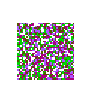
\includegraphics[scale=1.5]{LabelsGamma0point5K5}
  \caption*{$\gamma_0=0.5$}
 \end{minipage} \hfill
 \begin{minipage}[htb]{0.24\linewidth}
  \centering
  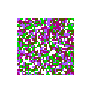
\includegraphics[scale=1.5]{LabelsGamma0point7K5}
  \caption*{$\gamma_0=0.7$}
 \end{minipage} \hfill
 \begin{minipage}[htb]{0.24\linewidth}
  \centering
  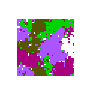
\includegraphics[scale=1.5]{LabelsGamma0point8K5}
  \caption*{$\gamma_0=0.8$}
 \end{minipage} \hfill
 \begin{minipage}[htb]{0.24\linewidth}
  \centering
  
\includegraphics[scale=1.5]{LabelsGamma1point6K5}
  \caption*{$\gamma_0=1.6$}
 \end{minipage} 
 \caption{Potts field for different values of $\gamma_0$}
 \label{fig:Potts field for different values of gamma_0}
\end{figure}
\end{enumerate}
\end{block}
\end{frame}

\begin{frame}{Prior Models}
\begin{block}{Hierarchical Model}
\bfig[htb]
\bcc
\begin{picture}(60,150)
  \put(-15,115){\framebox(20,15){$K$}}
  \put(-5,115){\line(0,-1){45}}
  \put(-5, 70){\vector(-1, 0){25}}

  \put(-50,115){\framebox(20,15){$\gamma_0$}}
  \put(-40,115){\vector(0,-1){35}}
  
  \put(-85,115){\framebox(20,15){$\alphab$}}
  \put(-75,115){\line(0,-1){45}}
  \put(-75, 70){\vector(1, 0){25}}

  \put(-40,70){\makebox(0,0){$\rzb$}}
  \put(-40,70){\circle{20}}
  \put(-40, 60){\line(0, -1){20}}
  \put(-40, 40){\vector(1, 0){60}}

  \put(12.5,115){\framebox(30,15){$m_0,v_0$}}
  \put(30,115){\vector(0,-1){35}}
  \put(30,70){\circle{20}}
  \put(30,70){\makebox(0,0){$\rmb$}}
  \put(30,60){\vector(0,-1){10}}
  
  \put(48,115){\framebox(30,15){$\alpha_0,\beta_0$}}
  \put(65,115){\vector(0,-1){35}}
  \put(65,70){\makebox(0,0){$\rvb$}}
  \put(65,70){\circle{20}}
  \put(65,60){\line(0,-1){20}}
  \put(65,40){\vector(-1,0){25}}
  
  \put(83.5,115){\framebox(34,15){$\alphaez,\betaez$}}
  \put(100.5,115){\vector(0,-1){35}}
  \put(100.5,70){\makebox(0,0){$\red{\vb_{\epsilon}}$}}
  \put(100.5,70){\circle{20}}

  \put(30,40){\makebox(0,0){$\rfb$}}
  \put(30,40){\circle{20}}

  \put(100.5,60){\line(0,-1){60}}
  \put(100.5,0){\vector(-1,0){60.5}}
  
  \put(30,30){\vector(0,-1){20}}
  \put(25,20){\makebox(0,0){$\Hb$}}
  \put(30,0){\circle{20}}
  \put(30,0){\makebox(0,0){$\bgb$}}
   
 \end{picture}
\ecc
\efig
\end{block}
\end{frame}

\begin{frame}{Joint Maximization a Posteriori (JMAP)}
\begin{block}{Use of Bayes rule}
\begin{enumerate}
\item Estimate the unknowns $\fb, \zb, \vb_{\epsilon}, \mb$ and $\vb$ by maximizing their joint posterior probability
\beq
(\hat{\rfb},\hat{\rzb},\hat{\rvb}_{\red{\epsilon}},\hat{\rmb},\hat{\rvb})=
\argmax{(\rfb,\rzb,\red{\vb_{\epsilon}},\rmb,\rvb)}{p(\rfb,\rzb,\red{\vb_{\epsilon}},\rmb,\rvb|\bgb;\Mc)}
\eeq
\item An alternate optimization scheme is found by applying Bayes rule
\beq
\barr{ll}
p(\rfb,\rzb,\red{\vb_{\epsilon}},\rmb,\rvb|\bgb;\Mc)&\propto 
p(\bgb|\rfb,\red{\vb_{\epsilon}})\, p(\rfb|\rzb,\rmb,\rvb) \, \\ 
&p(\red{\vb_{\epsilon}}|\alphaez,\betaez)\, 
p(\rzb|\alphab; \gamma_0) \, \\
&p(\rmb|m_{0}, v_{0})\, p(\rvb|\alpha_0, \beta_0), 
\earr
\eeq
\end{enumerate}
\end{block}
\end{frame}

\begin{frame}{Joint Maximization a Posteriori (JMAP)}
% The iterative update of each unknown yields a criterion for estimating the volume. Each hyperparameters of the criterion are optimal for the controlled volume thanks to the joint estimation
\begin{block}{Alternate optimization}
\bfig[htb]
\bcc
\begin{picture}(200,150)
  \put(40,140){\framebox(180,20){1 : update volume \red{\fb} (minimize $J(\rfb)$)}}
  \put(130,140){\line(0,-1){10}}
  \put(130,130){\line(-1,0){85}}
  \put(45,130){\vector(0,-1){10}}
  \put(-20,100){\framebox(130,20){2 : update uncertainties $\red{\vb_{\epsilon}}$}}
  \put(45,100){\vector(0,-1){100}}
  \put(130,130){\line(1,0){65}}
  \put(195,130){\vector(0,-1){10}}
  \put(150,100){\framebox(90,20){3 : update labels $\red{\zb}$}}
  \put(195,100){\vector(0,-1){20}}
  \put(145,60){\framebox(100,20){4 : update means $\red{\mb}$}}
  \put(195,60){\vector(0,-1){20}}
  \put(140,20){\framebox(110,20){5 : update variances $\red{\vb}$}}
  \put(195,20){\vector(0,-1){20}}
  
  
  \put(-10,-20){\makebox(0,0){$J(\rfb)=$}}
  \put(55,-20){\makebox(0,0){$\|\bgb-\Hb\rfb\|_{\red{\Vb_{\epsilon}}}^{2}$}}
  \put(120,-20){\makebox(0,0){$+$}}
  \put(205,-20){\makebox(0,0){$\|\rfb-\rmb_{\rzb}\|_{\red{\Vb_{\zb}}}^{2}$}}
  \put(-30,-20){\line(-1,0){20}}
  \put(-50,-20){\line(0,1){170}}
  \put(-50,150){\vector(1,0){90}}
   
\end{picture}
\ecc
\efig
\end{block}
\end{frame}

\begin{frame}{Results on real 3D data}
\begin{block}{Data}
\begin{enumerate}
\item Test on patented real IQI (Image Quality Indicator) \cite{gay2016fantomeiqi} with $512 \times 512 \times 256$ voxels
\item $300$ projections are used, with $512 \times 256$ pixels
\item $K=4$ materials
%% volume original
\begin{figure}
\begin{minipage}[htb]{0.46\linewidth}
\centering
\includegraphics[scale=0.25]{volume_FDK2400projBas.png}
\end{minipage} \hfill
\begin{minipage}[htb]{0.46\linewidth}
\centering
\includegraphics[scale=0.25]{volume_FDK2400projHaut.png}
\end{minipage}
\caption*{Real IQI phantom (bottom and top) (retrieved from avec 2400 projections)}
\label{fig:Real IQI data}
\end{figure}
\end{enumerate}
\end{block}
\end{frame}

\begin{frame}{Results on real 3D data}
\begin{block}{Strategies to fix the parameters}
\begin{enumerate}
\item Prior on the volume : use of a first estimate $\rfb^{(0)}$ (FDK) :
\beq
m_{0}=\frac{1}{2}\left(\max_{j}{\red{f_{j}}^{(0)}}+\min_{j}{\red{f_{j}}^{(0)}}\right)
\eeq
Parameters $v_0, \alpha_0$ and $\beta_0$ fixed so that the support of the distributions $\Nc(m_0, v_0)$ and $\Ic\Gc(\alpha_0, \beta_0)$ is sufficiently large for the considered volume
\item Prior on the projection : use a prior on the SNR : SNR=20 dB. Fix $\alphaez$ and
\beq
\betaez=\frac{\alphaez-1}{M}\times\|\bgb\|^{2}\times \frac{10^{-\frac{SNR}{10}}}{1+10^{-\frac{SNR}{10}}}.
\label{eq:betaez}
\eeq
\end{enumerate}
\end{block}
\end{frame}

\begin{frame}{Results on real 3D data}
\begin{block}{Strategies to fix the parameters}
\begin{enumerate}
\item Potts coefficient is fixed empirically in order to have compact classes
\item A possible improvement would be to use an automatic and fast algorithm to fix this parameter at initialization
\begin{table}[htb]
\begin{center}
\begin{tabular}{|*{7}{c|}}
\hline
\textbf{Parameters} & $\alphaez$ & $K$ & $\gamma_{0}$ & $v_0$ & $\alpha_0$ & $\beta_0$ \\
\hline
Fixed values & 2.1 & 4 & 3 & 1 & 5 & 0.01 \\
\hline
\end{tabular}
\end{center}
\caption{Reconstruction parameters for 3D IQI data}
\label{tab:Reconstruction parameters}
\end{table}
\end{enumerate}
\end{block}
\end{frame}

\begin{frame}{Results on real 3D data}
\begin{block}{Reconstruction quality indicators}
\begin{enumerate}
\item The jointly retrieved reconstruction and segmentation can be used to quantify the quality of the reconstruction
\item A reconstruction is considered to be good if it has compact, quite homogeneous and distinguishable classes
\item We define reconstruction quality indicators which do not need reference.
\end{enumerate}
\end{block}
\end{frame}

\begin{frame}{Results on real 3D data}
\begin{block}{Compactness indicator for the reconstruction}
\begin{enumerate}
\item Quantify how compact the classes are :
\beq
C_{omp}=\frac{1}{K}\sum_{k=1}^{K}\frac{1}{\red{N_k}}\sum_{j \in \red{\Rc_k}}\frac{1}{N_{\Vc}}\sum_{i \in \Vc(j)} \delta(k-\red{z_i})
\label{eq:compacity at voxel's scale}
\eeq
where $N_{\Vc}$ is the number of neighbours : $N_{\Vc}=6$.
\end{enumerate}
\end{block}
\end{frame}

\begin{frame}{Results on real 3D data}
\begin{block}{Homogeneity indicator for the reconstruction}
\begin{enumerate}
\item Quantify how homogeneous the classes are
\beq
h_{omo}=\frac{1}{K}\sum_{k=1}^{K}\frac{1}{\red{N_k}}\sum_{j \in \red{\Rc_k}}(\hat{h}_{omo})_{j}
\eeq
with, if $\red{z_j}=k$ :
\beq
(\hat{h}_{omo})_{j}=
\frac{\sum_{i \in \Vc(j)}\exp\left(-(\red{f_j}-\red{f_i})^{2}\right)\delta(k-\red{z_i})}{\sum_{i \in \Vc(j)}\delta(k-\red{z_i})}
\eeq
if $\sum_{i \in \Vc(j)}\delta(k-\red{z_i}) \neq 0$. Otherwise, $(\hat{h}_{omo})_{j}=0$
\end{enumerate}
\end{block}
\end{frame}

\begin{frame}{Results on real 3D data}
\begin{block}{Distinguishability indicator for the reconstruction}
\begin{enumerate}
\item Quantify how distinguishable the classes are
\beq
d_{ist}=1-\frac{1}{K}\sum_{k=1}^{K}\frac{1}{\red{N_k}}\sum_{j \in \red{\Rc_k}}(\hat{d}_{ist})_{j}
\eeq
with, if $\red{z_j}=k$ :
\beq
(\hat{d}_{ist})_{j}=
\left\{
\barr{ll}
&\frac{\sum_{i \in \Vc(j)}\exp\left(-(\red{f_j}-\red{f_i})^{2}\right)(1-\delta(k-\red{z_i}))}{\sum_{i \in \Vc(j)}(1-\delta(k-\red{z_i}))} \mbox{~~if $j$ is on a~~} \\
&\mbox{~~\hspace*{43mm} contour~~} \\
&0 \mbox{~~otherwise~~}
\earr
\right.
\eeq
\end{enumerate}
\end{block}
\end{frame}

\begin{frame}{Results on real 3D data}
\begin{block}{Comparison with other methods}
\begin{enumerate}
\item Comparison with FDK and Total Variation Minimization (TV)
\item In order to apply our reconstruction quality indicators, FDK and TV reconstructions are post-segmented using a Gauss-Markov-Potts prior model (same model as before excepted that $\Hb$ is replaced by $\Ib_N$)
\end{enumerate}
\end{block}
\end{frame}

\begin{frame}{}
\begin{block}{Results on real 3D data : Reconstructions (bottom and top)}
\begin{figure}
%FDK
\begin{minipage}[htb]{0.30\linewidth}
\centering
\includegraphics[scale=0.19]{volume_FDKProj300Bas.png}
\end{minipage} \hfill
%TV
\begin{minipage}[htb]{0.30\linewidth}
\centering
\includegraphics[scale=0.19]{volumeIQI_TVProj300Bas.png}
\end{minipage} \hfill
%JMAP
\begin{minipage}[htb]{0.30\linewidth}
\centering
\includegraphics[scale=0.19]{volumeIQI_JMAPPottsIndGamma3K4Proj300Bas.png}
\end{minipage} \vfill
%FDK
\begin{minipage}[htb]{0.30\linewidth}
\centering
\includegraphics[scale=0.19]{volume_FDKProj300Haut.png}
\caption*{FDK}
\end{minipage} \hfill
%TV
\begin{minipage}[htb]{0.30\linewidth}
\centering
\includegraphics[scale=0.19]{volumeIQI_TVProj300Haut.png}
\caption*{TV}
\end{minipage} \hfill
%JMAP
\begin{minipage}[htb]{0.30\linewidth}
\centering
\includegraphics[scale=0.19]{volumeIQI_JMAPPottsIndGamma3K4Proj300Haut.png}
\caption*{JMAP}
\end{minipage}
\end{figure}
\end{block}
\end{frame}

\begin{frame}{}
\begin{block}{Results on real 3D data : Segmentations (bottom and top)}
\begin{figure}
%FDK
\begin{minipage}[htb]{0.30\linewidth}
\centering
\includegraphics[scale=0.19]{segmentation_FDKK4Proj300Bas.png}
\end{minipage} \hfill
%TV
\begin{minipage}[htb]{0.30\linewidth}
\centering
\includegraphics[scale=0.19]{segmentationIQI_TVGamma3K4Proj300Bas.png}
\end{minipage} \hfill
%JMAP
\begin{minipage}[htb]{0.30\linewidth}
\centering
\includegraphics[scale=0.19]{segmentationIQI_JMAPPottsIndGamma3K4Proj300Bas.png}
\end{minipage} \vfill
%FDK
\begin{minipage}[htb]{0.30\linewidth}
\centering
\includegraphics[scale=0.19]{segmentation_FDKK4Proj300Haut.png}
\caption*{FDK}
\end{minipage} \hfill
%TV
\begin{minipage}[htb]{0.30\linewidth}
\centering
\includegraphics[scale=0.19]{segmentationIQI_TVGamma3K4Proj300Haut.png}
\caption*{TV}
\end{minipage} \hfill
%JMAP
\begin{minipage}[htb]{0.30\linewidth}
\centering
\includegraphics[scale=0.19]{segmentationIQI_JMAPPottsIndGamma3K4Proj300Haut.png}
\caption*{JMAP}
\end{minipage}
\end{figure}
\end{block}
\end{frame}

\begin{frame}{Results on real 3D data}
\begin{block}{Comparison with other methods}
\begin{enumerate}
\item JMAP algorithm retrieves the reconstruction with the best contrast
\item We compute the reconstruction quality indicators
\begin{table}[htb]
\begin{center}
\begin{tabular}{|*{4}{c|}}
\hline
\textbf{Indicator} & $C_{omp}$ & $d_{ist}$ & $h_{omo}$  \\
\hline
FDK & 94.4 \% & 78.4 \% & 78.3 \% \\
\hline
TV & \textbf{94.5} \% & 77.5 \% & 77.5 \% \\
\hline
JMAP & 94.3 \% & \textbf{79.0} \% & \textbf{78.8} \% \\
\hline
\end{tabular}
\end{center}
\label{tab:Comparison of FDK and JMAP using reconstruction quality indicators}
\end{table} 
\item JMAP algorithm retrieves the reconstruction with the most distinguishable and homogeneous classes
\item More discriminating reconstruction quality indicators shall be studied
\end{enumerate}
\end{block}
\end{frame}

\begin{frame}{Results on real 3D data}
% We compare the profile of the holes : best contrast for JMAP
\begin{block}{Measure the resolution : profiles of the holes}
\begin{figure}
\begin{minipage}[htb]{0.46\linewidth}
\centering
\includegraphics[scale=0.30]{AnalyzeHolesVolIQI_FDKProj300.png}
\caption*{FDK}
\end{minipage} \hfill
\begin{minipage}[htb]{0.46\linewidth}
\centering
\includegraphics[scale=0.30]{AnalyzeHolesVolIQI_TVProj300.png}
\caption*{TV}
\end{minipage} \vfill
\begin{minipage}[htb]{0.46\linewidth}
\centering
\includegraphics[scale=0.27]{TraceProfileHoleHorizontal.png}
\end{minipage} \hfill
\begin{minipage}[htb]{0.46\linewidth}
\centering
\includegraphics[scale=0.30]{AnalyzeHolesVolIQI_JMAPGamma3K4Proj300.png}
\caption*{JMAP}
\end{minipage}
\label{fig:Profiles of holes for FDK (a) and JMAP (b) reconstructions}
\end{figure}
\end{block}
\end{frame}

\begin{frame}{Results on real 3D data}
\begin{block}{Measure the resolution : Peak height ratio}
\begin{minipage}[htb]{0.46\linewidth}
\begin{figure}
\centering
\includegraphics[scale=0.27]{PeakHeightRatio100pourcent.png}
\caption*{Diameter of the holes : 1.2 mm}
\end{figure}
\end{minipage} \hfill
\begin{minipage}[htb]{0.46\linewidth}
\centering
\includegraphics[scale=0.27]{TraceProfileHole.png}
\end{minipage} \vfill
\begin{minipage}[htb]{0.46\linewidth}
\begin{figure}
\centering
\includegraphics[scale=0.27]{PeakHeightRatio90pourcent.png}
\caption*{Diameter of the holes : 0.5 mm}
\end{figure}
\end{minipage} \hfill
\begin{minipage}[htb]{0.46\linewidth}
\begin{enumerate}
\item Plot the profile for each pair of holes, with different diameters
\item Compute the peak height ratio : $r_h=\frac{h_{up}}{h_{down}}$
\end{enumerate}
\end{minipage}
\end{block}
\end{frame}

\begin{frame}{Results on real 3D data}
\begin{block}{Comparison of the peak height ratio}
% best resolution for JMAP
\begin{minipage}[htb]{\linewidth}
\centering
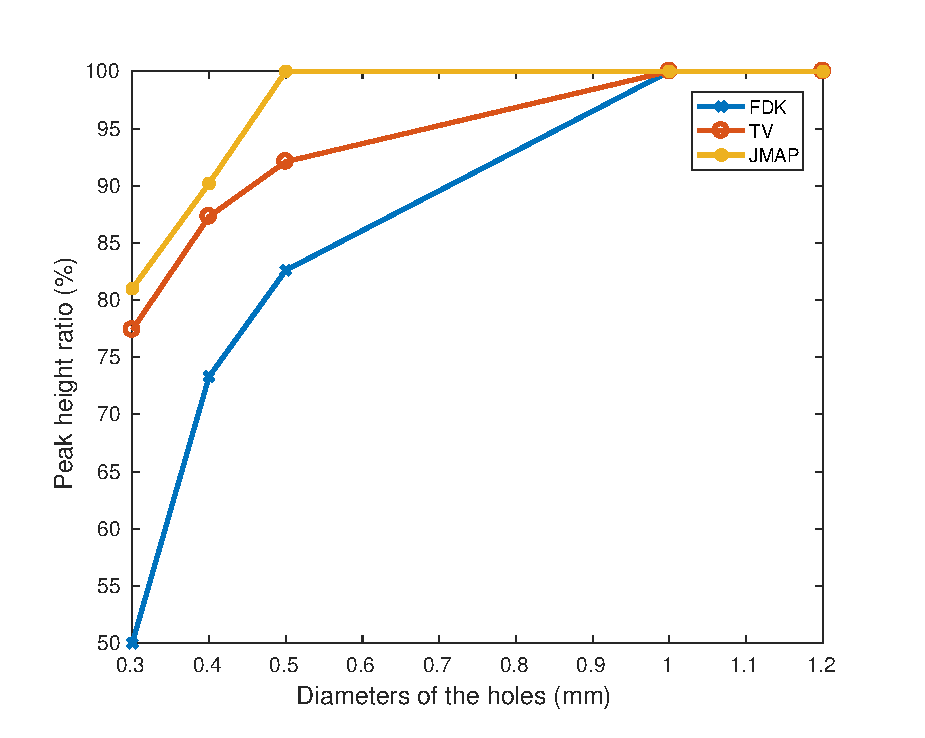
\includegraphics[scale=0.38]{PeakHeightRatio}
\end{minipage} \vfill
\begin{minipage}[htb]{\linewidth}
\begin{table}[htb]
\begin{center}
\begin{tabular}{|*{6}{c|}}
\hline
\textbf{Diameter (mm)} & $1.02$ & $1.0$ & $0.5$ & $0.4$ & $0.3$ \\
\hline
FDK & \textbf{100} \% & \textbf{100} \% & 82.6 \% & 73.3 \% & 50.0 \% \\
\hline
TV & \textbf{100} \% & \textbf{100} \% & 92.1 \% & 87.3 \% & 77.4 \% \\
\hline
JMAP & \textbf{100} \% & \textbf{100} \% & \textbf{100} \% & \textbf{90.2} \% & \textbf{81.0} \% \\
\hline
\end{tabular}
\end{center}
\caption{Comparison of $r_h$ for different pairs of holes}
\end{table} 
\end{minipage}
\end{block}
\end{frame}

\begin{frame}{Conclusion and prospects}
\begin{enumerate}
\item We proposed a highly-parallelizable joint reconstruction and segmentation algorithm which obtained good results for reconstructing industrial parts
\item The segmentation is used to provide an optimized regularization in order to estimate the volume 
\item The labels retrieved jointly with the reconstruction shall be useful for NDT
\item The retrieved reconstruction for 3D IQI data has been shown to have better contrast and resolution than FDK and TV reconstructions.
\item For the moment, the segmentation step is performed on CPU and takes about $75 \%$ of the total computation time. An implementation of this step on GPU would greatly speed up the algorithm 
\end{enumerate}
\end{frame}

\begin{frame}
\begin{center}
\Huge
\blue{Thanks for your attention !}
\end{center}
\end{frame}

\begin{frame}{Acknowledgements}
The authors are grateful to Lionel Gay and Nicolas Cochennec from Safran Composites for having provided the real IQI phantom used to test the method.
\end{frame}

\begin{frame}
\begin{center}
\Huge
\blue{Appendix}
\end{center}
\end{frame}

\begin{frame}{Joint Maximization a Posteriori (JMAP)}
% The estimation of the volume is done by optimizing a criterion which is built by using the estimates of the other unknowns and the segmentation from the previous iterations
\begin{block}{Estimation of the volume}
\begin{enumerate}
\item A criterion built by using the segmentation found during the previous iteration is optimized
\item Maximizing
\beq
p(\rfb|\rzb, \red{\vb_{\epsilon}}, \rmb, \rvb; \bgb, \Mc)
\propto p(\bgb|\rfb,\red{\vb_{\epsilon}})\, p(\rfb|\rzb,\rmb,\rvb)
\eeq
leads to minimize
\begin{align*}
J(\rfb)&=\|\bgb-\Hb\rfb\|_{\red{\Vb_{\epsilon}}}^{2}+\|\rfb-\rmb_{\rzb}\|_{\red{\Vb_{\zb}}}^{2} \\
&=\|\bgb-\Hb\rfb\|_{\red{\Vb_{\epsilon}}}^{2}+\sum_{j=1}^{N}\sum_{k=1}^{K}\frac{\left(\red{f_{j}}-\red{m_{k}}\right)^{2}}{\red{v_{k}}}\delta(\red{z_j}-k)
\end{align*}
\item Simple gradient descent with optimal step computing is performed
\end{enumerate}
\end{block}
\end{frame}

\begin{frame}{Joint Maximization a Posteriori (JMAP)}
% ICM gives good results for estimating the labels with minimum computational cost in a highly-parallelizable way
\begin{block}{Estimation of the labels}
\bfig[h]
\begin{minipage}[htb]{0.46\linewidth}
\centering
\includegraphics[scale=0.23]{BlancsNoirsAyasso}
\end{minipage} \hfill
\begin{minipage}[htb]{0.46\linewidth}
\bcc
\begin{picture}(60,70)

  \put(30,50){\makebox(0,0){maximize $E(\rzb_{\red{N}}|\rfb, \rzb_{\red{B}}, \rmb, \rvb;\Mc)$}}
  
  \put(30,40){\vector(0,-1){10}}
  \put(30,20){\makebox(0,0){maximize $E(\rzb_{\red{B}}|\rfb, \rzb_{\red{N}}, \rmb, \rvb; \Mc)$}}
  \put(30, 10){\line(0, -1){10}}
  \put(30, 0){\line(-1, 0){90}}
  \put(-60, 0){\line(0, 1){70}}
  \put(-60, 70){\line(1, 0){90}}
  \put(30, 70){\vector(0, -1){10}}
   
 \end{picture}
\ecc
\end{minipage}
\efig\textit{Iterated Conditional Modes} (ICM) to maximize Potts energy
\begin{align*}
E(\rzb|\rfb,\rmb,\rvb;\Mc)&=\sum_{j=1}^{N}\left[\sum_{k=1}^{K}\left(
\alpha_k-\frac{\left(\red{f_{j}}-\red{m_{k}}\right)^{2}}{2 \red{v_{k}}}-\frac{1}{2}\ln{(\red{v_k})}\right)\delta(\red{z_j}-k)\right. \\
&\left.+\gamma_0\sum_{i\in\Vc(j)}\delta(\red{z_j}-\red{z_i})\right]
\end{align*}
\end{block}
\end{frame}

\begin{frame}{Joint Maximization a Posteriori (JMAP)}
% The estimations of the other unknowns are given by analytical formulas thanks to the use of conjugate priors
\begin{block}{Estimation of the other unknowns}
\begin{enumerate}
\item Conjugate priors give analytical formulas
\beq
\hat{\red{v}}_{\red{\epsilon_{i}}}=\frac{\betaez+\frac{1}{2}\left(\blue{g_{i}}-\lbrack\Hb\rfb\rbrack_{i}\right)^{2}}{\alphaez+\frac{3}{2}}, \forall i \in \left\{ 1, \dots, M \right\},
\eeq
\beq
\hat{\red{m}}_{\red{k}}=\frac{m_0+\frac{v_0}{\red{v_{k}}}\sum_{j \in \red{\Rc_{k}}}\red{f_{j}}}{1+\frac{\red{N_{k}}v_0}{\red{v_{k}}}}, \forall k \in \left\{ 1, \dots, K \right\}
\eeq
and
\beq
\hat{\red{v}}_{\red{k}}=\frac{\beta_0+\frac{1}{2}\sum_{j \in \red{\Rc_{k}}}\left(\red{f_{j}}-\red{m_{k}}\right)^{2}}{\alpha_0+\frac{\red{N_{k}}}{2}+1}, \forall k \in \left\{ 1, \dots, K \right\}
\eeq
where $\red{N_k}$ is the number of voxels in class $k$ $\red{\Rc_k}$.
\end{enumerate}
\end{block}
\end{frame}

\begin{frame}{Strategies to fix the parameters}
\begin{block}{Fixing $\betaez$}
\begin{enumerate}
\item $p(\red{v_{\epsilon_{i}}}|\alphaez,\betaez)=\Ic\Gc(\red{v_{\epsilon_{i}}}|\alphaez,\betaez), \forall i$
\item $SNR=10\log\left(\frac{\|\red{\gb_{0}}\|^{2}}{\|\red{\epsilonb}\|^{2}}\right)$
\item Assumption : the noise $\epsilonb$ and the unnoisy projections $\gb_{0}$ are orthogonal :
\beq
\|\bgb\|^{2}=\|\red{\gb_{0}}\|^{2}+\|\red{\epsilonb}\|^{2}
\label{eq:Noise and unnoisy data orthogonal}
\eeq
\item So : 
\beq
SNR=10\log\left(\frac{\|\bgb\|^{2}}{\|\red{\epsilonb}\|^{2}}-1\right)
\eeq
\end{enumerate}
\end{block}
\end{frame}

\begin{frame}{Strategies to fix the parameters}
\begin{block}{Fixing $\betaez$}
\begin{enumerate}
\item Approximate $\|\epsilonb\|^{2}$ by its expectation :
\begin{align*}
\|\red{\epsilonb}\|^{2} &\approx \mathbb{E}\left(\red{\epsilonb}^{T}\red{\epsilonb}\right)
=\Tr{\mathbb{E}(\red{\epsilonb}\red{\epsilonb}^{T})}=\Tr{\mathbb{E}\left(\mathbb{E}\left(\red{\epsilonb}\red{\epsilonb}^{T}|\red{\Vb_{\epsilon}}\right)\right)} \\
&=\Tr{\mathbb{E}\left(\red{\Vb_{\epsilon}}\right)}=\mathbb{E}\left(\Tr{\red{\Vb_{\epsilon}}}\right)=\mathbb{E}\left(\sum_{i=1}^{M} \red{v_{\epsilon_{i}}}\right) \\
&=\sum_{i=1}^{M}\mathbb{E}\left(\red{v_{\epsilon_{i}}}\right)=M \times \frac{\betaez}{\left(\alphaez-1\right)}
\end{align*}
\item So :
\beq
\betaez=\frac{\alphaez-1}{M}\times\|\bgb\|^{2}\times \frac{10^{-\frac{SNR}{10}}}{1+10^{-\frac{SNR}{10}}}.
\label{eq:betaez appendix}
\eeq
\end{enumerate}
\end{block}
\end{frame}

\begin{frame}{Profiles of the holes for each pair of holes}
\begin{block}{Diameter : 1.2 mm}
\begin{figure}
\begin{minipage}[htb]{0.46\linewidth}
\centering
\includegraphics[scale=0.27]{ProfilsTrousIQICalculResolution/FDK/300proj/ProfilTrousTaille1.png}
\caption*{FDK}
\end{minipage} \hfill
\begin{minipage}[htb]{0.46\linewidth}
\centering
\includegraphics[scale=0.27]{ProfilsTrousIQICalculResolution/TV/300proj/ProfilTrousTaille1.png}
\caption*{TV}
\end{minipage} \vfill
\begin{minipage}[htb]{0.46\linewidth}
\centering
\includegraphics[scale=0.27]{ProfilsTrousIQICalculResolution/JMAPMGINonSplitGamma3K4/300proj/ProfilTrousTaille1.png}
\caption*{JMAP}
\end{minipage}
\end{figure}
\end{block}
\end{frame}

\begin{frame}{Profiles of the holes for each pair of holes}
\begin{block}{Diameter : 1.0 mm}
\begin{figure}
\begin{minipage}[htb]{0.46\linewidth}
\centering
\includegraphics[scale=0.27]{ProfilsTrousIQICalculResolution/FDK/300proj/ProfilTrousTaille2.png}
\caption*{FDK}
\end{minipage} \hfill
\begin{minipage}[htb]{0.46\linewidth}
\centering
\includegraphics[scale=0.27]{ProfilsTrousIQICalculResolution/TV/300proj/ProfilTrousTaille2.png}
\caption*{TV}
\end{minipage} \vfill
\begin{minipage}[htb]{0.46\linewidth}
\centering
\includegraphics[scale=0.27]{ProfilsTrousIQICalculResolution/JMAPMGINonSplitGamma3K4/300proj/ProfilTrousTaille2.png}
\caption*{JMAP}
\end{minipage}
\end{figure}
\end{block}
\end{frame}

\begin{frame}{Profiles of the holes for each pair of holes}
\begin{block}{Diameter : 0.5 mm}
\begin{figure}
\begin{minipage}[htb]{0.46\linewidth}
\centering
\includegraphics[scale=0.27]{ProfilsTrousIQICalculResolution/FDK/300proj/ProfilTrousTaille3.png}
\caption*{FDK}
\end{minipage} \hfill
\begin{minipage}[htb]{0.46\linewidth}
\centering
\includegraphics[scale=0.27]{ProfilsTrousIQICalculResolution/TV/300proj/ProfilTrousTaille3.png}
\caption*{TV}
\end{minipage} \vfill
\begin{minipage}[htb]{0.46\linewidth}
\centering
\includegraphics[scale=0.27]{ProfilsTrousIQICalculResolution/JMAPMGINonSplitGamma3K4/300proj/ProfilTrousTaille3.png}
\caption*{JMAP}
\end{minipage}
\end{figure}
\end{block}
\end{frame}

\begin{frame}{Profiles of the holes for each pair of holes}
\begin{block}{Diameter : 0.4 mm}
\begin{figure}
\begin{minipage}[htb]{0.46\linewidth}
\centering
\includegraphics[scale=0.27]{ProfilsTrousIQICalculResolution/FDK/300proj/ProfilTrousTaille4.png}
\caption*{FDK}
\end{minipage} \hfill
\begin{minipage}[htb]{0.46\linewidth}
\centering
\includegraphics[scale=0.27]{ProfilsTrousIQICalculResolution/TV/300proj/ProfilTrousTaille4.png}
\caption*{TV}
\end{minipage} \vfill
\begin{minipage}[htb]{0.46\linewidth}
\centering
\includegraphics[scale=0.27]{ProfilsTrousIQICalculResolution/JMAPMGINonSplitGamma3K4/300proj/ProfilTrousTaille4.png}
\caption*{JMAP}
\end{minipage}
\end{figure}
\end{block}
\end{frame}

\begin{frame}{Profiles of the holes for each pair of holes}
\begin{block}{Diameter : 0.3 mm}
\begin{figure}
\begin{minipage}[htb]{0.46\linewidth}
\centering
\includegraphics[scale=0.27]{ProfilsTrousIQICalculResolution/FDK/300proj/ProfilTrousTaille5.png}
\caption*{FDK}
\end{minipage} \hfill
\begin{minipage}[htb]{0.46\linewidth}
\centering
\includegraphics[scale=0.27]{ProfilsTrousIQICalculResolution/TV/300proj/ProfilTrousTaille5.png}
\caption*{TV}
\end{minipage} \vfill
\begin{minipage}[htb]{0.46\linewidth}
\centering
\includegraphics[scale=0.27]{ProfilsTrousIQICalculResolution/JMAPMGINonSplitGamma3K4/300proj/ProfilTrousTaille5.png}
\caption*{JMAP}
\end{minipage}
\end{figure}
\end{block}
\end{frame}

\begin{frame}{References}
\bibliographystyle{ieeetr}
\bibliography{ChapdelaineBibliographie}
\end{frame}

\end{document}